%	file:		thesis.tex
%	author:	alex c. williams
%	updated:	6 May 2015

%	description:
%	this file provides a template for the mtsu computer science thesis.
%
%	NOTES
%	1. Chapter Headings should be bold in the "text" portion of the document.
%	- To fix:
%		1. add /textbf to each /chapter{} line
%		2. compile
%		3. remove \textnormal from the \thesection renew command.
%		4. compile
%
%	2. To change "Professor One" and etc., you need to modify the names in the complementary "committee_header.tex" file.

\documentclass[12pt, oneside]{book}

% Include these packages:
\usepackage[top=3.17cm, bottom=2.54cm, left=3.81cm, right=2.54cm]{geometry}	 % for margin requirements.
\usepackage{mathptmx}% http://ctan.org/pkg/mathptmx
\usepackage{amsmath}
\usepackage{setspace} % for double-spacing.
\usepackage{xifthen}%
\doublespacing
\usepackage{lipsum}
\usepackage{tocloft}
\usepackage{color}
\usepackage{array}
\usepackage{stfloats}
\usepackage[pdftex]{graphicx}
\usepackage{subcaption}
\usepackage[export]{adjustbox}
\usepackage{multirow}
\usepackage{url}
\usepackage{changepage}
\usepackage{floatrow}
\usepackage{titlesec}
%\usepackage{fancyhdr}
\usepackage{chngcntr}
\usepackage{fancyhdr}
\usepackage{verbatim} % for multi-line comments
% \begin{comment}  \end{comment}

% -- Define code snippet configuration
\usepackage{listings}
\usepackage{color}

\definecolor{dkgreen}{rgb}{0,0.6,0}
\definecolor{gray}{rgb}{0.5,0.5,0.5}
\definecolor{mauve}{rgb}{0.58,0,0.82}

\lstset{frame=tb,
  language=Python,
  aboveskip=3mm,
  belowskip=3mm,
  showstringspaces=false,
  columns=flexible,
  basicstyle={\small\ttfamily},
  numbers=none,
  numberstyle=\tiny\color{gray},
  keywordstyle=\color{blue},
  commentstyle=\color{dkgreen},
  stringstyle=\color{mauve},
  breaklines=true,
  breakatwhitespace=true,
  tabsize=3
}

% -- Base Page Styling 
\floatsetup[table]{capposition=top}
\counterwithout{figure}{chapter}
\counterwithout{table}{chapter}
\setlength\textfloatsep{18mm}
\fancyhf{}
\fancyhead[R]{\thepage}

% -- Base Styling for Section/Subsection/Subsubsection --
\titlespacing{\section}{0pt}{\parskip}{-\parskip}
\titlespacing{\subsection}{0pt}{\parskip}{-\parskip}
\titlespacing{\subsubsection}{0pt}{\parskip}{-\parskip}

% Styling for Section Headers
\titleformat{\section}
{\normalfont\bfseries\filcenter}
{\textnormal\thesection}
{0cm}
{}

% Styling for Subsection Headers
\titleformat{\subsection}
{\normalfont\filcenter}
{\textnormal\thesubsection}
{0cm}
{}

% -- Stylize Subfigure Headings--
\newlength\Origarrayrulewidth
\renewcommand{\thesubfigure}{\Alph{subfigure}}
\newcommand{\Cline}[1]{%
 \noalign{\global\setlength\Origarrayrulewidth{\arrayrulewidth}}%
 \noalign{\global\setlength\arrayrulewidth{2pt}}\cline{#1}%
 \noalign{\global\setlength\arrayrulewidth{\Origarrayrulewidth}}%
}
\newcommand\Thickvrule[1]{%
  \multicolumn{1}{!{\vrule width 2pt}c!{\vrule width 2pt}}{#1}%
}

% -- Stylize the Table of Contents --
\renewcommand{\cfttoctitlefont}{\hfill\normalsize}
\renewcommand*\thesubsection{}
\renewcommand*\thesection{\textnormal}
\renewcommand*\thechapter{\Roman{chapter}.}
\renewcommand*\thepart{}
\renewcommand\cftchapfont{\mdseries}
\renewcommand{\cftchapleader}{\cftdotfill{\cftdotsep}}
\renewcommand\cftchappagefont{\normalfont}
\renewcommand\cftpartpagefont{\normalfont}
\renewcommand\contentsname{\hfill{\textbf{TABLE OF CONTENTS}}\hfill}
\renewcommand{\cftaftertoctitle}{\hfill}
\renewcommand{\cftbeforepartskip}{1.00em}

% -- Stylize Chapter Headings --
\makeatletter
\let\orig@chapter\@chapter
\def\@chapter[#1]#2{\ifnum \c@secnumdepth >\m@ne
                       \if@mainmatter
                         \refstepcounter{chapter}%
                         \typeout{\@chapapp\space\thechapter.}%
                         \addcontentsline{toc}{chapter}%
                                   {\textnormal{CHAPTER}~\protect\numberline{\thechapter}#1}%
                       \else
                         \addcontentsline{toc}{chapter}{#1}%
                       \fi
                    \else
                      \addcontentsline{toc}{chapter}{#1}%
                    \fi
                    \chaptermark{#1}%
                    \addtocontents{lof}{\protect\addvspace{10\p@}}%
                    \addtocontents{lot}{\protect\addvspace{10\p@}}%
                    \if@twocolumn
                      \@topnewpage[\@makechapterhead{#2}]%
                    \else
                      \@makechapterhead{#2}%
                      \@afterheading
                    \fi}
\makeatother

% Patch for List of Figures extra spacing?? -mcm
\usepackage{etoolbox}% http://ctan.org/pkg/etoolbox
\makeatletter
% \patchcmd{<cmd>}{<search>}{<replace>}{<succes>}{<failure>}
\patchcmd{\@chapter}{\addtocontents{lof}{\protect\addvspace{10\p@}}}{}{}{}% LoF
\patchcmd{\@chapter}{\addtocontents{lot}{\protect\addvspace{10\p@}}}{}{}{}% LoT
\makeatother


% Stylize List of Figures
\renewcommand*\listfigurename{LIST OF FIGURES}
\renewcommand{\cftloftitlefont}{\hfill\normalsize}
\renewcommand{\cftafterloftitle}{\hfill}
\setlength{\cftbeforeloftitleskip}{-3em}
\setlength{\cftafterloftitleskip}{-0.05em}
\renewcommand{\cftfigfont}{Figure }


\usepackage{titlesec}
\usepackage[tracking=true]{microtype}
\titleformat{\chapter}[display]
  {\vspace{-2.54cm}\normalsize}
  {\filcenter\textbf{\MakeUppercase{\chaptertitlename} \thechapter}}
  {\parskip}
  {\filcenter\thispagestyle{myheadings}}

\titlespacing{\chapter}{0pt}{50pt}{\parskip}

\fancyhead[L]{}

% Stylize List of Tables
\renewcommand*\listtablename{LIST OF TABLES}
\renewcommand{\cftlottitlefont}{\hfill\normalsize}
\renewcommand{\cftafterlottitle}{\hfill}
\setlength{\cftbeforelottitleskip}{-3em}
\setlength{\cftafterlottitleskip}{-0.05em}
\renewcommand{\cfttabfont}{Table }
\renewcommand{\cftfigaftersnum}{ -- }
\renewcommand{\cfttabaftersnum}{ -- }

\renewcommand{\thefigure}{\arabic{figure}}
\renewcommand{\thetable}{\arabic{table}}
\renewcommand{\theequation}{}

% Stylize List of Symbols / Abbreviations -mcm
%\renewcommand*\listsymbolname{LIST OF SYMBOLS AND ABBREVIATIONS}
%\renewcommand{\cftlottitlefont}{\hfill\normalsize}
%\renewcommand{\cftafterlottitle}{\hfill}
%\setlength{\cftbeforelottitleskip}{-3em}
%\setlength{\cftafterlottitleskip}{-0.05em}





% -- Stylize Equations --
\makeatletter
\def\@eqnnum{{\normalfont \normalcolor \theequation}}
\makeatother

% -- Stylize Bibliography Title --
\renewcommand{\bibname}{\textbf{BIBLIOGRAPHY}}

% Include the dependency
% command for 
\newenvironment{nscenter}
 {\parskip=0pt\par\nopagebreak\centering}
 {\par\noindent\ignorespacesafterend}

% Change margins on-command.
\def\changemargin#1{\list{}{\leftmargin#1}\item[]}
\let\endchangemargin=\endlist 

% Macro:	addTitleAndAuthor
% Parameters:
%	- 1: Title Name
%	- 2: Your Name
\newcommand{\addTitleAndAuthor}[2]{
\begin{nscenter} 
\mbox{ }\\
  % Process Title..
#1% if #1 is not empty
\\[\baselineskip]

By\\[0\baselineskip]

#2
\\[2\baselineskip]% if #1 is not empty

\end{nscenter}
}

\newcommand{\addCommitteeMember}[2][Computer Science]{
	\ifthenelse{\isempty{#1}}
	{\\[0\baselineskip] \underline{\hspace{11.54cm}} \\[0\baselineskip] Dr. professor's name (Computer Science or other department)\\[0\baselineskip]}
	{\\[0\baselineskip] \underline{\hspace{11.54cm}} \\[0\baselineskip] Dr. {#2} (#1) \\[0\baselineskip]}
}


\newcommand{\addSupervisor}[2][Computer Science]{
	\ifthenelse{\isempty{#1}}
	{\\[0\baselineskip] \underline{\hspace{11.54cm}} \\[0\baselineskip] Supervisor Dr. professor's name (Computer Science) \\[0\baselineskip]}
	{\\[0\baselineskip] \underline{\hspace{11.54cm}} \\[0\baselineskip] Supervisor Dr. {#2} (#1) \\[0\baselineskip]}
}

\newcommand{\addChair}[1][Chair's Name]{
	\noindent\underline{\hspace{11.54cm}} \newline Dr. #1, Chairperson Computer Science Department \\
}

\newcommand{\addDean}[1][Dean's Name]{
	\noindent\underline{\hspace{11.54cm}} \newline Dr. #1, Interim Dean of the College of Graduate Studies \\
}

% Macro:	addCommittee
% Parameters:
%	- 1. Committee Member 1 (Supervisor)
%	- 2. Committee Member 1's Department
%	- 3. Committee Member 2
%	- 4. Committee Member 2's Department
%	- 5. Committee Member 3
%	- 6. Committee Member 3's Department
%	- 7. Computer Science Chairperson
%	- 8. Dean of Graduate Studies
\newcommand{\addCommittee}[8]{
	\noindent APPROVED: 
	\begin{changemargin}{2.54cm}
		Graduate Committee\vspace{1mm} \newline
		% set committee members
		\addSupervisor[#2]{#1}
		\addCommitteeMember[#4]{#3}
		\addCommitteeMember[#6]{#5}
	\end{changemargin}

	\addChair[#7]
	
	\addDean[#8]

}

\newcommand{\addDegreeNotes}[1]{
\vspace{8ex}
\centerline{A thesis submitted in partial fulfillment}
\centerline{of the requirements for the degree of}

\vspace{8ex}

\centerline{MASTER OF SCIENCE}
\centerline{in}
\centerline{Computer Science}

\vspace{8ex}

\centerline{Middle Tennessee State University}
\vspace{1ex}

\centerline{#1}

\vspace{8ex}

\centerline{Thesis Committee:}

\centerline{Dr. Joshua L. Phillips}

\centerline{Dr. Suk Seo}

\centerline{Dr. Lisa Green}

}

%\usepackage{fancyheadings}
\usepackage{fancyhdr}

% Document Formation
\begin{document}

% - - - Title Page - - -  REMOVE FOR FINAL SUBMISSION
% Add Title / Author
%\thispagestyle{empty}

%%%\addTitleAndAuthor	{\textbf{PRESERVING RELATIVE DIMENSION RANKINGS IN THE PRESENCE OF NOISE USING THE BOX-COUNTING ALGORITHM}} % Title
%%%				{Michael C. Murphy} % Author

% Add Committee
%%%\addCommittee{Joshua L. Phillips}{Computer Science}
%%%			{Suk Seo}{Computer Science}
%%%			{Lisa Green}{Mathematics}
%%%			{Chrisila Pettey}
%%%			{Jackie Eller}



%\newpage
% - - - Title Page (with MS/Graduation Date)
% Add Title / Author
\pagenumbering{roman}
\thispagestyle{empty}
\pagestyle{fancy}
\lhead{} \chead{} \rhead{}
\lfoot{} \cfoot{\thepage} \rfoot{}
\renewcommand{\headrulewidth}{0pt}
\renewcommand{\footrulewidth}{0pt}
\vspace{2ex}
\addTitleAndAuthor	{\textbf{Preserving Relative Dimension Rankings in the Presence of Noise Using the Box-Counting Algorithm}} % Title
				{Michael C. Murphy} % Author

% Specify Graduate Month
\addDegreeNotes{August 2016}

\newpage
% - - - Acknowledgments Page - - -
\centerline{\textbf{ACKNOWLEDGEMENTS}}

I would like to thank Dr. Phillips for his excellent guidance, suggestions, and encouragement throughout this entire project.  Dr. Phillips showed me that not only could I succeed at research, but enjoy the process along the way.

I would like to thank Dr. Patrick Murphy, my father, for introducing me to the fascinating topics of fractals and fractal dimension, and for his constant willingness to brainstorm new areas of exploration.  

I would like to thank fellow graduate Robert Myers for being a sounding board over the past six months and for his constructive feedback while writing and organizing this paper.  

Most of all, I'd like to thank my wife, Whitney Murphy, for being the most supportive partner one could ever hope for.  None of this would have been possible without her love and support, and this thesis is dedicated to her.


% =====================================================================
% 
%      A B S T R A C T
%
% =====================================================================
\newpage
\centerline{\textbf{ABSTRACT}}

Fractal dimension is a number that describes the degree of self-similarity, or "complexity", of a particular geometry.  In digital image processing, fractal dimension is often used to provide quantitative comparisons between digital images.  The Box-Counting Algorithm is one of the more widely used methods for estimating fractal dimension, although it has been shown to be highly sensitive to digital filtering and noise.  This research investigates the variability in fractal dimension estimates obtained from the Box-Counting Algorithm as noise is applied to an image.  In the case of increasing uniform noise, three distinct relationships emerge between dimensional estimates and their variability.  It is then shown how these relationships may be leveraged to improve relative rankings among dimensional estimates when using the Box-Counting Algorithm.  

%(122/150)

%\newpage
%\centerline{\textbf{PREFACE}}
%If you require a preface, type it here.

% - - - Table of Contents - - -
\newpage
\begingroup
\renewcommand{\vspace}[2]{}% Gobble 2 arguments after \vspace
\tableofcontents
\endgroup

\cleardoublepage
\clearpage

% - - - List of Tables - - -
\renewcommand\listtablename{\textnormal{LIST OF TABLES}}
\addcontentsline{toc}{chapter}{\listtablename}
\listoftables
\thispagestyle{plain}
\clearpage

% - - - List of Figures - - -
\renewcommand\listfigurename{\textnormal{LIST OF FIGURES}}
\addcontentsline{toc}{chapter}{\listfigurename}
\listoffigures
\clearpage

% - - - List of Symbols and Abbreviations -mcm
%\renewcommand\listsymbolname{\textnormal{LIST OF SYMBOLS AND ABBREVIATIONS}}
%\addcontentsline{toc}{chapter}{\listsymbolname}
%BCA - Box-Count Algorithm
%\clearpage


\newpage
\pagenumbering{arabic} % -- Change the page numbering and style.
\pagestyle{fancy}
\lhead{} \chead{} \rhead{\normalsize\thepage} % -- Change location of page number.
\lfoot{} \cfoot{} \rfoot{}
\renewcommand{\headrulewidth}{0pt}
\renewcommand{\footrulewidth}{0pt}

% =====================================================
% 
%      I N T R O D U C T I O N
%
% =====================================================
\chapter{\textbf{INTRODUCTION}}
%% PAGE( 1 )
Everything in the observable world can be described in terms of its dimension.  A dimension in the mathematical sense is the number of unique coordinates required to specify the location of a point in a particular space.  A line, for example, has a dimension of one, because a point along the line can be characterized by a single coordinate representing its position.  The location of a point on a plane can be specified by a set of two coordinates representing, for example, a length and a width, or by a radius and angle.  A plane would therefore be a two dimensional space.  A cube has three dimensions, in which the location of a point within the cube can be specified by three orthogonal coordinates, and the physical dimensions of the cube can be defined by its length, width, and height.

One property of dimensionality is that lower dimensional geometries can exist within higher dimensional spaces.  For example, in our three-dimensional world, there can exist two-dimensional objects such as a sheet of paper, or one-dimensional objects such as a length of thread.  A two-dimensional image can contain one-dimensional geometries, such as a line, or zero-dimensional points.  The dimensional bounds of a geometry, therefore, can range from zero dimensions up to the maximum dimension of the spatial container.

In the late 1960s, a French-American mathematician named Benoit Mandelbrot began to publish work describing the self-similar properties found in objects in nature. Mandelbrot introduced the term fractal to describe the chaotic, yet repetitive geometries of natural objects, such as clouds, mountains, rivers, and coastlines, and subsequent fractal research defined geometric figures and data sets that were self-repeating at an infinite scale, such as the Sierpinski Triangle (Figure \ref{fig:fractal}) and the Mandelbrot Set \cite{gomory_benoit_2010}.  These fractal geometries have the unique property that their perimeters or surfaces exhibit the same complexity at any level of examined scale.  As a result, there exist geometries that have a finite area, yet infinite perimeter, and geometries that have a finite volume, yet infinite surface area.  The dimension of these geometries exist between the ordinal dimensional numbers, resulting in fractional dimensions.  We refer to a fractional dimension as a fractal dimension.

%% PAGE( 2 )
\begin{figure}[!b]
  \centering
  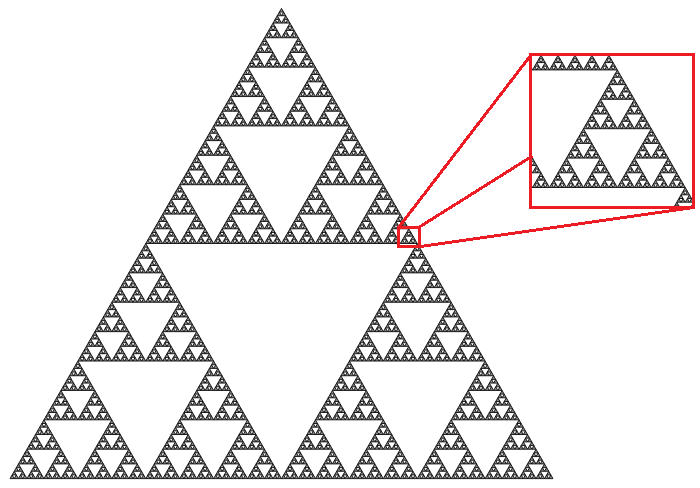
\includegraphics[width=\textwidth]{figures/fractal.png}
  \caption[The Sierpinski Triangle is an example of a fractal geometry, with a subset box illustrating the self-similar nature of the fractal.]{The Sierpinski Triangle is an example of a fractal geometry, with a subset box illustrating the self-similar nature of the fractal. The fractal dimension of the Sierpinski Triangle is 1.5849.}
  \label{fig:fractal}
\end{figure}

Fractal dimension is a useful measure of self-similarity of a two-dimensional image, and can be used to numerically quantify geometries such as coastlines, plant leaf shapes, signal waveforms, and texture patterns.  In practice, the fractal dimension can give an idea of the roughness or complexity of a particular geometry.  For example, a one-dimensional line that is bent into a zigzag shape or curved into a tight spiral starts to appear more as a two dimensional object, and its fractal dimension would increase accordingly.

%% PAGE( 3 )
In the past several decades, researchers across many fields of study have found that fractal dimension can be used to classify, categorize, and extract meaningful information contained in a digital image \cite{kucheryavski_extracting_2011}.  Fractal dimension has been used in the analysis of MRI images containing cancerous growth \cite{katsikis_fractal_2012}, in the study of electrolysis deposition \cite{nakouzi_fractal_2011}, in the classification of plant leaves \cite{du_recognition_2013}, to differentiate particle types emitted from combustion \cite{arora_morphological_2015}, and to measure bone cell activity during tooth movement \cite{adriele_silveira_new_2015}.  In all areas involving image and pattern analysis, the fractal dimension offers great potential as a novel descriptive measure.

There exist many algorithms which produce estimates of the fractal dimension of a geometry.  For well-defined geometries, the fractal dimension can often be determined analytically and/or precisely computed.  However, for natural geometries this process becomes more difficult, and different algorithms can produce conflicting estimates.  As a result, it is commonly the practice to choose an algorithm suitable for the application and use the fractal dimensional estimate to make relative comparisons between geometries, instead of using it as an absolute classifier.  It is important, therefore, to understand the strengths and limitations of the algorithm which is chosen.

The Box-Counting Algorithm (BCA) is a widely used algorithm for estimating the fractal dimension of a digital image.  It owes its popularity to its ease of implementation and the quality of its dimensional estimate on clean dimensional geometries. The BCA is well suited for calculating the fractal dimension of geometries represented in a digital image, and produces accurate estimates for images containing a clean fractal geometry.  However, the BCA is also very susceptible to image post-processing and filtering effects, such as line thickness \cite{ahammer_influence_2004}, image resolution \cite{ahammer_how_2003}, image noise \cite{reiss_noise_2015}, and non-uniform scaling \cite{soille_validity_1996}.  It is important to understand how each of these factors affect the resulting dimensional estimate in order to preserve the accuracy of relative comparisons when using the BCA.  In fact, with the multitude of factors by which the dimensional estimate of an image can be distorted, the question should be asked: "Can a good comparison of images based off the fractal dimension even be made?" 

%% PAGE( 4 )
The research presented in this paper explores the relationship between the fractal dimension estimate produced by the BCA and the variations in that estimate as noise is applied to a digital image. Two methods of adding noise, a Uniform Noise model and a Gaussian Noise model, are investigated. Simulated images of known fractal dimension and natural images which require post-processing steps are both considered.  

In an attempt to add strength to the fractal dimension estimate, data produced by the BCA's iterative measurements is analyzed to produce a metric which can be paired with the final dimensional estimate.  This metric will be referred to as a secondary key metric.  It is shown that the variance of the point-pair slope estimates produced by the BCA iterative process provides a strong secondary key metric for predicting the quality of the dimensional estimate.  In the context of this research, this variance value is a measure of the non-linearity of the point pair fractal dimension estimates, and is subsequently referred to as the slope variance of the BCA.

In the Uniform Noise model, three distinct regions are discovered that can be used to assess the quality of the dimensional estimation across the digital image test set.  The first region occurs when a very small amount of noise is introduced to a noise-free image and the dimensional estimate is shown to decrease as the slope variance increases.  The second region occurs where both the dimensional estimate and the slope variance increase in unison.  The final region occurs after the peak slope variance has been reached, and is characterized by the dimensional estimate increasing toward a maximum estimate while the slope variance decreases to zero.  It is empirically shown that dimensional estimations across a wide range of images maintain a relative ranking within each of these regions, and that understanding which region an estimate occurs may provide insight into improving classification claims based off the fractal dimension estimation.  In the Gaussian noise model, the relationship between dimensional estimate and slope variance is found to not be as useful for improving classification due to image-specific differences in dimensional content. 

%% PAGE( 5 )
While this research does not focus on improving the absolute accuracy of dimensional estimates for digital images, it shows that the relative ranking of fractal dimension estimates is preserved across a wide range of digital images regardless of the amount of uniform noise injected into an image.  This preservation of relative rankings is important in practice because there is no standardized post-processing method when it comes to handling digital images, which results in dimensional estimations which can vary greatly between studies. The research also shows that understanding in which of the three regimes a particular estimate occurs is critical when using the BCA to estimate the fractal dimension of a digital image, as dimensional estimations for similar geometries can vary greatly due to digital filtering and noise.  

% =====================================================================
% 
%      B A C K G R O U N D
%
% =====================================================================
\chapter{\textbf{BACKGROUND}}
%% PAGE( 6 )
The fractal dimension and how it is estimated for digital images using the Box-Counting Algorithm will now be explored in greater detail, followed by a summary of recent research utilizing the Box-Counting Algorithm and fractal dimension estimations.

% -------------------------------------------
%   ####
%   #   #  Background : Fractal Dimension
%   ####
%   #   #
%   ####/
% -------------------------------------------
\section{\underline{Fractal Dimension}}
A general definition of dimension was introduced by the mathematician Felix Housdorff in 1918 and is now known as the Housdorff Dimension (\(D_{h}\)).  The Housdorff Dimension is defined by the inverse relationship between the number of elemental covering units \(N\) that can completely cover a geometry and the size of this element \(r\) as: 

\begin{equation} \tag{1}
D_{h} = \frac{log(N)}{log(r)}
\end{equation}

For example, take a line of unit length.  If one were to double the length of the line, it would require double the unit length elements to cover the figure, resulting in a \(D_{h} = log(2)/log(2) = 1\).  Extending this example to a unit square consisting of sides of a unit length, doubling the length of the sides would require 4 unit square elements to cover the resulting area, yielding a \(D_{h} = log(4)/log(2) = 2\).  

The Housdorff definition holds up for integer-based dimensions, but is difficult to apply when calculating dimensions for geometries of fractal (i.e. non-integer) dimension.  It may not be possible to come up with a unit element that can completely cover a fractal geometry.  Russian mathematician Abram Besicovitch extended the Housdorff dimension equation to work on such geometries by defining a covering element of radius \(e\) and defining the minimum number of elements which could completely cover a geometry as \(N(e)\). The Housdorff-Besicovitch Dimension (\(D_{hb}\)) is generally defined as:

\begin{equation} \tag{2}
D_{hb} = \lim_{e \to 0} \frac{log( N(e) )}{log(\frac{1}{e})} 
\end{equation}  %% PAGE( 7 )
where \(D_{hb}\) is the resulting slope of the set of points in the log-log scale as \(e\)  decreases.  The fractal dimension of a deterministic fractal, defined as a fractal which is procedurally generated or mathematically defined, can be determined by the Housdorff-Besicovitch equation \cite{buczkowski_modified_1998}.

\begin{figure}[!b]
  \centering
  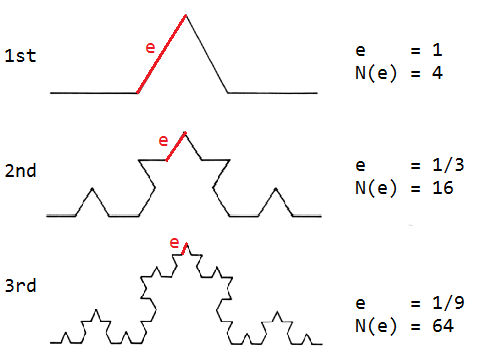
\includegraphics[width=\textwidth]{figures/kochDexample.png}
  \caption[The iterative steps showing the creation of the Koch Curve.]{The iterative steps showing the creation of the Koch Curve. With each iteration, a segment length is reduced by a factor of three while the length of the curve is increased by a factor of four.}
  \label{fig:kochDexamp}
\end{figure}

As an example, the Housdorff-Besicovitch Dimension will be calculated for the Koch Curve, which is constructed by dividing a line segment into three even segments and replacing the middle segment of the line with two segments forming two sides of an equalateral triangle (Figure \ref{fig:kochDexamp}).  This procedure is then repeated for the new set of smaller line segments, and the iteration continues indefinitely.

%% PAGE( 8 )
For the first iteration, a line segment is a size \(e = 1\) and the number of segments \(N(e) = 4\).  For the second iteration, the size of each element has been reduced by one third while the number of line segments increased by a factor of four.  Calculating the Housdorff-Besicovitch Dimension by finding the slope of points generated from the 2nd and 3rd iteration would give the following:

\begin{equation} \tag{3}
D_{hb} = \frac{log( N_{2nd}(e_{2nd})) - log( N_{3rd}(e_{3rd})) }{log( \frac{1}{e_{2nd}}) - log(\frac{1}{e_{3rd}})}
\end{equation}

\begin{equation} \tag{4}
D_{hb} = \frac{log(16) - log(64) }{log( \frac{1}{\frac{1}{3}}) - log(\frac{1}{\frac{1}{9}})}
\end{equation}

\begin{equation} \tag{5}
D_{hb} \approx 1.26186
\end{equation}
which is the fractal dimension of the Koch Curve.

Not all fractal geometries can be solved using the Housdorff-Besicovitch equation.  For complex fractal geometries, or geometries of unknown content, such as those contained in a digital image, the fractal dimension cannot be exactly solved and must instead be estimated.  The Minkowski-Bouligand (\(D_{m}\)) dimension, often referred to as the Box-Counting Dimension, defines such an estimate, and is discussed in the following section.  

% -------------------------------------------
%   ####
%   #   #  Background : Box-Counting Algorithm
%   ####
%   #   #
%   ####/
% -------------------------------------------
\section{\underline{Box-Counting Algorithm}}
The Box-Counting Algorithm is an algorithm which estimates the Housdorff-Besicovitch Dimension, and is a popular algorithm for estimating the fractal dimension of digital images.  The Box-Counting Algorithm solves for the Minkowski-Bouligand Dimension, defined as:  

\begin{equation} \tag{6}
D_{m}(Image) = \lim_{d \to 0} \frac{log( B(d) )}{log(\frac{1}{d})}
\end{equation} 

%% PAGE( 9 )
The Box-Counting Algorithm works as follows.  A uniform grid is overlaid on an image containing a particular geometry.  The size of the grid is chosen to be some width and height \(d\).  Each box in the grid is then scanned to determine if a portion of the signal geometry exists inside the box boundary.  If a portion of the signal geometry exists inside the box, it is counted.  \(B(d)\) gives the total number of counted boxes of size \(d\). As different size grid widths are chosen, the relationship between the inverse of the box size and the number of boxes counted is plotted on a log-log axis, and the slope of the line defined by these points gives the fractal dimension estimation.  The Box-Counting dimension provides the upper bound on the Hausdorff dimension \cite{camastra_data_2003}. 

When the BCA is applied to digital images, a 'countable' signal within the image needs to be defined.  This often requires some sort of digital filtering technique which converts the image into a binary set of data points being either countable or not countable.  A digital image consists of a two-dimensional array of pixels, where a pixel \(P\) can be considered a tuple containing a red \(R\), green \(G\), and blue \(B\) color intensity value, and optionally an alpha \(A\) value which defines opacity:  

\begin{equation} \tag{7}
P = (R, G, B, A)
\end{equation}

The pixel is then modified to create a countable pixel value \(P'\) which is countable or not countable:

\begin{equation} \tag{8}
P' \in \{0, 1\} 
\end{equation}

Once a threshold has been established in which countable pixels can be determined, the BCA is applied.  Scanning through each subsection of the image, one box at a time, the pixel is compared against the defined threshold.  If the pixel is countable within the box, the entire box is considered counted, and the algorithm moves to the next box.  Only one pixel within a box needs to be considered countable for the entire box to be considered countable.  Figure \ref{fig:boxcount} shows an image which has been overlain with two different widths of boxes, and the counted boxes are highlighted. 

%% PAGE( 10 )
Choosing several values of \(d\) produces a set of dimensional estimates that should form a linear relationship on a log-log scale.  The fractal dimension estimate is the slope of these points.  For pure fractal geometries, the BCA produces a set of estimates which are stable at any size of grid width chosen. However, there are many factors that can influence the fractal dimension estimate, especially when dealing with digital images.

\begin{figure}[!b]
  \centering
  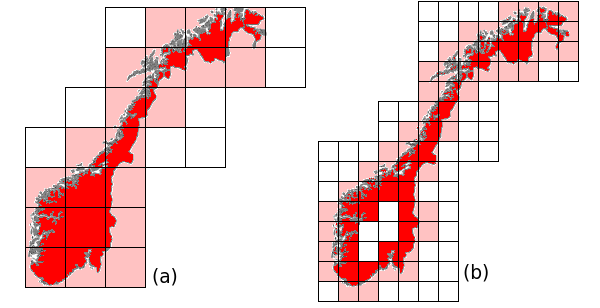
\includegraphics[width=\textwidth]{figures/boxcount_fig.png}
  \caption[An example of counted boxes on the coast of norway]{An example of counted boxes on the coast of norway, where the box width is some length \(d\) (a) and \(d/2\) (b).}
  \label{fig:boxcount}
\end{figure}

Because a digital image consists of a finite set of pixels, infinite resolution on fractal geometries cannot be represented.  Eventually any self-similarity present in a geometry will be destroyed by the finite pixel resolution (see Figure \ref{fig:pixelation}).  Although it has been shown that different image resolutions can still produce fractal dimension estimations that are relatively stable \cite{ahammer_how_2003}, the dimensional estimates are skewed for very small box widths.  Also, this requires that an image be of sufficiently large size as to allow several differing size grid widths to be processed.

\begin{figure}[!b]
  \centering
  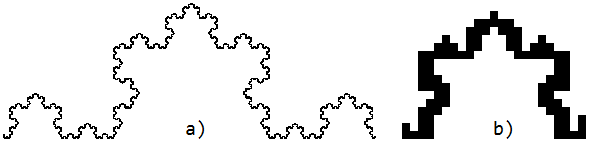
\includegraphics[width=\textwidth]{figures/pixelation_fig.png}
  \caption[An example of the resolution limitations of a digital image.]{An example of the resolution limitations of a digital image.  Here we have a digital representation of the Koch Snowflake (a) and a zoomed-in example of a leaf from the Koch Snowflake (b) showing pixelization and signal loss.}
  \label{fig:pixelation}
\end{figure}

%% PAGE( 11 )
Non-simulated digital images are subject to many types of distortions that can affect the quality of the image content.  Images which are scanned are subject to loss of signal due to converting analog signal to digital.  Digital cameras are subject to electronic noise which can manifest down to the component and sensor levels.  Digital filters can be implemented to attempt to decrease artifacts such as noise, but it has been shown that post-processing filters also influence the fractal dimension estimate. Gaussian noise, which can be injected as a noise blurring filter, has been shown to cause increases in dimensionality estimates, and to increase the fractal dimension estimates of lower-dimensional geometries more strongly than higher dimensional geometries \cite{reiss_noise_2015}.  Line thickness, which can be an artifact of edge-detection image filtering algorithms, has been shown to be directly proportional to the fractal dimension estimate produced by the BCA as well \cite{ahammer_influence_2004}.  

The fractal dimension measurements of digital images are weakened by linear transformations of pixel intensity (the grey-scale pixel values), and by transformations of scale, such as magnification along a single axis of an image.  Therefore, when using fractal dimension as a quantitative measure for image comparison, it is important that image intensities and scaling are taken into consideration. \cite{soille_validity_1996}

%% PAGE( 12 )
The BCA will always yield an estimate, and to the unaware user, this estimate may seem like a valid value.  Due to the large number of factors that can influence this number, it is critical to understand these influences in order to add validity to any claims based on BCA estimate data.  The research provided here attempts to add to the body of work that explores how external processing effects can be interpreted and handled.  It will be shown that even small amounts of additive noise can produce dimensional estimates deviating as much as 30\% from the baseline dimensional estimate.

% -------------------------------------------
%   ####
%   #   #  Background : Literature Review
%   ####
%   #   #
%   ####/
% -------------------------------------------
\section{\underline{Box-Counting Algorithm Refinements}}
There have been many studies reviewing the validity of the Box-Counting Algorithm and methods in which to improve the accuracy of BCA estimations.  These studies have highlighted the importance of post-processing techniques and parameter selection.

% Improvements or Studies
One component that influences the BCA estimation is the selection of a proper set of operating parameters.  Choosing a good set of grid widths can play an important factor in the dimensional estimation result.  Meisel and Johnson measured the amount of points required for convergence using the BCA \cite{meisel_convergence_1997}.  Tolle et al. used clustering algorithms to find the minimum size of a covering element given a desired number of counted elements.  The results of this research improved upon the upper bound of the fractal dimension estimate, but at the expense of several orders of magnitude the computational cost.  This approach predicts more stable fractal dimension estimations on higher dimensional data sets \cite{tolle_suboptimal_2003}.

Other research focused on improving the fractal dimension estimation itself.  A study by Buczkowski et al. attempted to better define the initial conditions of the BCA to diminish the influence of edge effects \cite{buczkowski_modified_1998}.  Setting an origin for the grid in the center of an image, and removing 'plateau' grid width sizes (grid widths that produce the same number of boxes counted), this approach removed some of the variability in the BCA fractal dimension estimation.  However, this study did not show comparative results to the non-modified box-counting method, and this method was optimized for non-natural, carefully generated digital fractal images.  Balghonaim and Keller used a maximum likelihood estimator to improve upon the BCA dimensional estimation \cite{balghonaim_maximum_1998}.  Spodarev et al. paired the calculation of fractal curvature with the fractal dimension estimate to produce a more robust classification of fractals \cite{spodarev_estimation_2015}.

\section{\underline{Box-Counting Algorithm in Image Processing}}
%% PAGE( 13 )
% Examples used in research
There are many examples of fractal dimension analysis being used for classification and recognition purposes across a wide variety of disciplines.  Sarkheil and Rahbari used the BCA dimensional estimation to classify modified natural starch into categories which represented good and poor suitability for use in polymers \cite{sarkheil_fractal_????}.  Du et al. combined fractal estimates produced from the BCA with a K nearest neighbor classifier to develop a method to recognize and classify plant leaf images  \cite{du_recognition_2013}.  Arora and Jain used the BCA as one of several methods to attempt to classify particles emitted from combustion ovens when burning different types of fuel \cite{arora_morphological_2015}.  Katsikis used the BCA along with the Hand and Divider method and a modified Differential Box-Counting Algorithm, which estimated the grey scale intensity of an image as a third dimensional parameter, and applied these algorithms to analyze biomedical images \cite{katsikis_fractal_2012}. Focusing on MRI scans containing areas of cancerous growth, the goal was to attempt to use a fractal dimension approach to isolate the cancerous regions.

Several recent orthodontic studies have used fractal dimension to recognize patterns in bone structures. Amer et al. used the BCA to estimate the fractal dimension of the trabecular bone, which is a spongy bone structure. Starting with an image size of 100x100 pixels, then using multiple stages of filtering (including a Gaussian filter) to produce a final outline, and selecting a set of box widths down to a 2-pixel size, this study qualifies as one in which many factors are likely influencing the final calculated dimensional estimate.  The resulting dimensional results were very close to one another, yet the paper claims that a normal, healthy trabecular pattern has a fractal dimension of 1.5 \cite{amer_anatomical_2012}.  A second study published by Adriele et al. used fractal analysis via the BCA to evaluate osteoclastic activity induced by orthodontic loading.  This research successfully used the BCA and fractal dimension to measure a single linear boundary which grew in complexity as osteoclastic activity occurred, producing results that had previously only been achieved by manual counting, which was a laborious and error-prone approach \cite{adriele_silveira_new_2015}.

%% PAGE( 14 )
% -- classification type
Additional research includes a study conducted by Nakouzi and Sultan which used the BCA dimensional estimates to categorize deposition by electrolysis in a two-metal solution which produced fractal-like patterns depending on the level of voltage applied \cite{nakouzi_fractal_2011}.  Finally, a study produced by Szkiva et al. compared the fractal dimensions of laser-irradiated vanadium surfaces under different applied liquids \cite{szkiva_fractal_2013}. The image samples used in this research were post-processed with a threshold filter which used as a threshold the midpoint value between the maximum and minimum intensity pixel in the image. The results of this study report fractal dimension estimations that were very similar (within a tenth) to one another, yet the author makes the claim that fractal dimension estimations as they proposed are a valid form of classifier in this application. As data produced in this paper will highlight, the fractal dimension estimation can change drastically when using a threshold filter with varying levels of threshold parameter.

% -- other novel uses
Fractal dimension is not only used as a classifier of images.  Several published articles highlight approaches that use the fractal dimension to enhance other areas of image analysis.  Novianto et al. presents an algorithm to estimate local fractal dimensions in textured images, focusing on 3x3 pixel subsections of the image, and then using the resulting fractal dimension map as an alternate approach to creating image segmentation maps \cite{novianto_near_2003}.  Uemura et al. suggested modifications to the BCA box scanning method and subsequent fractal dimension estimations to improve upon edge detection capabilities in MRI images of brain scans  \cite{uemura_generation_2000}.

% =====================================================
% 
%      M E T H O D S
%
% =====================================================
\chapter{\textbf{METHODS}}
%% PAGE( 15 )
An overview of the project is discussed in this section, followed by a detailed methodology of each major component which is illustrated in Figure \ref{fig:process}.

The process starts with a digital image, which can be a full-color natural image, or a carefully designed artificial geometry.  A digital image is represented as a two dimensional matrix of pixels, where a pixel comprises a tuple of values representing the intensity of red, green, and blue light required to display a particular color. A white pixel in an image is the result of the red, green, and blue light intensity values being uniform and maximum, whereas all three values of a black pixel have zero intensity.  In a gray-scale image, the red, green, and blue intensity values are the same for each pixel.  It is the mixing of these three color elements which produces the full range of colors in a digital image.  In a 24-bit color image, each of the three color values exist in the range 0-255.

The Box-Counting Algorithm requires each pixel of an image to be in one of two states: countable or not countable.  These states can be represented by the two pixel intensity values black and white, where a black pixel represents a countable portion of the image, and a white pixel represents a non-countable portion of the image.  For processing purposes, it is possible to take the set of red, green, and blue color values of a pixel and condense them down to be either black or white.  If a test image is artificially created, it might already exist in this state.  For example, an image of a circle geometry would have a black circle on a white background, where the black perimeter of the circle represents the countable portion of the image.  This type of image would not require a post-processing step, as it already consists purely of white and black pixels and is ready to be handled by the box-counting algorithm. For non-generated real-world images, a post-processing filter needs to be applied in order to convert a full-color or gray-scale image into a pure black and white image.  A post-processing filter in the context of this research represents an algorithm that intelligently converts a set of red, green, and blue color values into either a black or white representation of a pixel.

\begin{figure}[!b]
  \centering
  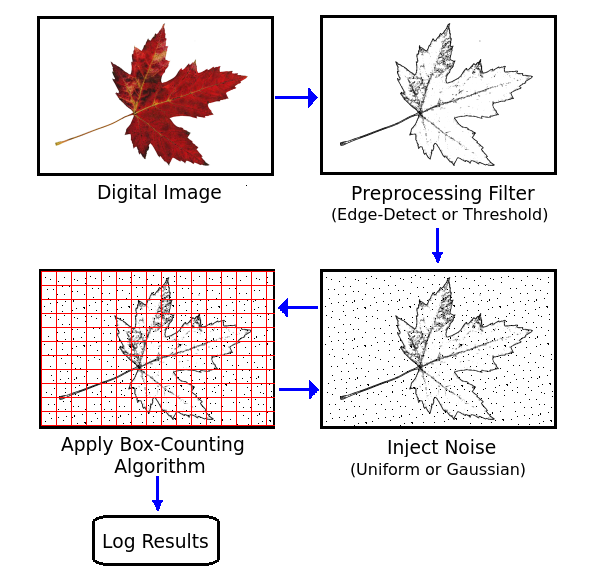
\includegraphics[width=\textwidth]{figures/process.png}
  \caption[The processing pipeline which takes a digital image and produces a set of fractal dimensional estimates across a range of noise levels.]{The processing pipeline which takes a digital image and produces a set of fractal dimensional estimates across a range of noise levels.}
  \label{fig:process}
\end{figure}

Once a post-processing filter has been applied, it is time to begin the iterations of adding noise to the image, and then running the noisy image through the Box-Counting Algorithm.  The two noise models tested in this research are Uniform Noise and Gaussian Noise.  Each iteration of the Box-Counting Algorithm produces data that is written to a data log file for later analysis.  More noise is then added and the process continues until we fully obfuscate the original image due to noise. 

%% PAGE( 17 )
This project required a large computational effort to complete, with hundreds of hours of processing time required to run all simulations presented.  The processing pipeline had a computational cost on the order \(O(n^{8})\), where \(n\) is any of the possible pipeline parameters that are scalable, and required a multi-core environment to complete the simulations within a reasonable time frame.  The pseudocode for this pipeline is shown in Figure \ref{fig:code_pipeline}.

% Begin a new figure
\begin{figure}
% Make this figure a code block
% More info here: https://en.wikibooks.org/wiki/LaTeX/Source_Code_Listings
\begin{lstlisting}
for each image in image_set:
    for each filter in preprocessing_filter_set:
        for each noise_model in noise_model_set:
            for each seed in noise_seed_set:
                for each noise_level in noise_level_set:
                    for each box_size in box_grid_size_array:
                        for each row in image:
                            for each column in image:
                                boxcount_pixel()
\end{lstlisting}
% end of code block
\caption{Pseudocode illustrating the computational scaling cost of this research.}
\label{fig:code_pipeline}
\end{figure}

% -------------------------------------------
% 
%     Methods : Development Environment
%
% -------------------------------------------
\section{\underline{Development Environment}}
All of the algorithms used in this research were implemented in the Python 3 language.  The BCA was implemented from scratch, and the edge detection and threshold digital image filters were developed in-house, along with all data processing and aggregation code.  All data plots were implemented using the Matplotlib library for Python.

The Python Numpy module was used to increase efficiency of matrix manipulations.  The Python module Scipy was used for its Gaussian blur image filter.  The post-processing image filtering algorithms were originally written to work with BMP formatted images, but for efficiency reasons the input image format was switched to PNG formatting which was compatible for opening and processing using the Numpy library. 
%% PAGE( 18 )
The code base was regularly pushed to a Github repository in order to allow for code development from multiple locations.  A Dell Inspiron 15 laptop (Intel Core i7 processer, 2.00 GHz, 8 GB RAM) served as the primary development and debugging hardware running Ubuntu through Oracle VM VirtualBox, while a Unix cluster consisting of 256 cores was used to process the majority of simulations.  On the Dell Inspiron hardware, the typical run time to perform the BCA on a single noise seed using the Uniform Noise model took approximately 9 minutes, while the Gaussian Noise model took approximately 23 minutes.

In order to standardize the test image set size and formatting, images were initially created and cropped using the freely available KolourPaint software (\url{http://kolourpaint.en.uptodown.com/ubuntu}).  Many of the figures found in this document were also created using the KolourPaint software.


% -------------------------------------------
% 
%     Methods : Image Selection
%
% -------------------------------------------
\section{\underline{Image Selection and Creation}}
The complete set of images used in this research are shown in Appendix B.  Several key factors played a role in selecting this image set.  It was important to select a set of images that spanned the possible dimensional range contained within a two-dimensional image, therefore figures with known dimensional geometries spanning from 1 to 2 dimensions were selected.  A set of pure fractal geometries with well-defined fractal dimensions were chosen to validate the implemented BCA and to set a baseline for comparison when looking for relationships with secondary keys.  These images include the line, circle, Koch Snowflake, and fifty50 images.  The canopy image was included as it contained thick lines and fractal properties in juxtaposition to the thinly-lined fractal set.

In natural images, one would expect a mixing of dimensional signals contained in the image.  Therefore a simulated image containing mixed geometries was added to the image set.  The Koch Snowflake was intersected by 3 single pixel width lines to serve as an example of pure dimensional geometries interacting with one another.

%% PAGE( 19 )
Coastlines and leaf perimeters are both objects in nature that exhibit strong fractal qualities.  A rendered coastline of Norway was included in the data set, as well as a natural image of a leaf over a white background.  The coastline of Norway did not require any image filtering as it already consisted of only black and white pixel data, but the leaf image was a full 24-bit color image and required post-processing.  Therefore, choosing an image of a leaf strongly contrasted by a white background allowed for an edge-detect filter to highlight the leaf perimeter and minimized other distorting effects that might bias the BCA results.

A blank image containing only white pixels was included to allow simulation of the BCA on a purely Uniform Noise model.  This image allowed comparisons to be made between all other image simulations to the noise baseline simulation.

Finally, a natural image was selected that contained no apparent dimensional content and represented a challenging image in which to apply a filter.  A full-color natural image of an owl camouflaged against a tree was selected as it contained multiple objects within (the owl and the tree), but displayed no obvious filtering choice to best expose the embedded objects.  This image was processed using both an edge detection filter and a threshold detection filter.

An image size of 2100 pixel width by 1800 pixel height was chosen to provide adequate pixel resolution, which allowed a wide range of grid sizes to be used.  These image dimensions facilitate the use of a large set of box sizes which fit evenly within the image bounds, avoiding the case where boxes extend outside the bounds of the image size.  This image ratio also allowed for the inclusion of a large variety of image content.

The blank image, line image, circle image, and fifty50 images were created using the KolourPaint application.  Line and circle widths were set to 1 pixel to minimize line width BCA distortions.  The \textit{fifty50} image was created by selecting half of the image to be purely black and leaving the other half completely white.  The Koch Snowflake image was obtained from the Wikipedia website under the common use license and chosen due to its sufficiently large size and image resolution.  The Koch Snowflake intersected by three lines was created using the KolourPaint application to apply three 1-pixel width lines to the above Koch Snowflake image.

%% PAGE( 20 )
The image of the coast of Norway was obtained from \url{http://www.ginkgomaps.com/en/rl3c_no_norway_map_plaindcw_ja_mres.jpg} and was manully manipulated using the KolourPaint software to remove the map borders and text, to 'paint' the grey interior to be white, and converted to PNG format as a purely black and white image.  The image of the leaf was obtained from \url{https://people.rit.edu/~andpph/photofile-misc/Leaves-in-Fall/}, and chosen due to its large resolution and stark white background, which allowed for clean post-processing and filtering.  The image of the owl was obtained from \url{http://www.wimp.com/animalcamo/} and chosen because of its interesting and unknown geometries, as well as for its high resolution.

Two image file formats were used to create the input files for this research.  Originally, a BMP file format was chosen due to its uncompressed representation of pixel data and its ease of parsing for the manual creation of post-processing filters.  A BMP class was built in-house to convert the raw image into a clean two dimensional array.  The edge detection and threshold filters were then written to interface with the BMP image data.  When creating the edge detection and threshold detection filtered images used in this research, the leaf image and owl image were saved in BMP image format and then the filters were applied, creating a set of post-processed images ready for the BCA.  It was later decided to use the Matplotlib image library to allow for more efficient processing and converting of image data into a two-dimensional filtered matrix of pixels, so the entire set of images was converted to the PNG image format, which also supports uncompressed image pixel data.

The \textit{owl} image and \textit{fallleaf} image required post-processing prior to analysis by the BCA.  The \textit{fallleaf} image offered a clean fractal-like perimeter geometry, and the edge-detection filter was the obvious choice to highlight the perimeter portion of the image.  A set of 15 images was created by processing the \textit{fallleaf} image using an edge-detection filter with thresholds ranging from 5 to 75, in steps of 5.  The filtering algorithm required a BMP image format as input and produced a BMP image formatted filtered output image, which was then converted to PNG format for use with the BCA.  

%% PAGE( 21 )
The \textit{owl} image did not suggest an optimal filtering algorithm, so both the edge-detection filter and threshold filter were used.  A set of 15 images was created by processing the \textit{owl} image using an edge-detection filter with thresholds ranging from 5 to 75, in steps of 5.  A set of 20 images was created by processing the \textit{owl} image using a threshold filter with thresholds ranging from 10 to 200, in steps of 10.  Each of these sets of images were initially formatted as BMP images and were converted to the PNG format after filtering was complete.

% -------------------------------------------
% 
%     Methods : Image Processing Filters
%
% -------------------------------------------
\section{\underline{Image Processing Filters}}
Two simple post-processing filters were created to convert a natural color or gray-scaled digital image into a black and white image ready to be handled by the Box-Counting Algorithm.  These filters were written in-house and designed to work with a BMP image type, although they could be modified to work with any two-dimensional array of pixel values.

The first filter created is an edge-detection filter.  This filter scans over each row of pixels in a two-dimensional image and compares the pixel intensity to that of neighboring pixels.  The pixel intensity is defined as the average of the red, green, and blue color intensity value of a single pixel, which for an image with 24-bit color depth, each color intensity value is in the range of 0-255, meaning the resulting intensity of a pixel would also be in the range of 0-255. Starting at the top corner of an image, scanning left to right across a row of pixels, then proceeding to the next row underneath, each pixel intensity is compared with its right and bottom neighboring pixels.  If the intensity differential is greater than a set threshold value, which is a parameter of the filter function, the original pixel is turned into a black 'countable' pixel.  Otherwise it is turned into a white 'uncountable' pixel.   

%% PAGE( 22 )
The edge-detection filter converts to black pixels the areas of an image with large intensity gradients, which highlights the edges of different regions of an image.  For images such as a darker leaf resting on a lighter background, the edge-detection filter can successfully highlight the perimeter of a leaf as a black outline, while the inner and outer surfaces are converted to white (see Appenix B, Figure \ref{fig:20fallleaf_png}). For images without apparent boundaries, the results can be unpredictable (Figure \ref{fig:edfilter}).  Regardless of image content, the edge-detection filter is useful for pulling out the boundary geometries of contrasting figures contained in a digital image.

\begin{figure}[!b]
  \centering
  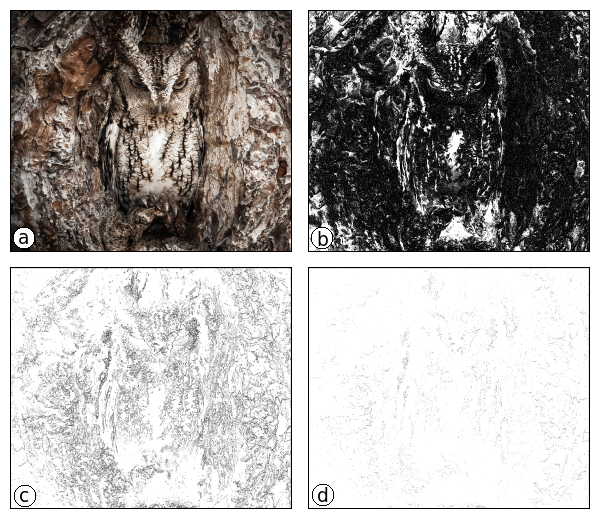
\includegraphics[width=\textwidth]{figures/owl_ed.png}
  \caption[The edge-detection filter on a natural image of an owl]{The edge-detection filter on a natural image of an owl (a), at threshold levels of 5 (b), 40 (c), and 75 (d).}
  \label{fig:edfilter}
\end{figure} 

%% PAGE( 23 )
The second filter created is a threshold filter.  This filter also iterates over each individual pixel in an image, but instead of comparing pixel intensity to that of a pixel's neighbor, each pixel's intensity is compared to a global threshold value which is passed to the filter as a parameter.  All pixels with an intensity greater than that of the defined threshold value are converted to black, while those less than the threshold value are converted to white. As a result, areas of higher intensity are interpreted as signal, leaving lower intensity regions as background.

The threshold filter is used for highlighting solid regions inside a geometry, and offers an alternative filtering method to the edge-detection filter.  For particular pattern recognition, a threshold filter may offer a valid alternative to highlighting the signal of interest inside an image.  An example of the threshold filter on the owl image can be seen in Figure \ref{fig:threshfilter}.

\begin{figure}[!b]
  \centering
  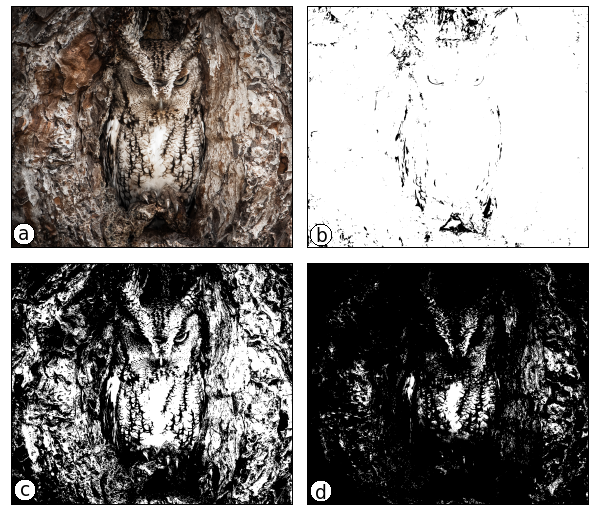
\includegraphics[width=\textwidth]{figures/owl_thresh.png}
  \caption[The threshold filter on a natural image of an owl]{The threshold filter on a natural image of an owl (a), at threshold levels of 10 (b), 100 (c), and 200 (d).}
  \label{fig:threshfilter}
\end{figure} 

Both filters developed for this research operated on BMP formatted images as input and produced black and white BMP formatted output images.  These images were then converted to the PNG format prior to BCA analysis using the KoulorPaint software.  No black and white image pixel data was lost or corrupted during the conversion process between these two image format types.

% -------------------------------------------
% 
%     Methods : Selection of Noise Models
%
% -------------------------------------------
\section{\underline{Selection of Noise Models}}
Two noise models were selected for investigation in this study.  The first is a uniform noise model.  In this model, we consider a black and white digital image where the black pixels constitute the interesting signal.  Uniform noise is injected onto the image in the form of flipping the color of a particular pixel.  A non-signal pixel is changed to black in the presence of noise, and a signal pixel is changed to white in the presence of noise.  

\begin{figure}[!b]
  \centering
  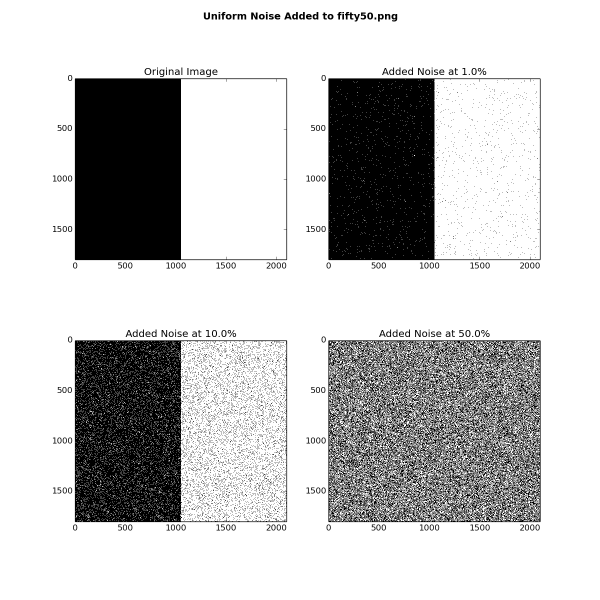
\includegraphics[width=\textwidth]{figures/uniform.png}
  \caption[The effects of adding uniform noise to an image.]{The effects of adding uniform noise to an image.}
  \label{fig:uniform}
\end{figure}

%% PAGE( 24 )
The Uniform Noise Model was implemented by creating a two-dimensional array of seeded random floating point numbers in the range [0,1). This two-dimensional noise array matched the dimensions of the two-dimensional image array.  To achieve a specific percentage of Uniform Noise added, the desired percentage number served as a threshold value, where any element in the noise array falling below the threshold value caused the corresponding element in the image array to be 'flipped' from black to white or vise-versa.  For example, if 10\% uniform noise were to be injected into an image, then every (x,y) element in the noise array with a value less than 0.10 would trigger the corresponding (x,y) element in the image array to be flipped (Figure \ref{fig:uniform}).

%% PAGE( 25 )
For a given image in the test image set, uniform noise was injected repeatedly starting at 0.0001\% and increasing up to 50\%.  To ensure that the pixels affected at lesser percentages carried over to higher percentages, the randomize function was given a starting seed value which was held constant over each iteration of additive noise.  Therefore, whether 1\% or 10\% uniform noise was injected into an image, both cases started injecting from the initial image state, and all pixels affected in the 1\% case would also be affected in the 10\% case for a given starting seed.

%% PAGE( 26 )
The second model investigated was a Gaussian noise model.  Unlike the Uniform noise model, where each pixel in the image has an equally probable chance to be flipped, the effects of Gaussian noise are localized around the signal itself.  Gaussian noise is controlled by a sigma value which introduces a blurring effect to a digital image.  The Gaussian filter inside the Scipy module was chosen as the implementation of this model, and the sigma value was adjusted from a value of 1 to 1000.

The Scipy Gaussian filter results in a gray-scale blurring of pure black and white images, and a particular value of sigma would produce the same filtered result each time the filter was called.  In order to convert the gray-scale filtered image back into a probability-based black and white noisy image, the gray-scale intensity of a pixel was normalized into the probability in which the pixel would become black. For a 24-bit image, pixel grey-scale values exist in the range [0,255].  This range was then interpreted to represent a 0\% to 100\% chance of being converted into a white pixel.  A dark-grey pixel with a normalized gray-scale value of 0.01 would only have a 1\% chance of being turned white, while an light-grey pixel with a normalized gray-scale value of 0.99 would have a 99\% probability of remaining white (Figure \ref{fig:gaussian}).

\begin{figure}[!b]
  \centering
  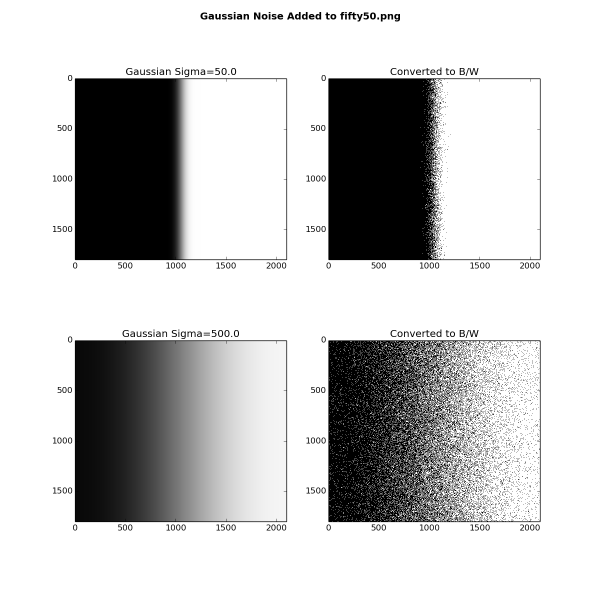
\includegraphics[width=\textwidth]{figures/gaussian.png}
  \caption[The effects of adding Gaussian noise to an image.]{The effects of adding Gaussian noise to an image.}
  \label{fig:gaussian}
\end{figure}

Similar to the Uniform Noise model, the Gaussian model also used a seeded random function to ensure that each subsequent iteration of the BCA would produce the same noise characteristic.  Each test image analyzed in this research was analyzed using a set of 100 distinct random seeds, and the mean results of these tests were used for plotting an analysis.  The seed values used for both the uniform and Gaussian noise case were the numbers 1 through 100.

% -------------------------------------------
% 
%     Methods : Secondary Key Metric
%
% -------------------------------------------
\section{\underline{Selection of Secondary Key Metric}} The Box-Counting Algorithm will always produce a dimensional estimate value, and does not by default provide any information regarding the quality of this estimate.  Due to the multitude of factors which can distort a dimensional estimation (discussed in detail in the previous chapter), a dimensional estimate must be interpreted carefully.

%% PAGE( 27 )  /  %% PAGE( 28 )
The BCA estimates the fractal dimension at different magnitudes of scale, and the slope produced by the full set of data points is used as the final estimate.  Using the linearity of this set of data points as a quality indicator seemed like a good measure of the quality of the final dimensional estimate.  Therefore, these data points were analyzed to determine a secondary key metric to use as a quality indicator for the fractal dimension.  Four algorithms were tested using the local slope values produced by neighboring sets of points produced by the BCA iterative process.  These localized slopes are referred to as point-pair slopes.  The four algorithms explored were the variance of the point-pair slopes, the population variance of the point-pair slopes, the sum of the differences between the point-pair slopes, and the sum of the central differences between the point-pair slopes.

The variance of the point-pair slopes was calculated using the Numpy variance function \(var()\), which is equivalent to the following equation:

\begin{equation} \tag{9}
var() = \frac{\sum{(x-\bar{x})^{2}}}{N-1}
\end{equation}
where \(x\) is a point-pair slope, \(\bar{x}\) is the mean of the point-pair slope set, and \(N\) is the total number of point-pair slopes.  Similarly, the slope population variance, \(SPV\), was calculated using the following equation:

\begin{equation} \tag{10}
SPV = \frac{\sum{(x-\bar{x})^{2}}}{N}
\end{equation}

The sum of the slope differences was calculated using the following equation, where \(x_{n}\) is a point-pair slope, \(x_{n+1}\) is the next sequential point-pair slope, and \(N\) is the total number of point-pair slopes: 

\begin{equation} \tag{11}
SD = \sum_{n=1}^{N-1}|x_{n} - x_{n+1}|
\end{equation}

The sum of the central differences, SCD, was calculated using:

\begin{equation} \tag{12}
SCD = \sum_{n=1}^{N-1}|x_{n}^{'} - x_{n+1}^{'}|
\end{equation}
where \(x_{n}^{'} = (x_{n} + x_{n+1})/2\) represents the central difference between point-pair slopes.

%% PAGE( 29 )
All four secondary key metrics were calculated for each test image based on the averaged point-pair slope data aggregated from 100 uniquely seeded simulations.  For each key metric, the standard error was also calculated.

% -------------------------------------------
% 
%     Methods : Box-Counting Algorithm
%
% -------------------------------------------
\section{\underline{Implementing the Box-Counting Algorithm}}
The BCA was implemented from scratch in Python 3.  The BCA requires two input parameters, the first being a two-dimensional matrix of binary data, representing either a countable or non-countable entity, and the second parameter being a set of grid widths on which to generate the box sizes to be tested for countability.  

The two-dimensional matrix was created by taking a PNG formatted image and reading it into a three-dimensional matrix, where two dimensions held the row and column pixel data for the image, and the third dimension representing the pixel values for red, green, blue, and alpha channel.  The alpha channel was then stripped, and the resulting red, green, and blue values were averaged to obtain a gray-scale intensity value.  Since all of the images in the test set were either constructor or pre-filtered to consist of only black and white pixel data, the average of the red, green, and blue pixel intensities always resulted in either a 0 (representing no intensity, or a black signal) or 255 (representing all intensities, or a white signal).  These values were then normalized into a binary 0 or 1 value, where 0 represented a countable pixel element, and 1 represented a non-countable pixel element.  Although representing a countable pixel as a 0 might not seem intuitive, programmatically it made sense since the intensity of a black pixel is also 0.

Several considerations taken when choosing a set of grid widths for the BCA.  In order to achieve an accurate dimensional estimate, the BCA requires a selection of box widths which cover the image at as many scales as possible.  The scale of the boxes had a lower limit of 1 pixel, as this was the smallest resolution possible in a digital image.  The upper limit was set by the dimension of the image itself.  Resolution at the very small scale (1 pixel) would not yield an accurate estimate because at this resolution all complexity within the image is lost and we have reached the noise floor of the image.  Likewise, a grid width set at the size of the image would not yield a good estimate, as it would always be considered a countable box.  

%% PAGE( 30 )
Another consideration was at what scale to select the grid sizes.  The larger the quantity of box sizes included in the set could increase the accuracy of the BCA estimate, although at the expense of computational requirements.  Choosing a grid width at increasing orders of magnitude would offer the best overall estimate of the global fractal dimension, since a true fractal geometry exhibits the same complexity over all scales. The grid selection should therefore attempt to cover the maximum number of ranges from smallest reasonable box width to largest reasonable box width.

Finally, one had to consider whether to choose a set of box sizes that produced grids that would evenly fit inside the image dimensions, or allow grid sizes to extend outside of the bounds of the image.  An overlapping grid would not necessarily produce incorrect results, as one could imagine for an image containing a fully contained geometry, that any pixel outside the image dimension would automatically be considered not countable.  However, for images containing unknown dimensional content, which could exist up to the image borders, an overlapping grid size might produce undesired edge effects.  Therefore, for this research, a set of grid sizes which cleanly fit inside the image dimensions were selected.  

An image size of 2100 x 1800 pixels allowed for the following grid sizes:  3, 5, 10, 20, 30, 50, 100, 150, and 300.   This set of box sizes allows for a grid which precisely fits within the bounds of the digital image, includes grid sizes ranging over 2 orders of magnitude, and offers enough data points to analyze for secondary key metrics.

%% PAGE( 31 )
The implementation of the BCA in Python takes as parameters the two-dimensional matrix of binary data and the array of grid sizes.  For each grid size, the two-dimensional matrix is divided into \(n\) x \(n\) width subsections, where \(n\) is the current grid size.  The subsection of the array is then scanned in search for a countable element (\(element = 0\)).  Once a single countable element is found, the algorithm stops scanning the current subsection and moves to the next in order to improve computational costs.

Once all the boxes are counted for a particular grid size, the total number of counted boxes is written to a log file, along with information containing the image name, grid width, and noise seed, for later processing.
% -------------------------------------------
% 
%     Methods : Data Aggregation
%
% -------------------------------------------
\section{\underline{Data Aggregation}}
Data produced by the Box-Counting Algorithm was written to output files for later processing.  A separate data log was created for each unique image and noise seed pairing.  For this research, the test image set contained the blank image used for baseline uniform noise analysis, 8 simulated images, 15 images generated from the \textit{fallleaf} image and edge-detection filtering, 15 images generated from the \textit{owl} image and edge-detection filter, and 20 images generated from the \textit{owl} image and threshold filtering, for a total of 59 images. This image set was simulated under both the uniform and Gaussian noise models using 100 seeds for each model, producing 11700 data logs.

Each of these data logs included both reference data describing the parameters of the simulation and calculated data.  The reference data included items such as image name, grid width, noise model, noise seed, and a time-stamp for the simulation.  The calculated data included the number of boxes counted at each grid size and at each level of input noise strength.  

Before generating and analyzing the data, each set of 100 data logs (representing the 100 unique noise seeds) for an image and noise model pairing was aggregated, secondary metrics were calculated along with each metrics' standard error, and the aggregated logs were written to output files.  Therefore, a set of 117 aggregated data logs were produced containing the final results for each simulated set.  The entire set of data logs and aggregated data logs are publicly available at the following URL: \url{https://github.com/mcm7f/thesis/tree/master/logfiles}.

% =====================================================================
% 
%      R E S U L T S
%
% =====================================================================
\chapter{\textbf{RESULTS}}
%% PAGE( 33 )
The results produced by this research are presented in this chapter.  These results include secondary key relationships, uniform noise results, and Gaussian noise results. Additional figures for the uniform noise simulations are presented in Appendix C, and additional figures for the Gaussian noise simulations are presented in Appendix D.

% -------------------------------------------
% 
%     RESULTS : Secondary Key
%
% -------------------------------------------
\section{\underline{Secondary Key Results}}
The relationship between fractal dimension and the following four secondary keys were explored under the uniform noise model: Slope Variance, Population Slope Variance, the sum of the differences of the slope pairs, and the sum of the central differences of the slope pairs.  The profile of these metrics are shown in Figure \ref{fig:keyComparison} for the \textit{kochSnowflake} image.  

The simulated images in the image test all produced a Slope Variance curve with a similar profile.  The slope variance started near zero at low input noise values, increased in value up to a single local maximum value, then decreased back toward zero as the input noise approached 50\%.  The sum of the difference and sum of the central difference plots did not produce a strong curve profile that carried over from one image to the next.  The sum of the difference key metrics produced plots containing several local minimum and local maximum values.

The secondary key comparison data was gathered from aggregating the data logs created from BCA simulations using 100 different uniform noise seeds.  The standard error was computed for each secondary key, but were too small to be visible when plotting the results.  Typical standard error values were less than \(1e10^{-4}\). Only slope variance was calculated for the Gaussian Noise case.

\begin{figure}[H] % Lock this figure in by hand or else all figures drift downstream
  \centering            % Don't mess with this scale!
  \frame{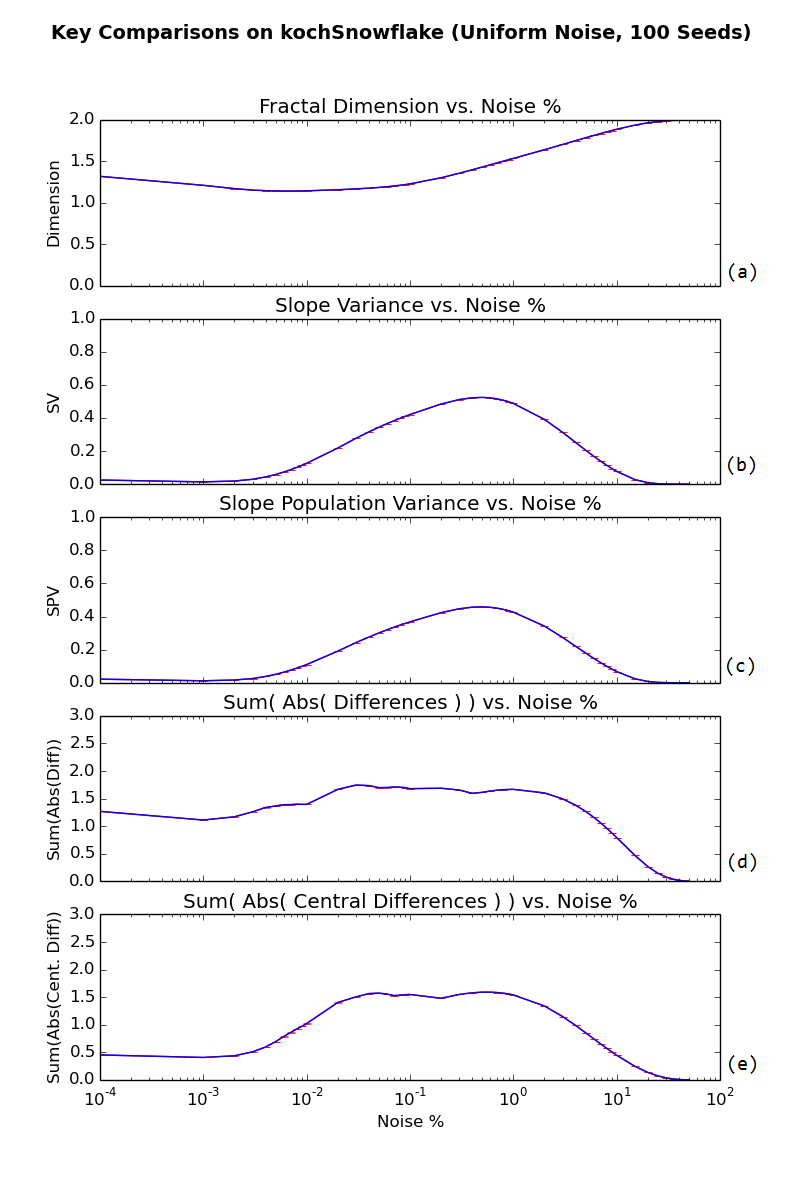
\includegraphics[scale=0.7]{figures/kochSnowflake_uniform_keyComparisonsFig.png}}
  \caption[Several secondary key relationships with the Fractal Dimension]{Several secondary key relationships with the Fractal Dimension (a).  The Slope Variance (b) exhibits the strongest relationship across the entire image test set, followed by the Slope Population Variance (c).  The relationship of other keys were not as apparent across the image set (d), (e).  The standard errors are also plotted, but are so small as to be negligible here.}
  \label{fig:keyComparison}
\end{figure}

% -------------------------------------------
% 
%     RESULTS : Box-Count Algorithm
%
% -------------------------------------------
\section{\underline{Box-Counting Algorithm}}
%% PAGE( 34 )
The Box-Counting Algorithm was implemented in-house, and therefore the results of the algorithm needed to be validated.  Several known dimensional geometries were tested and the fractal dimension estimates were compared against the mathematically defined fractal dimensions (Table \ref{tab:dim_compare}).  For the figures reported below, the dimensional estimate was calculated by taking the average of the point-pair slopes, as opposed to using the slope of the linear regression line of all the point pairs.  This choice was made to better correspond with using the variance of the point-pair slopes as the secondary key metric.  The dimensional estimates are similar using both methods.  For the \textit{kochSnowflake} image, for example, the average of the point-pair slopes yeilds a dimensional estimate of 1.338 while the linear regression line produces an estimate of 1.312, with an \(R^{2}\) value of 0.998.

\begin{table}[!b]
{\hspace{0cm}
\begin{tabular}{|p{3cm}|c|c|}
\hline & & \\ %[-1.5ex]
\textbf{Image Name}  & \textbf{Defined Fractal Dimension} & \textbf{Calculated Fractal Dimension}\\
\hline & &\\ %[-1.5ex]
line          & 1.0 & 0.96  \\
\hline & & \\ %[-1.5ex]
kochSnowflake & 1.26186 & 1.34  \\
\hline & &\\ %[-1.5ex]
fifty50       & 2.0 & 1.98  \\
\hline
\end{tabular}
}
\caption{Known geometries with defined dimension and Box-Counting Algorithm estimated dimension.}
\label{tab:dim_compare}
\end{table}




% -------------------------------------------
% 
%     RESULTS : Uniform Noise
%
% -------------------------------------------
\section{\underline{Uniform Noise Results}}
The Box-Counting Algorithm was used to calculate the fractal dimension of all images in the image test set over a uniform noise input ranging from 0\% to 50\% noise.  Each simulation was repeating 100 times using a unique random seed for each case, and the resulting 100 data sets were averaged, then processed for analysis.  For each image case, the aggregated fractal dimension estimate and calculated Slope Variance were plotted against the percentage of injected uniform noise. Figure \ref{fig:kochSnowflake_uniform_result} shows an example of the relationship between the fractal dimension and the slope variance for the uniform noise case on the \textit{kochSnowflake} image.  Figure \ref{fig:simulated_multi_uniform_result} shows the relative relationships between fractal dimension and slope variance across the simulated image set.  Figure \ref{fig:leaf_multi_uniform_result} shows the relative relationships between fractal dimension and slope variance at different edge-detection threshold levels for the \textit{fallleaf} image.  The full set of uniform noise plots is given in Appendix C.

\begin{figure}[!b]
  \centering
  \frame{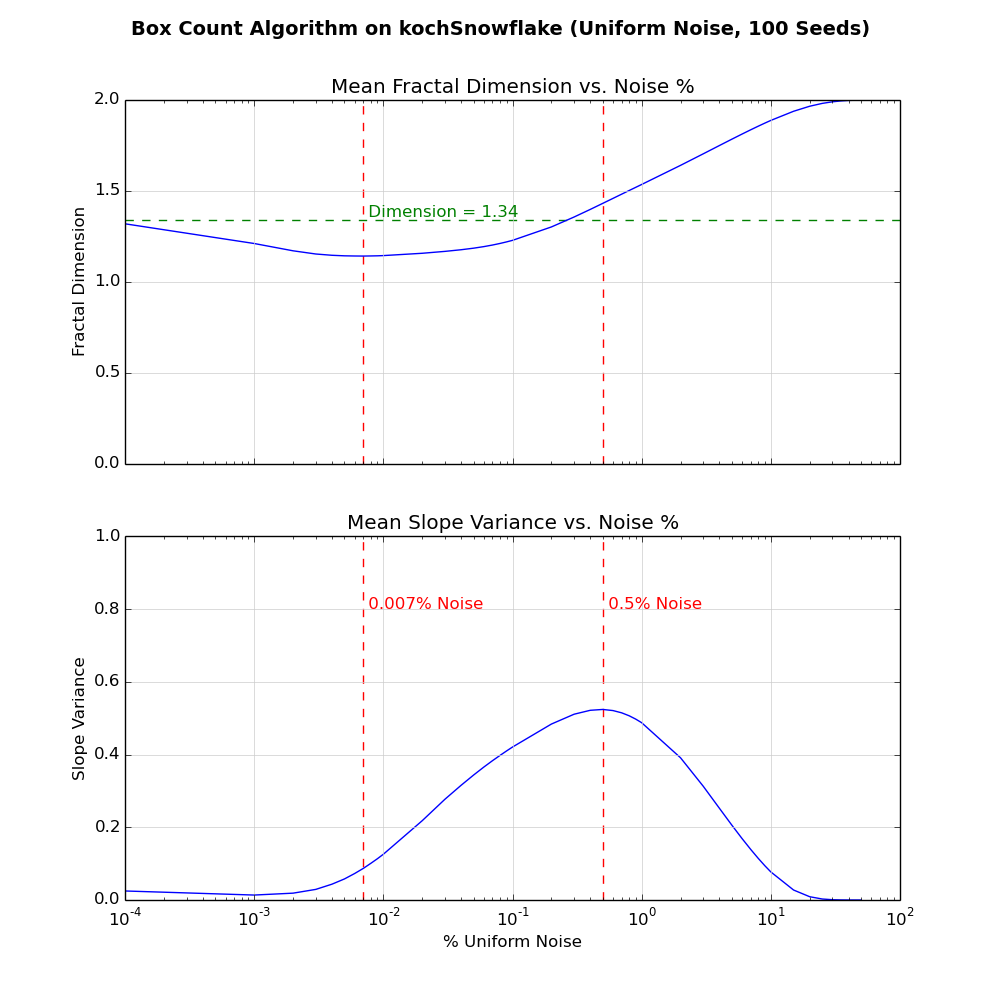
\includegraphics[scale=0.5]{appendixC/Fig_Uniform_DvSV_kochSnowflake.png}}
  \caption[Fractal Dimension and Slope Variance vs. Uniform noise for the  \textit{kochSnowflake.png} image.]{Fractal Dimension and Slope Variance vs. Uniform noise for the \textit{kochSnowflake.png} image.  Results shown are the average of 100 noise seeds.  Highlighted are initial no-noise dimensional estimate, and Uniform Noise percentages where minimum dimension and maximum slope variance occur.}
  \label{fig:kochSnowflake_uniform_result}
\end{figure}

%% PAGE( 36 )
The results of the Box-Counting Algorithm for the uniform noise case on the \textit{kochSnowflake} image are shown in Figure 12.  The top plot shows the change in the mean fractal dimension estimation as the percentage of uniform noise injected into the image increases from 0\% to 50\%.  The mean fractal dimension is calculated by averaging the results of the 100 uniquely seeded uniform noise simulations across the \textit{kochSnowflake} image.  The horizontal dotted line marks the fractal dimension estimation of the \textit{kochSnowflake} image prior to the addition of uniform noise.  At low levels of uniform noise, the fractal dimension estimation initially drops, reaching a minimum value of 1.1416, which occurs at a uniform noise value of 0.007\%.   For a 2100x1800 resolution image, the total number of pixels is 3,780,000, and a 0.007\% uniform noise represents the flipping of only 265 pixels.  After  the 0.007\% noise level, the fractal dimension begins to rise monotonically as the noise level is increased, reaching saturation at a dimensional estimation of 2 as the uniform noise reaches its maximum value of 50\%

\begin{figure}[!b]
  \centering
  \frame{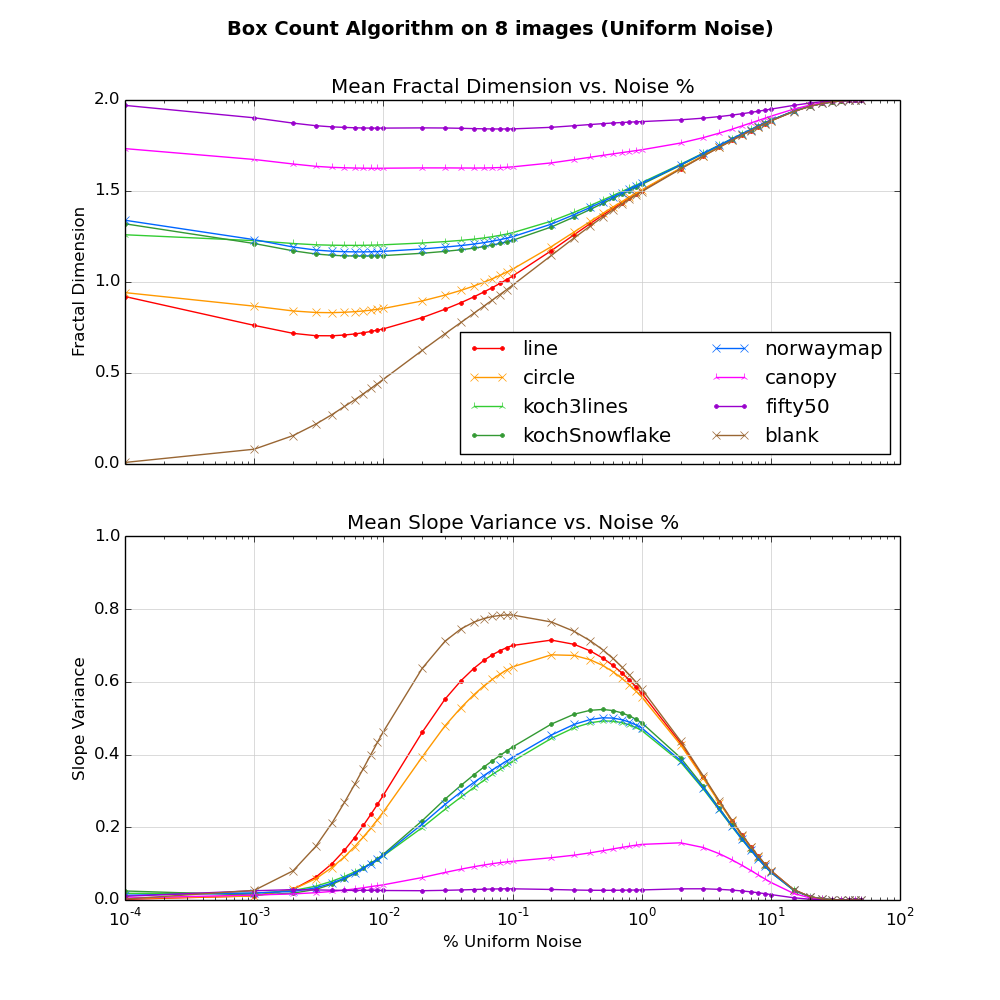
\includegraphics[scale=0.5]{appendixC/Fig_DvsSV_Uniform_Multiplot_blank.png}}
  \caption[Fractal Dimension and Slope Variance vs. Uniform noise for several simulated images.]{Fractal Dimension and Slope Variance vs. Uniform noise for several simulated images.}
  \label{fig:simulated_multi_uniform_result}
\end{figure}

The bottom plot in Figure 12 shows the changes in mean Slope Variance as the uniform noise level increases.  At low and high levels of uniform noise, the value of the slope variance is near zero.  As the uniform noise level increases, the Slope Variance steadily increases until it reaches a peak value of 0.5240 at a 0.5\% uniform noise level, at which point begins to steadily decrease as more uniform noise is added.  Two vertical dashed lines highlight the uniform noise levels where the minimum fractal dimension value and the maximum slope variance level occur.

Several characteristics are present in the dimensional estimate and slope variance curves when plotted against the uniform noise percentage across all images in the test image set.  First, the fractal dimension estimation initially decreases as small levels of uniform noise are injected, eventually reaching some local minimum value.  Once reaching this minimum value, the dimensional estimation then steadily increases as more uniform noise is added, eventually reaching an estimate of 2 as the uniform noise reaches 50\%.  Second, the Slope Variance value increases from its no-noise value as uniform noise is increasing until it reaches a single local maximum value, after which the Slope Variance value drops until reaching 0 as the uniform noise level reaches 50\%.  

%% PAGE( 37 )
Figure \ref{fig:simulated_multi_uniform_result} shows the dimensional estimate and slope variance plots for the full set of simulated images over the uniform noise model.  The top plot shows how the fractal dimension estimation changes as uniform noise is injected into each image, while the bottom plot shows the changes in the slope variance value across the uniform noise range.  Several observations are evident when viewing this data.  The fractal dimension curve for each image shows an initial decrease in value at low levels of uniform noise, though the rate at which each images is affected appears to vary.  The relative rankings of dimension hold very well across the full uniform noise spectrum, with the one exception being the \textit{koch3lines} dimensional estimate swaps places with the \textit{norwaymap} and \textit{kochSnowflake} dimensional curves.  The noise level where the minimum dimensional estimate occurs is directly proportional to initial dimensional estimate, where images with larger initial dimension have a minimum estimate occurring at a larger percentage of uniform noise.

%% PAGE( 38 )
The Slope Variance curves also hold a strong relationship with the initial fractal dimension estimation.  Peak slope variance is inversely proportional to initial fractal dimension, where images with lower initial dimensional estimates produce a higher slope variance peak value.  The uniform noise level at which the peak variance occurs is directly proportional to the initial dimensional estimate as well, where the peak Slope Variance occurs at larger uniform noise levels for images with larger initial dimensional estimates.

A summary of the fractal dimension estimations, minimum fractal dimension noise percentage and maximum slope variance noise percentage results are shown in Table \ref{tab:base_dimensions}.  The strong relative ranking properties are evident across all three of these parameters.

\begin{table}[!b]
    {\hspace{0cm}
    \begin{tabular}{|p{3cm}|c|c|c|}
    \hline & & & \\ [-1.5ex]
    \textbf{Image Name}  & \textbf{No-noise \(D_{m}\)} & \textbf{Minimum \(D_{m}\) Noise \%} & \textbf{Peak SV Noise \%}\\
    \hline & & & \\ [-1.5ex]
    blank         & 0.00 & 0.0\%   & 0.09\% \\
    \hline & & & \\ [-1.5ex]
    circle        & 0.95 & 0.004\% & 0.2\% \\
    \hline & & &  \\ [-1.5ex]
    line          & 0.96 & 0.004\% & 0.2\% \\
    \hline & & &  \\ [-1.5ex]
    koch3line     & 1.26 & 0.006\% & 0.5\% \\
    \hline & & &  \\ [-1.5ex]
    kochSnowflake & 1.34 & 0.007\% & 0.5\% \\
    \hline & & &  \\ [-1.5ex]
    norwaymap     & 1.36 & 0.007\% & 0.5\% \\
    \hline & & &  \\ [-1.5ex]
    canpoy        & 1.74 & 0.009\% & 2.0\% \\
    \hline & & &  \\ [-1.5ex]
    fifty50       & 1.98 & 0.08\%  & 3.0\% \\
    \hline
    \end{tabular}
    }
    \caption{Baseline fractal dimensions for generated test image set, along with uniform noise levels where lowest fractal dimension and peak slope variance occur.}
    \label{tab:base_dimensions}
\end{table}



The \textit{owl} and \textit{fallleaf} natural image sets, which were post-processed using filtering techniques over several threshold values, also exhibit strong relative rankings across the uniform noise spectrum for both the fractal dimension estimations and slope variance calculations, even though their initial fractal dimension estimates vary greatly when using different filtering threshold values.  Figure \ref{fig:leaf_multi_uniform_result} plots the relationships between fractal dimension and slope variance over uniform noise for several different filter thresholds for the \textit{fallleaf} image.  For each threshold case, the same initial dimensional decrease is observed, and the relationship between initial fractal dimension value and minimum dimensional noise location, maximum slope variance value, and maximum slope variance noise location are all preserved. These results are mirrored in the owl image set produced through both edge-detection filtering (Appendix C, Figure \ref{fig:owl-ed_multi_uniform_result}) and threshold filtering (Appendix C, Figure \ref{fig:owl-thresh_multi_uniform_result}).

\begin{figure}[!b]
  \centering
  \frame{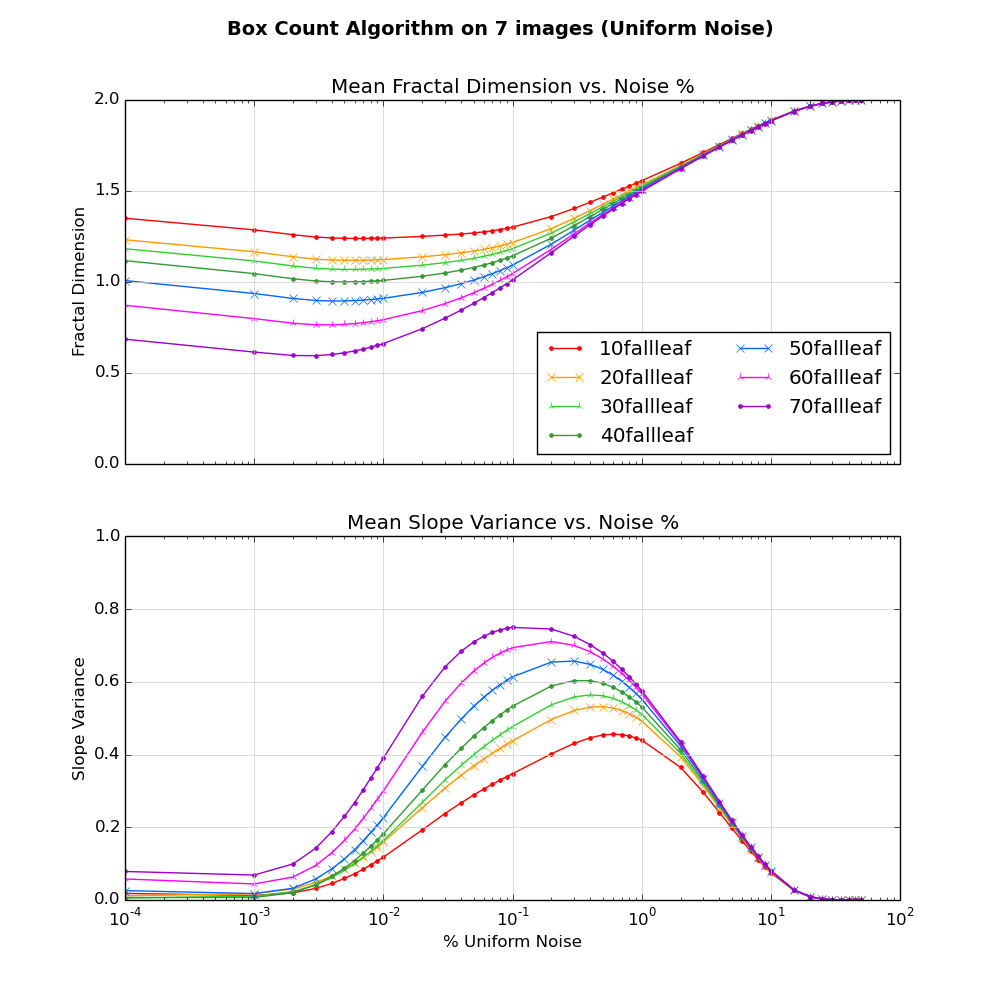
\includegraphics[scale=0.5]{appendixC/Fig_DvsSV_Uniform_Multiplot_70fallleaf.png}}
  \caption[Fractal Dimension and Slope Variance vs. Uniform noise for several edge-detection filtered thresholds for the fallleaf image.]{Fractal Dimension and Slope Variance vs. Uniform noise for several edge-detection filtered thresholds for the fallleaf image.}
  \label{fig:leaf_multi_uniform_result}
\end{figure}


% -------------------------------------------
% 
%     Results : Gaussian Noise
%
% -------------------------------------------
\section{\underline{Gaussian Noise Results}}
%% PAGE( 39 )
Analysis of the Box-Counting Algorithm dimensional estimates as Gaussian noise is injected into the image offers a different set of results from the uniform noise model.  Where the uniform noise model has the potential to affect any pixel within the image space with equal probability, the effects of Gaussian noise are concentrated in the areas of an image where signal is present, resulting in noise profiles which are tied to the actual image content.  A second major difference between the uniform and Gaussian noise models involves how a completely obfuscated image appears in each case.  The uniform noise model at 50\% noise produces an image where roughly half the pixels are black.  In the Gaussian noise case, a completely obfuscated image contains roughly the amount of black pixels that were present in the initial image.  An image of a line containing a small number of black pixels would result in a final noisy image containing the original number of black pixels uniformly distributed in the image space.  These differences play a role in the following results.  The full set of Gaussian noise plots across the test image set can be found in Appendix D

Figure \ref{fig:kochSnowflake_gaussian_result} shows the plot of the dimensional estimate and slope variance curves versus increasing levels of Gaussian noise for the \textit{kochSnowflake} image.  The top plot illustrates how the fractal dimension estimation changes as sigma is increased from 0 to 1000.  At low sigma levels, the dimensional estimate increases until reaching a sigma level of 10, before entering a period of alternating periods of decreasing and increasing estimate levels.  The corresponding slope variance curve, plotted below, shows a slope variance value which rises as the sigma level is increased, until reaching its peak value at the largest simulated sigma level of 1000.  In the Gaussian noise case, a local slope variance maximum does not exist.  

\begin{figure}[!b]
  \centering
  \frame{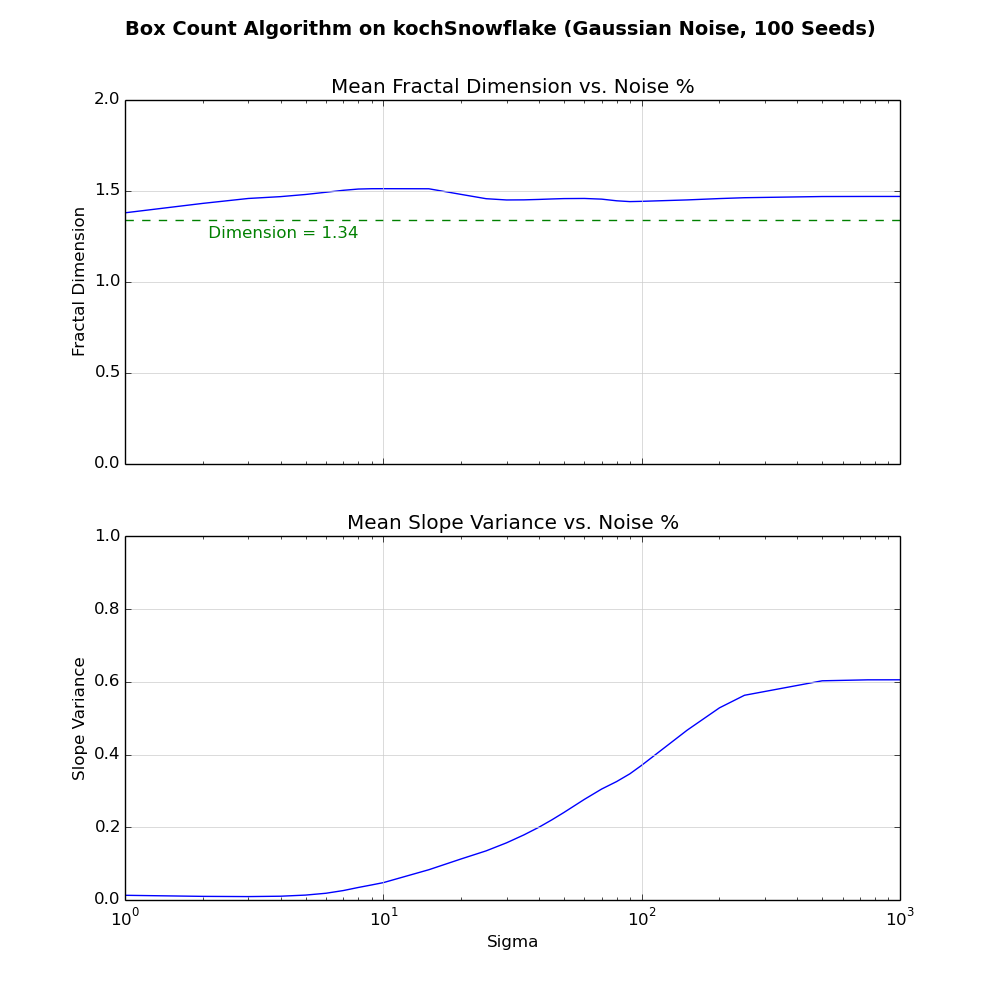
\includegraphics[scale=0.5]{appendixD/Fig_Gaussian_DvSV_kochSnowflake.png}}
  \caption[\(D_{m}\) and Slope Variance versus Gaussian noise for kochSnowflake.png]{\(D_{m}\) and Slope Variance versus Gaussian noise for kochSnowflake.png.  Results shown are the average of 100 noise seeds.}
  \label{fig:kochSnowflake_gaussian_result}
\end{figure}

%% PAGE( 41 ) / %% PAGE( 42 )
The fractal dimension estimation and slope variance curves for the simulated image set is shown in Figure \ref{fig:simulated_gaussian_multi_result}.  The top plot shows the changes in fractal dimension as the sigma value for injected Gaussian noise is increased from 0 to 1000.  The dimensional estimate curves in the Gaussian noise case do not exhibit a common profile as is seen under the uniform noise model.  For the \textit{fifty50} image, there is an increase in dimensionality, followed by a irregular drop in dimensionality, whereas the \textit{canopy} image exhibits a steady climb in dimensionality throughout the Gaussian noise range.  The \textit{koch3lines}, \textit{kochSnowflake}, and \textit{norwaymap} image all have similar initial dimensional estimates, and while a gradual increase in dimensional estimation occurs as sigma is increased, the relative dimensional rankings of these three images switch several times at various sigma levels.  The \textit{line} and \textit{circle} image also have initial dimensional estimates which are very close, yet the dimensional estimate of the  \textit{line} image at maximum Gaussian noise is lower than the initial estimate, while the \textit{circle} image shows a higher final dimensional estimate.  Unlike the uniform noise model where the noise percentage location of the minimum dimensional estimate was directly proportional to the initial dimensional estimate, in the Gaussian noise case a relationship between peak dimensional estimate location and the initial fractal dimension estimation does not appear to exist, with a peak sigma value for the low-dimensional \textit{circle} image occurring between the peak sigma values for the higher dimensional \textit{kochSnowflake} and \textit{norwaymap} images.

\begin{figure}[!b]
  \centering
  \frame{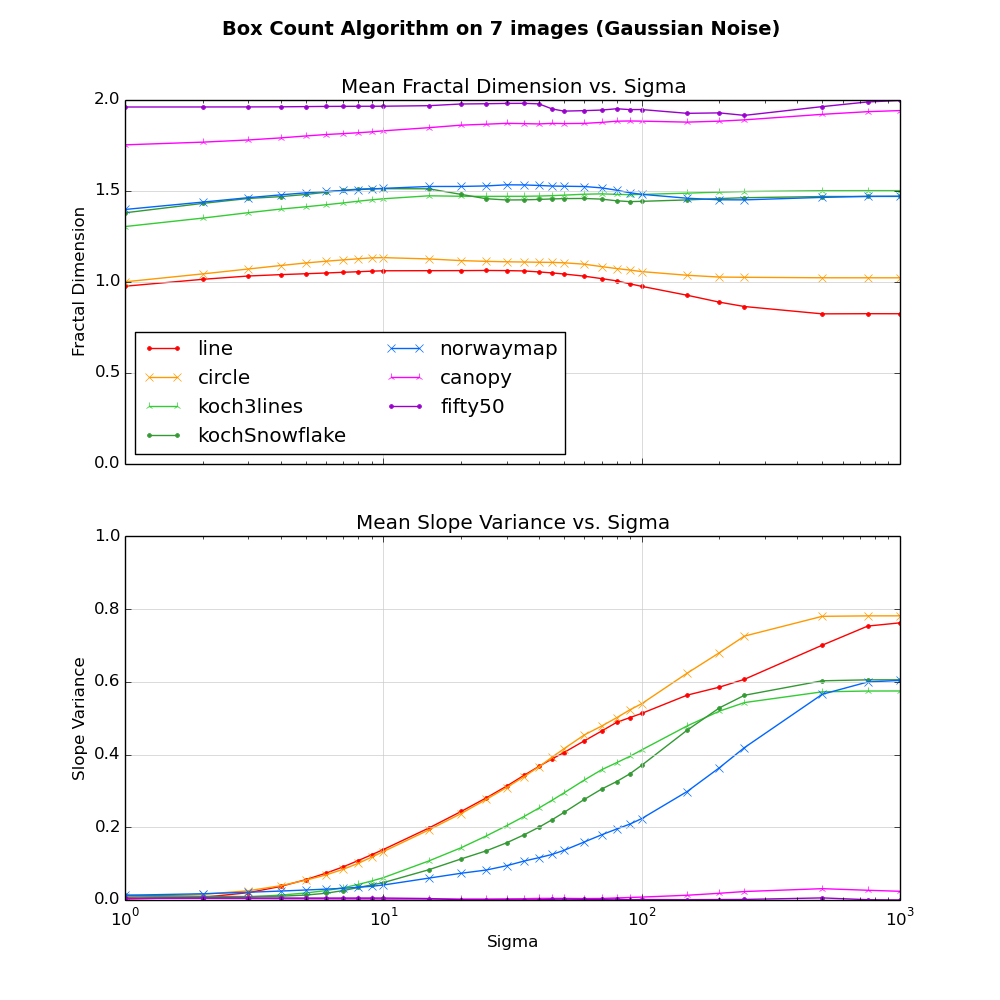
\includegraphics[scale=0.5]{appendixD/Fig_DvsSV_Gaussian_Multiplot_fifty50.png}}
  \caption[\(D_{m}\) and Slope Variance versus Gaussian noise for the simulated image set.]{\(D_{m}\) and Slope Variance versus Gaussian noise for the simulated image set.  Results shown are the average of 100 noise seeds.}
  \label{fig:simulated_gaussian_multi_result}
\end{figure}

The bottom plot in Figure \ref{fig:simulated_gaussian_multi_result} shows the change in slope variance as sigma is increased.  The relationship between the simulated images' slope variance curves also do not show a strong relationship with respect to initial fractal dimensional estimates.  The slope variance value increases as Gaussian sigma increases across the simulated image set, although the rate of increase differs from image to image, with the slope variance curves for the \textit{line} and \textit{kochSnowflake} image showing multiple inflection points.

Inconsistent relationships between the dimensional and slope variance curves are present in the leaf image edge-detection filtered set as well.  While a relative ranking between the dimensional estimate curves exists between the entire filtered threshold range, the images with higher initial fractal dimension estimates tended to rise throughout the Gaussian noise sigma range, where lower dimensional images showed an initial dimensional estimate rise, then dropped as the sigma value reached its maximum value.  In the slope variance curves for higher dimensional images, the slope variance curve's maximum value was inversely proportional to the initial dimensional estimate, but this relationship breaks down at lower dimensional images (see Appendix D, Figure \ref{fig:fallleaf_gaussian_multi_result}).



% =====================================================================
% 
%      D I S C U S S I O N
%
% =====================================================================
\chapter{\textbf{DISCUSSION}}
%% PAGE( 44 )
First, the selection of a Box-Counting Algorithm secondary key metric is explored and the reasoning behind the choice of slope variance as the key of choice is discussed.  Next, the relationship between the dimensional estimate and the slope variance in the uniform noise case is explored.  Three distinct regions are defined which determine whether a dimensional estimate can be considered valid, and it is shown that a hierarchical relative ranking between dimensional estimates across the image set exist within these regions.  Next, the dimensional and slope variance relationship as an image is influenced by Gaussian noise is presented, and the limitations of this noise model are discussed.  Finally, a list of considerations is presented which outline steps to ensure the validity of a dimensional estimation obtained by the BCA.

\section{\underline{Secondary Key Selection}}
Four measures of linearity were chosen as candidates for a secondary key which would pair with the dimensional estimate to strengthen the estimate value.  These keys were the slope variance, the population slope variance, the sum of the differences, and the sum of the central differences.  These keys were tested in simulations using the uniform noise model.  Of these four keys, only the variance calculations produced a data set which identified distinct regions when paired with the dimensional estimation data set, and these regions were evident in all simulations across the entire test image set.

The slope variance used the statistical calculation for unbiased variance, and therefore produced values that were slightly higher than the unbiased slope population variance results.  Otherwise, the two behaved identically in the uniform case.  The profile of the slope variance curve on the simulated image set presented a data set containing a single local maximum point, and the location on the noise axis for this maximum was directly proportional to the initial dimensional estimate.  The magnitude of the maximum slope variance was inversely proportional to the initial dimensional estimate.  

%% PAGE( 45 )
The sum of the differences and sum of the central differences curves produced results that were difficult to associate with the fractal dimension estimation curves.  Many images produced data curves which contained several local maximum and minimum values.  Due to the irregularity of the result of these metrics, and due to the strength of the slope variance data set, the slope variance was chosen to be the secondary key used in this research.

While the slope variance offers a useful comparison curve under the uniform noise model, it was not as helpful under the Gaussian noise model.  Under a uniform noise model, each image was eventually completely obfuscated once the uniform noise reached 50\%.  In the Gaussian noise case, where signal is diffused, the end result was a spreading of the signal across the image area, where the density of black pixels was inversely proportional to the initial number of black pixels in the image.  The rate of this diffusion is related to the shape of the geometry, so images containing similarly dimensional geometries might diffuse at different rates, which can change relative dimensional rankings between images as the level of Gaussian noise increases.

\section{\underline{Uniform Noise Simulations}}
Under the presence of uniform noise, the following three regions are identified. The first region is defined where uniform noise is initially introduced into an image, resulting in a drop in the dimensional estimation and a rise in the slope variance calculation.  The second region is defined where the dimensional estimate begins to increase along with the continued increase in slope variance.  The third region is defined after the slope variance has reached its peak value, and the slope variance drops while the dimensional estimate increases to a maximum value of 2.

%% PAGE( 46 )
In the first region, where low noise conditions exist, there is initially a drop in the fractal dimension estimation.  This can be explained by viewing the sparse noise pixels as the inclusion of low-dimensional point data.  These points lower the overall dimensional estimate of the global image space due to the space now containing a mixture of high and low dimensional geometries.  The effect of mixing dimensional geometries is also observed in the \(koch3lines\) results (Appendix C, Figure \ref{fig:koch3lines_uniform_result}), where the inclusion of 3 lines (lower dimensional signals) over the Koch Snowflake (a higher dimensional signal) results in an overall lower fractal dimension estimation for the image.  The increase in slope variance is caused due to the mixing of dimensional signals affecting how the dimension of the image appears at different scales.  In other words, the apparent dimension of the geometry begins to shift as the box size is changed from small to large, causing disagreement between point-pair slope estimates.

In the second region, once the number of additive noise pixels increases to a sufficient amount, they begin to appear less as low-dimensional points and more as a higher dimensional space filling geometry.  As uniform noise fills empty regions in the image, the dimensional estimate now begins to rise, and continues to rise until the uniform noise reaches 50\%.  In the second region, the slope variance is also rising due to the stronger conflict in which geometry is the dominant dimensional force: noise or the original image.  At the peak slope variance uniform noise percentage, both the uniform noise and the original image content are at peak contention.

The third region, the uniform noise is now the dominant dimensional force, overwhelming the original image content.  The fractal dimension estimation increases monotonically to a final value of 2 as the uniform noise continues to evenly fill all empty spaces, and as this fill is evident at all levels of scale, the slope variance begins to decrease as the noise percentage is increased.  Because noise is the controlling geometry in the third region, the fractal dimension of the original image content must be considered lost, and a classification of an image using the fractal dimension taken in the third region must be considered a poor classification.  Classifications made in the first two regions can still be considered valid, although an understanding of which region an estimate occurs is vital in order to make relative ranking conclusions.

%% PAGE( 47 )
\section{\underline{Gaussian Noise Simulations}}
The identification of regions where relative ranking estimates are valid across Gaussian noise simulations is more difficult than the uniform noise case.  

This is due to the relationship between the signal geometry and the Gaussian filter itself.  Images containing signals with similar dimensional content yet differing geometries will be affected in dissimilar ways as the Gaussian noise takes hold.  Gaussian noise attacks small signals first, blurring and destroying the roughness of small signals and making them appear as higher dimensional.  In the extreme case, a Gaussian noise with a large sigma will spread any countable pixels within an image into a uniform cloud, resulting in an ultimate noise case mirroring pure uniform noise at a certain pixel level.  The geometry of the underlying image, however, determines the path the dimensionality estimate will take in reaching this saturation point.

For example, an image containing a single straight line would require a very large sigma to spread the line pixels uniformly across the image boundaries.  An image containing a circle, while dimensionally similar to a line, already contains pixels which are more evenly spread out across the image.  The diffusion of these pixels would not happen at the same rate as that of the line.  

Figure \ref{fig:swapping_gaussian_multi_result} shows the dimensional estimation and slope variance curves for the \textit{15fallleaf} and \textit{kochSnowflake} image over the influence of Gaussian noise.  In the no-noise case, the Koch Snowflake is shown to have a higher fractal dimension than the leaf image filtered using an edge-detection filter at a threshold of 15.  As Gaussian noise is increased, however, the relative rankings of these images' dimensional estimates switch.  The \textit{15fallleaf} image originally contains 49323 black pixels, while the \textit{kochSnowflake} image contains 32950 black pixels.  While the Koch Snowflake geometry has greater complexity in the no-noise case than that of the \textit{15fallleaf} image, and therefore has a higher fractal dimension, eventually the rankings are controlled by the density of black pixels present in the original image.

\begin{figure}[!b]
  \centering
  \frame{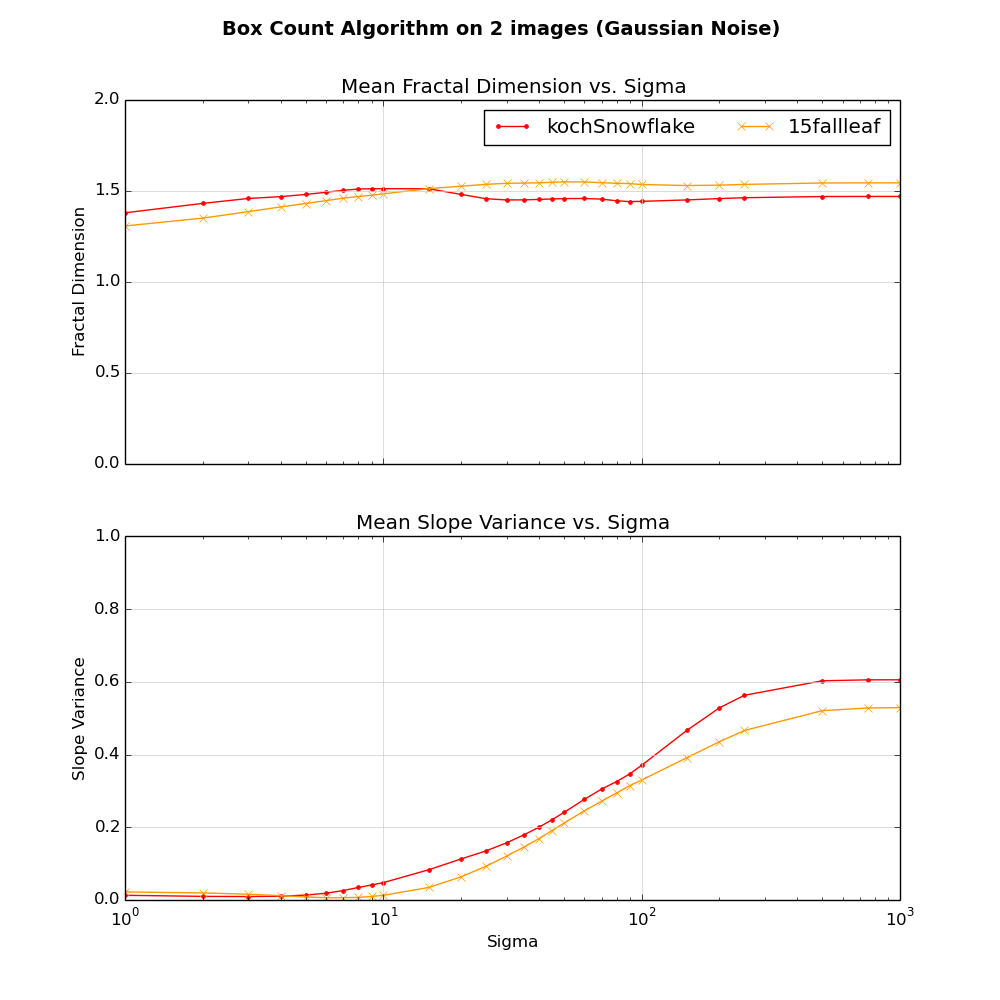
\includegraphics[scale=0.5]{appendixD/Fig_DvsSV_Gaussian_Multiplot_15fallleaf.png}}
  \caption{The relative ranking between the kochSnowflake image and the 15fallleaf image are changed in the presence of moderate Gaussian noise.}
  \label{fig:swapping_gaussian_multi_result}
\end{figure}

%% PAGE( 48 )
The Gaussian Noise case also offers difficulties while using the slope variance as a secondary key.  In the Gaussian Noise case, the three unique regions present under the uniform noise model do not exist, so it is difficult to tell if or when we have reached a particular level of noise.  The slope variance has no peak value, and preserving relative rankings based on slope variance information is difficult, if not impossible.  This means that relative rankings using fractal dimension estimates might be weakened, and perhaps even destroyed in the presence of moderate Gaussian Noise.


% ===========================
%
%    C O N C L U S I O N S
%
% ===========================
%% PAGE( 49 )
\section{\underline{Conclusions}}
It has been shown in previous research that there are many properties of digital images that distort the fractal dimension estimate for an image, such as line thickness, image post-processing filtering, noise, and non-uniform scaling effects.  The question asked is "Can relative comparisons between digital images be meaningful based on the fractal dimension estimations using the Box-Counting Algorithm calculation in spite of all these inaccuracies?"

After analyzing several secondary key measures calculated over the iterations of the BCA, the slope variance proved to provide an interesting relationship with the fractal dimension estimate in the uniform noise case across the entire set of test images.  Slope variance is easy to calculate and its computation ties naturally into the iterative nature of the BCA.

Under the influence of uniform noise, the relationship between the fractal dimension estimation and slope variance curves revealed three distinct regions of dimensional estimate behavior.  These regions are defined by the location of the minimum fractal dimension estimate and the location of the maximum slope variance. 

The first region is characterized by fractal dimension decreasing and slope variance increasing at very low levels of uniform noise.  In this region noise plays the roll of lowering the dimension of the global image space as low-dimensional pixels are added.  The second region is characterized by fractal dimension increasing along with increasing slope variance.  In the second region, noise is beginning to fill space, increasing the dimensionality of the global image space, although the original image geometry is still the dominant force influencing the dimensional estimate.  The third region is characterized by an increase in fractal dimension and a decrease in slope variance.  In the third region, the noise has become the controlling geometry in the image, and while the relative ranking of the estimates among similarly treated images is preserved, dimensional information about the original image geometry is now unrecoverable for the purpose of classification.

%% PAGE( 50 )
Across all images tested, the relative rankings of dimensional estimates across images is strongly preserved in the presence of uniform noise.  However, even small amounts of uniform noise can greatly affect the dimensional estimate.  In Figure \ref{fig:threelines} the drastic effect of a small amount of uniform noise is shown.  In this case, the line image was pre-injected with uniform noise so that a fractal dimension estimate occurred in each of the three regions.  The \textit{P0.003line} image was created by injecting 0.003\% uniform noise into the image, which is the uniform noise value in which the minimum fractal dimension occurs, and then running the noisy image through the BCA process.  The \textit{P0.3line} image was injected by 0.3\% uniform noise, which is a noise level which pushes the estimate into the third region, and then run through the BCA process.  The results of the fractal dimension estimations and slope variance of these two noisy line images was then compared to the original line image.

\begin{figure}[!b]
  \centering
  \frame{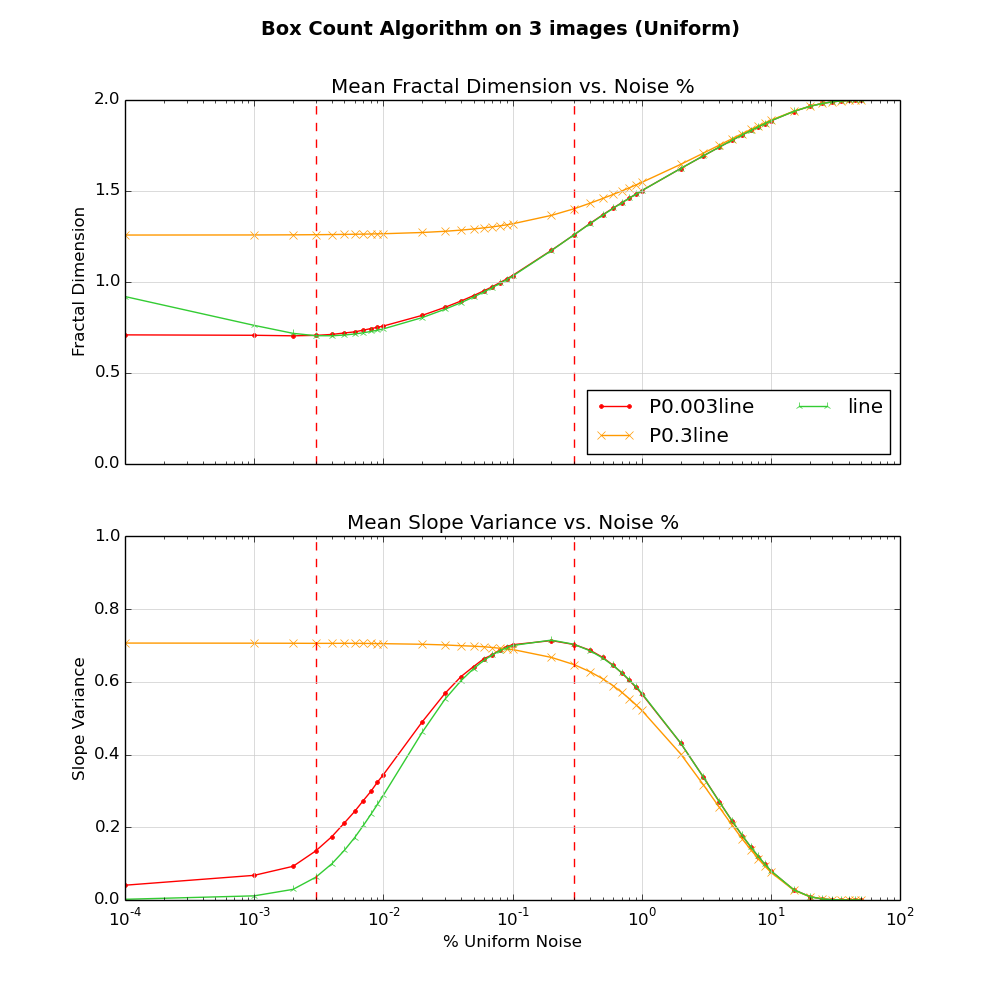
\includegraphics[scale=0.5]{figures/Figure_DvsSV_Uniform_BIGline.png}}
  \caption[The \(D_{m}\) and slope variance curves are plotted for three line images, each initially injected by a small amount of uniform noise.]{The \(D_{m}\) and slope variance curves are plotted for three line images, each initially injected by a small amount of uniform noise.  The line image had no initial noise added, P0.003line had 0.003\% uniform noise added, and P0.3line had 0.3\% uniform noise added. }
  \label{fig:threelines}
\end{figure}

From the plots of the three line cases in Figure \ref{fig:threelines} the following key points can be made.  First, even though the image contained the same geometric figure (a line), the BCA produced initial fractal dimension estimations which varied greatly.  Second, for the line image case, it is shown that the dimensional estimate initially drops when a small amount of uniform noise is added, indicating that the dimensional estimate is produced in the first region.  For the \textit{P0.003line} image case, the dimensional estimate increases as small levels of uniform noise are added, while the slope variance also increases.  In this case we are in the second region, and are able to continue to add uniform noise until the peak slope variance is found.  For the \textit{P0.3line} case, as small levels of uniform noise are added, the dimensional estimate increases and the slope variance decreases.  In this case we are in the third region, and it becomes difficult, if not possible, to determine how far back the slope variance peak might have occurred.

While the \textit{P0.003line} case initial dimensional estimate differs greatly from the original \textit{line} dimensional estimate, the peak slope variance values are the same in both cases.  This key potentially allows for the correction of the \textit{P0.003line} dimensional estimate to be closer with the actual dimension of the original image geometry.

%% PAGE( 51 )
For the Gaussian noise model, this type of correction is not possible due for two reasons.  First, due to the nature of Gaussian Noise, the image geometry strongly influences the effect of Gaussian noise at differing sigma values.  Therefore two similarly dimensional geometries will be affected by Gaussian noise at differing rates depending on how these geometries are folded in the two dimensional space.  Second, because Gaussian noise only moves pixels around, at high sigmas the dimension and slope variance eventually settles to a final value mirroring the blank image uniform noise case at a particular signal level.  This means there is not a stable set of regions defined by slope variance in this case, and it is difficult (or perhaps not possible) to determine in the Gaussian noise case where an estimate lies in the curve.  This means it would be very difficult (or perhaps not possible) to correct an estimate for a stronger relative ranking using fractal dimension.

Finally, there appears to be a strong linear relationship between the peak slope variance in the uniform noise case and the initial no-noise fractal dimension estimation.  Plotting the fractal dimension versus the peak slope variance for a large subset of the image test set highlights this relationship (Figure \ref{fig:finalresult}).  This linear relationship provides an interesting lead for future work and might provide a "best-guess" estimate for predicting the no-noise fractal dimension for dimensions found to exist in the first two regions.  Also, this linear relationship could imply that a fractal dimension estimate found in the third region would now provide an upper bound on the no-noise dimensional estimate for an image.

\begin{figure}[!b]
  \centering
  \frame{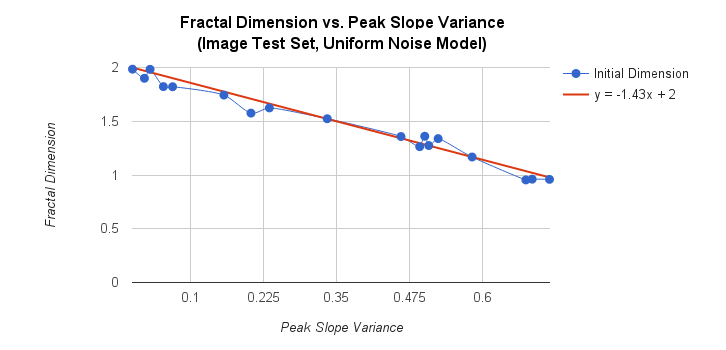
\includegraphics[width=\textwidth]{figures/finalResult.png}}
  \caption[The linear relationship between the fractal dimension and the peak slope variance under the uniform noise model]{The linear relationship between the fractal dimension and the peak slope variance under the uniform noise model across the test image set with an \(R^{2}\) value of 0.967.}
  \label{fig:finalresult}
\end{figure}

In conclusion, it appears that while image processing and noise greatly affect the accuracy of a fractal dimensional calculation, in applications where relative ranking comparisons are based upon fractal dimension calculations, this ranking may be preserved, assuming steps are insured to standardize the image post-processing steps, a uniform noise model, and an understanding of which regime a dimensional estimate exists.


\section{\underline{Future Study}}
There are several areas in which the work in this study could be extended, a few of which are listed here.  The search for a secondary key was not exhaustive, and metrics such as the R-squared value of a curve fit of the fractal dimension slope line could be explored as providing a relationship with the fractal dimension estimate.  A key point of this study was to show that such secondary key relationships do exist that may strengthen the classification properties of fractal dimension for digital images.

It was shown through empirical study on known geometries how rank relative estimates hold true over a wide range of uniform noise conditions, but further testing could expand the test image set, providing examples of more known fractal geometries as well as natural examples, such as a wider selection of leaf samples, or more complex images such as cancer cells or MRI files.  A classification of leaves, for example, could test whether the addition of uniform noise could strengthen the ranking and prediction of leaf types.

Also, this study was limited to studying the effect of only two noise models, uniform and Gaussian, on fractal dimension estimates from digital images.  These models only offer a sample of the types of noise that may be injected into a digital image.  Other studies have measured the effects of influences such as edge thickness, image resolution and scaling effects, and signal placement within an image.  These studies could be extended to map the effects of these properties on the slope variance or another secondary key in order to determine if valuable information might exist.




% =====================================================================
%
%      IMAGE SOURCES - not sure how to credit...
%
% =====================================================================
% Fig: fractal - modified from: 
% https://commons.wikimedia.org/wiki/File:Sierpinski8.svg
% http://www.wimp.com/animalcamo/ -- thesis image source for owl image

\newpage





% Multi-line comment to remove formatting from report...but to retain example information
\begin{comment}

% end of multi-line comment
\end{comment}

% -- Does not currently render correctly.
%\subsubsection{Tertiary Section Headings} 
%If you need a tertiary section heading, then follow the rules for primary section headings except they should be in italics and do not underline.

% - NOTE: changing myplain to ieeetr to order by usage instead of alphabetized. -mcm
\bibliographystyle{ieeetr}
\clearpage
\markboth{}{}
\addcontentsline{toc}{chapter}{BIBLIOGRAPHY}
\bibliography{references}


% Appendices formatting is not yet correct --mcm
% Formatting by hand -- hopefully we can get this close
\clearpage
% ==============================================================
%
% TITLE PAGE FOR APPENDICIES
%
% ==============================================================

\begin{center}
\vspace*{\fill}
\addcontentsline{toc}{chapter}{APPENDICES}
\textbf{APPENDICES}
\vspace{60mm}  % use this amount to center the 'APPENDICES' title

\textcolor{white}{ Spacing to Move Appendices title up}
\vspace*{\fill}
\end{center}

\clearpage

\addcontentsline{toc}{chapter}{APPENDIX A - SOURCE CODE}
\begin{center}
\textbf{APPENDIX A}

\textbf{SOURCE CODE}
\end{center}
The entire code base can be found at \url{https://github.com/mcm7f/thesis/}.  The key files are \textit{bca.py}, which performs the BCA on an post-processed image over the uniform and/or Gaussian noise range, and \textit{aggregator.py}, which takes a set of log files generated from the BCA and computes the average dimension, slope variance, and standard errors of the data set.  The plots used in this document were generated using the \textit{figure\_creator.py} program.



\clearpage

% ================================================================
%
%  A P P E N D I X   B  - Test Images
% 
% ================================================================
\addcontentsline{toc}{chapter}{APPENDIX B - TEST IMAGES}
\begin{center}
\textbf{APPENDIX B}

\textbf{TEST IMAGES}
\end{center}

Not included is a 2100x1800 pixel blank.png image consisting of nothing but white pixels.

%Fig 20
\begin{figure}[!b]
  \centering
  \frame{
\includegraphics[width=\textwidth]{appendixB/line.png}}
  \caption[2100x1800 pixel line]{2100x1800 pixel line, 1 pixel width}
  \label{fig:line_png}
\end{figure}

\begin{figure}[!b]
  \centering
  \frame{
\includegraphics[width=\textwidth]{appendixB/circle.png}}
  \caption[2100x1800 pixel circle]{2100x1800 pixel circle, 1 pixel width}
  \label{fig:circle_png}
\end{figure}

\begin{figure}[!b]
  \centering
  \frame{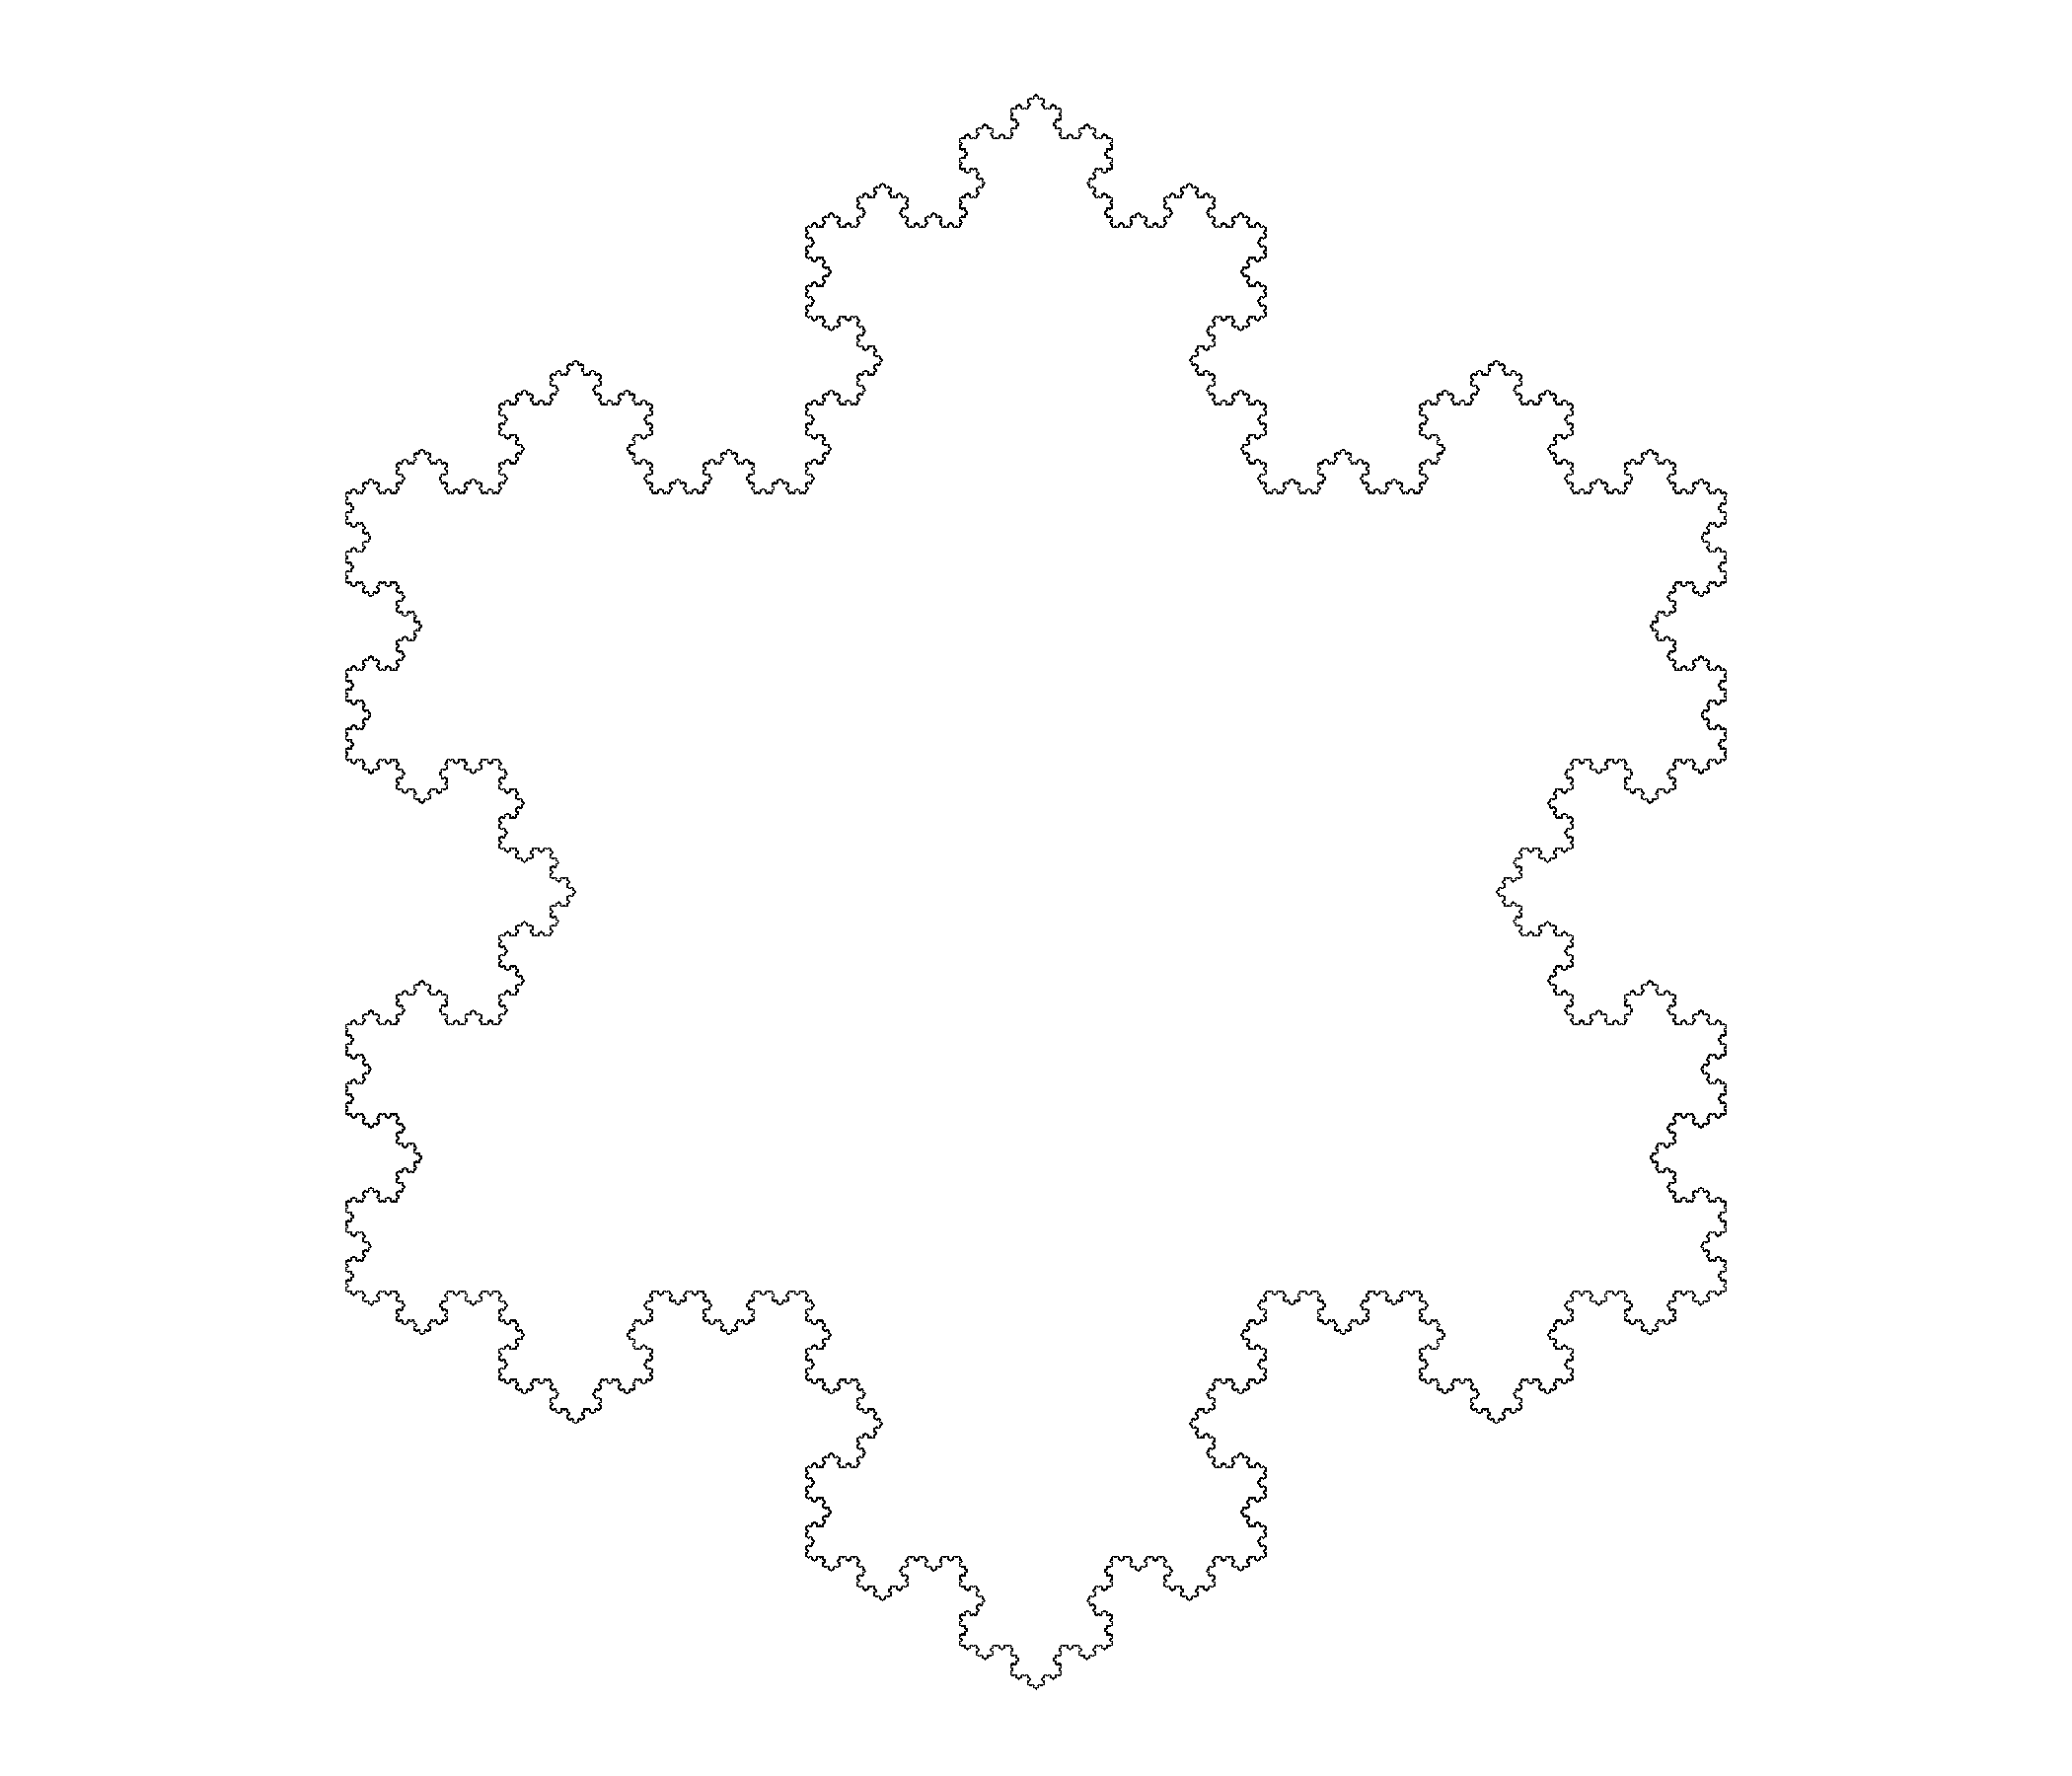
\includegraphics[width=\textwidth]{appendixB/kochSnowflake.png}}
  \caption[2100x1800 pixel kochSnowflake]{2100x1800 pixel kochSnowflake, derived from \url{https://upload.wikimedia.org/wikipedia/commons/e/e9/Koch_Snowflake_7th_iteration.svg}}
  \label{fig:kochSnowflake_png}
\end{figure}

\begin{figure}[!b]
  \centering
  \frame{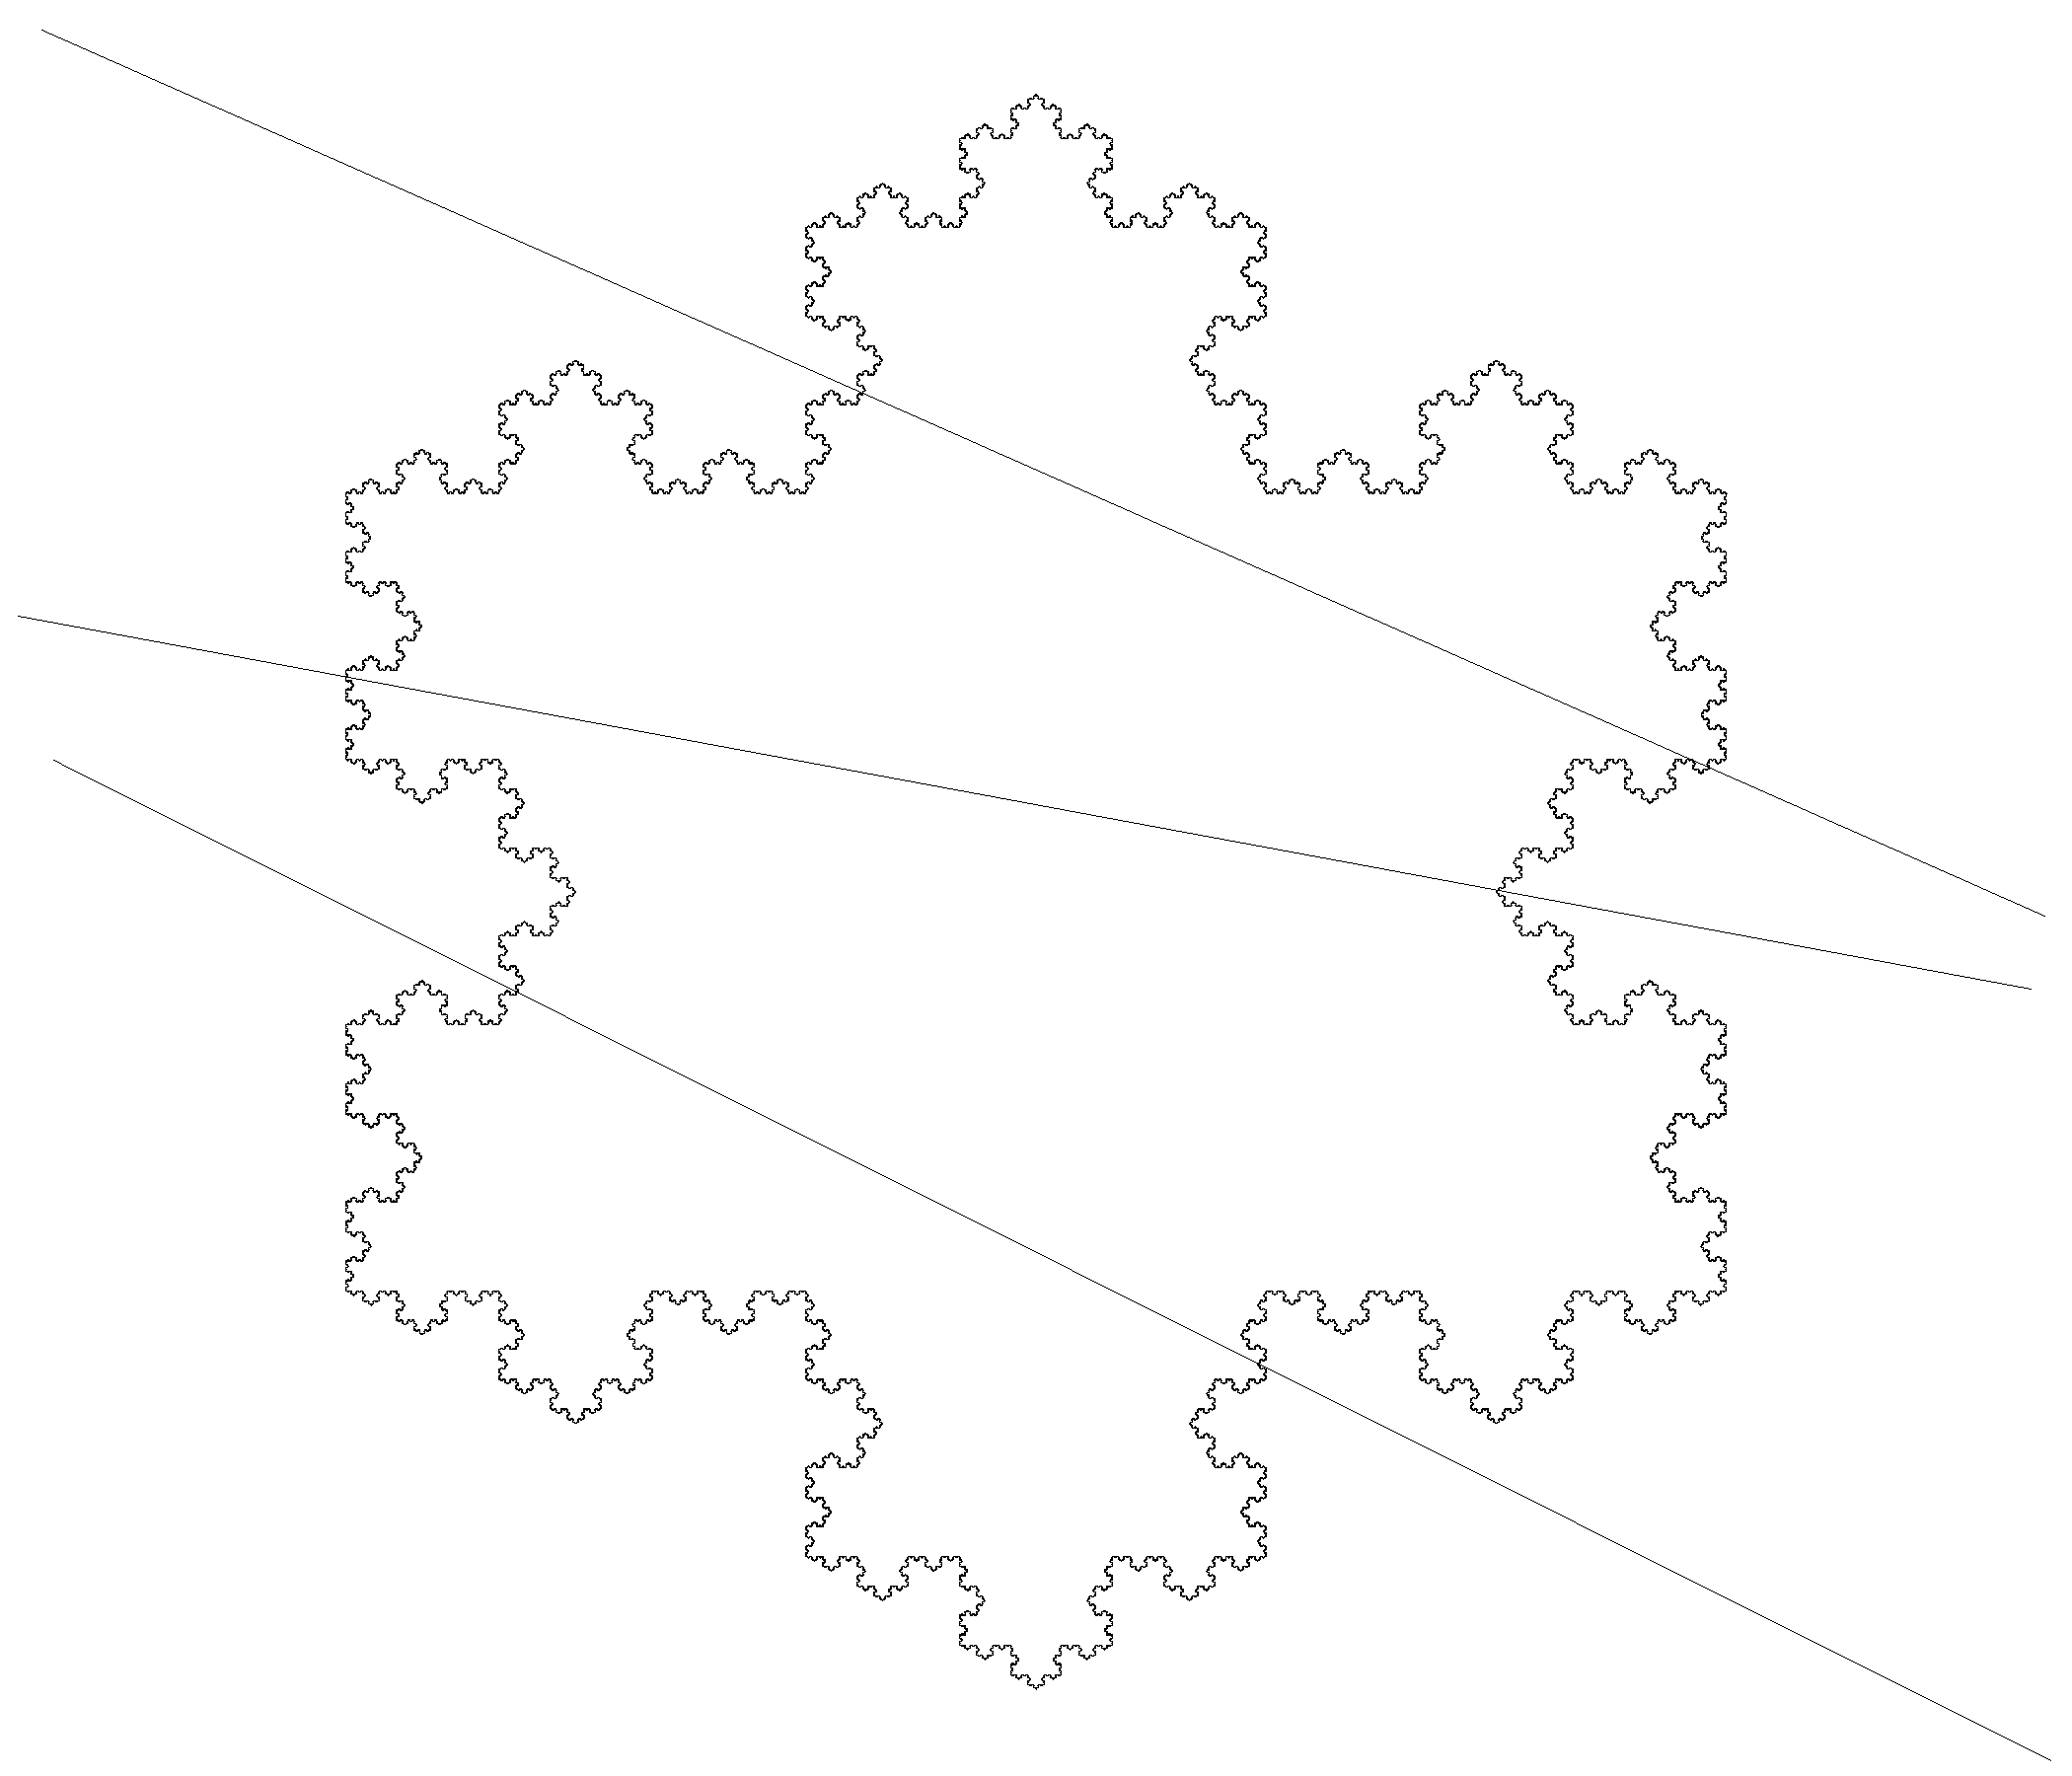
\includegraphics[width=\textwidth]{appendixB/koch3lines.png}}
  \caption[2100x1800 pixel koch3lines]{2100x1800 pixel koch3lines}
  \label{fig:koch3lines_png}
\end{figure}

\begin{figure}[!b]
  \centering
  \frame{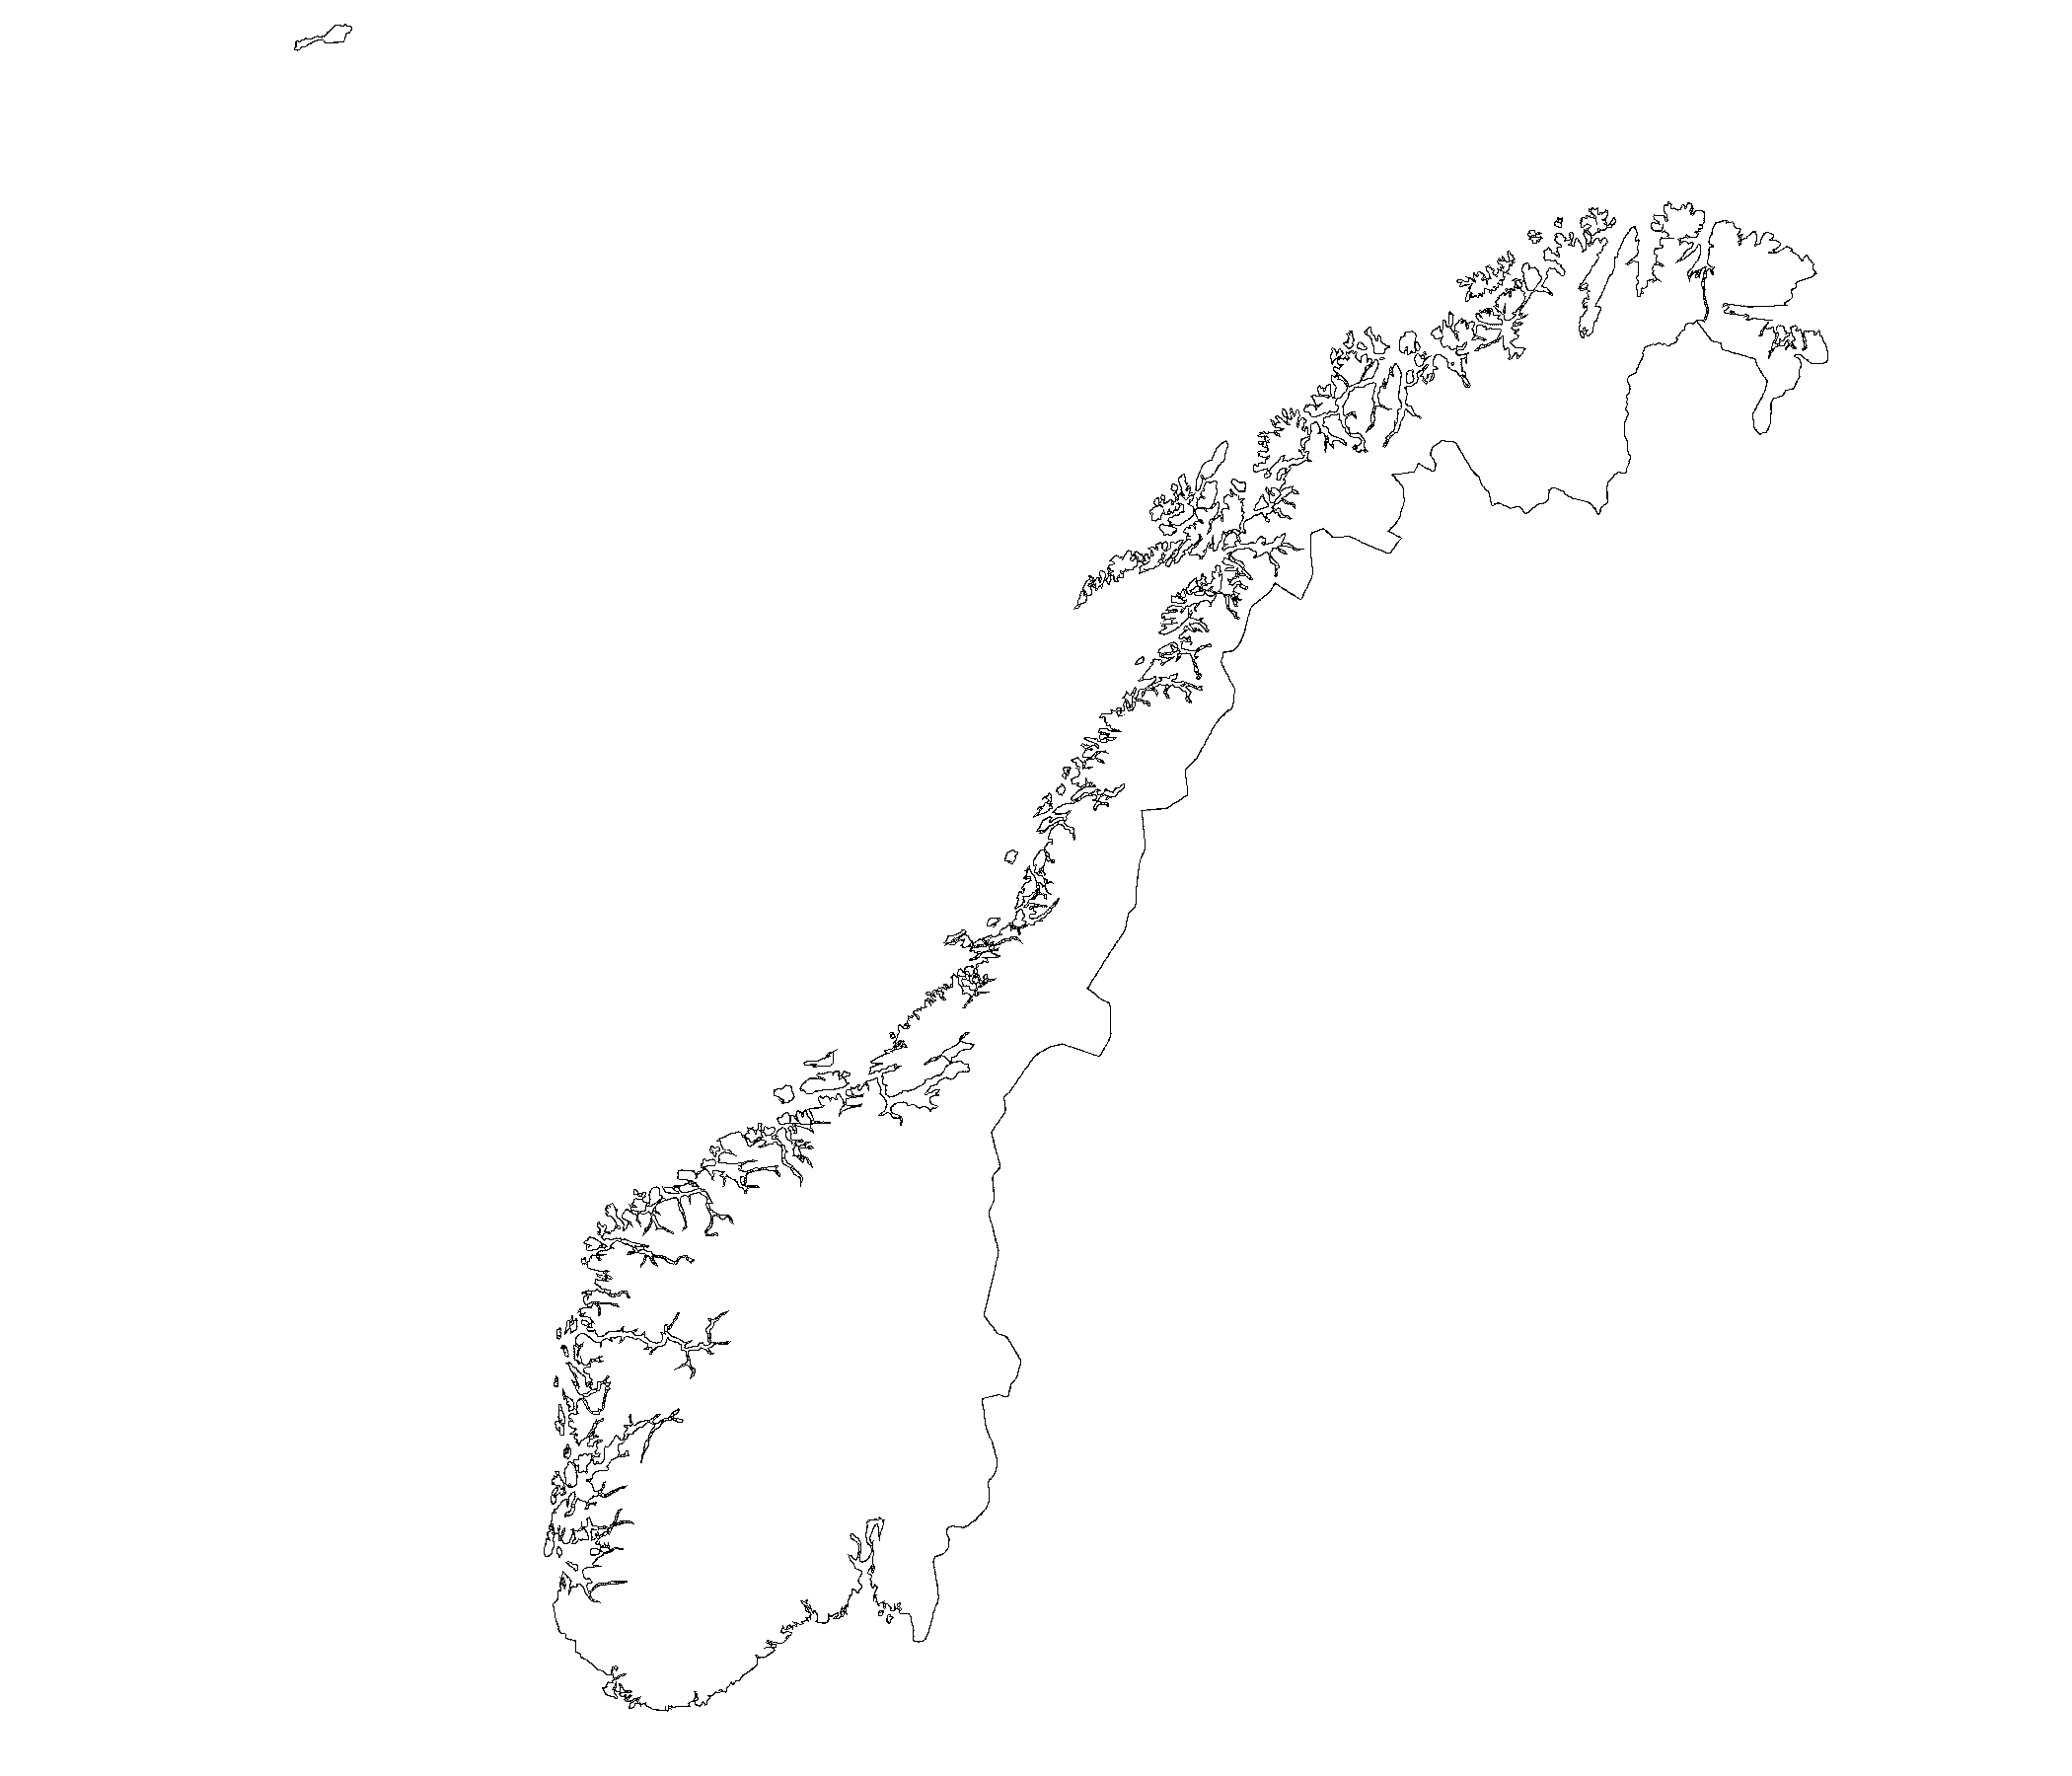
\includegraphics[width=\textwidth]{appendixB/norwaymap.png}}
  \caption[2100x1800 pixel map of norway]{2100x1800 pixel map of norway}
  \label{fig:norwaymap_png}
\end{figure}

\begin{figure}[!b]
  \centering
  \frame{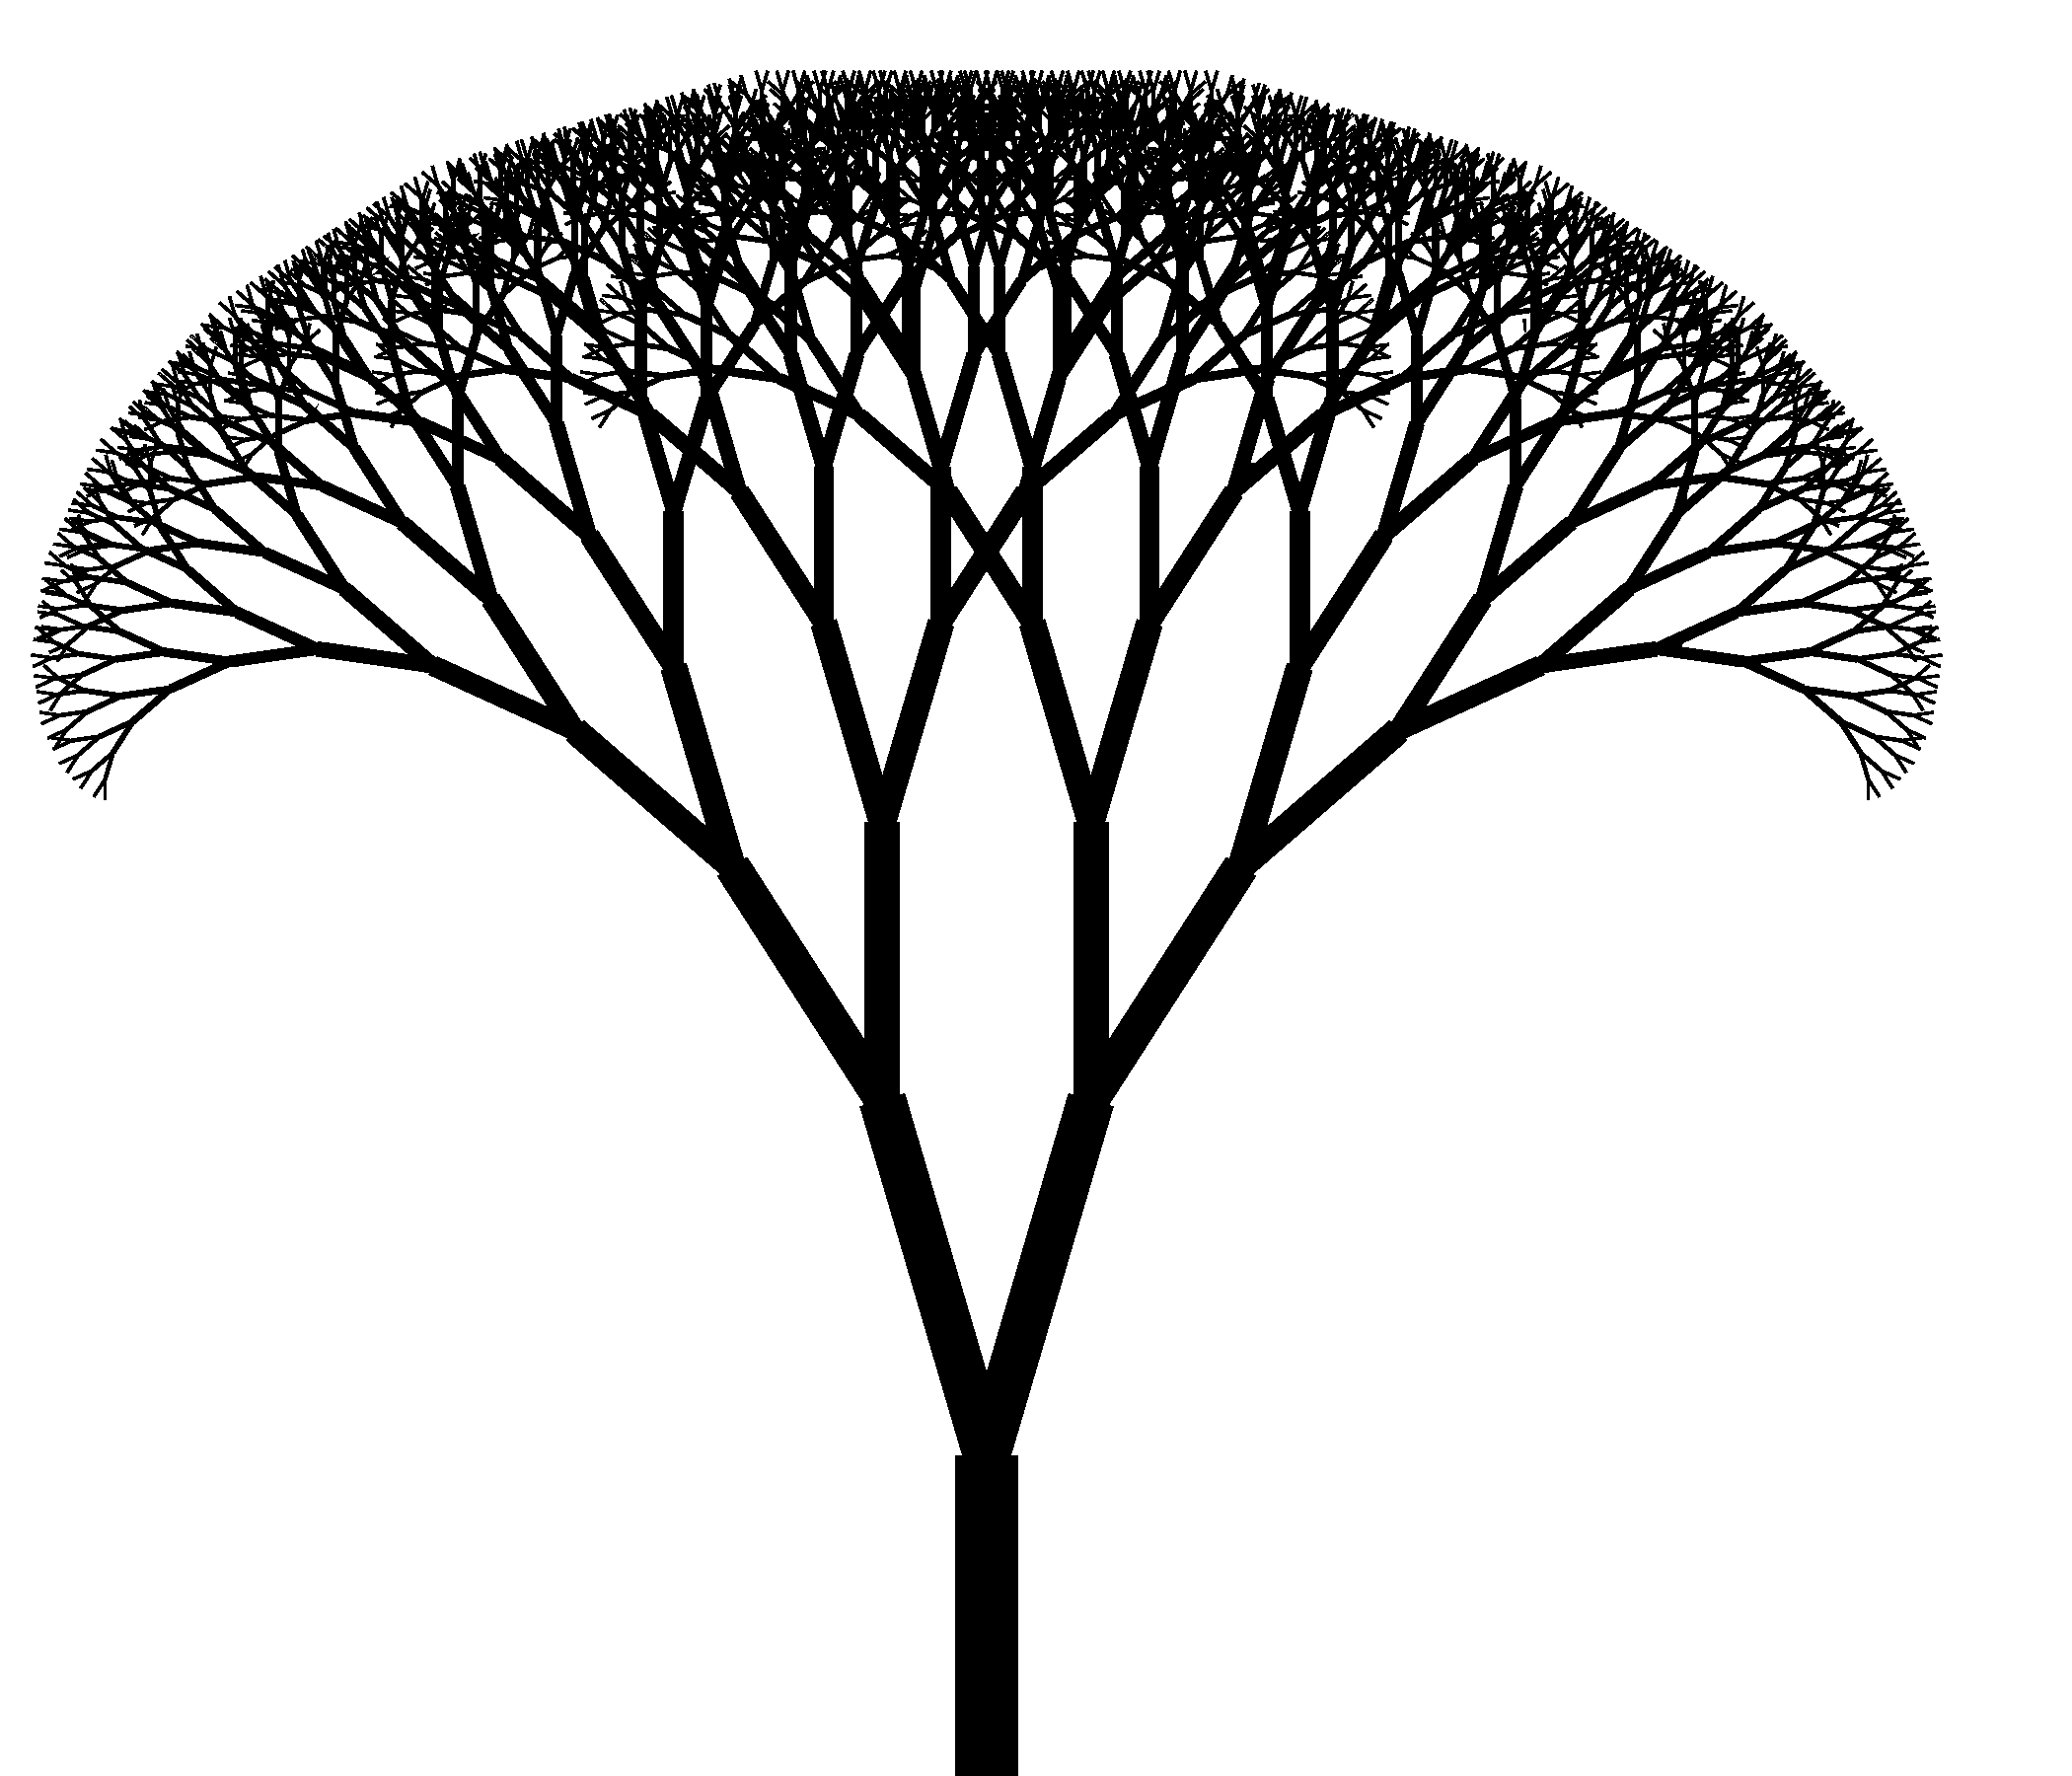
\includegraphics[width=\textwidth]{appendixB/canopy.png}}
  \caption[2100x1800 pixel canopy]{2100x1800 pixel canopy}
  \label{fig:canopy_png}
\end{figure}

\begin{figure}[!b]
  \centering
  \frame{
\includegraphics[width=\textwidth]{appendixB/fifty50.png}}
  \caption[2100x1800 pixel fifrty50]{2100x1800 pixel fifrty50}
  \label{fig:fifty50_png}
\end{figure}

\begin{figure}[!b]
  \centering
  \frame{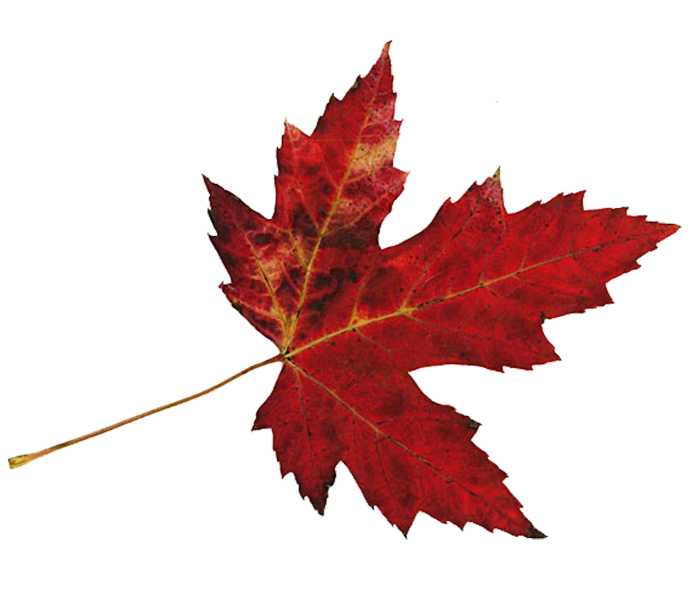
\includegraphics[width=\textwidth]{appendixB/fallleaf_fig.png}}
  \caption[2100x1800 pixel fallleaf]{2100x1800 pixel fallleaf - natural image prior to filtering}
  \label{fig:fallleaf_bmp}
\end{figure}

\begin{figure}[!b]
  \centering
  \frame{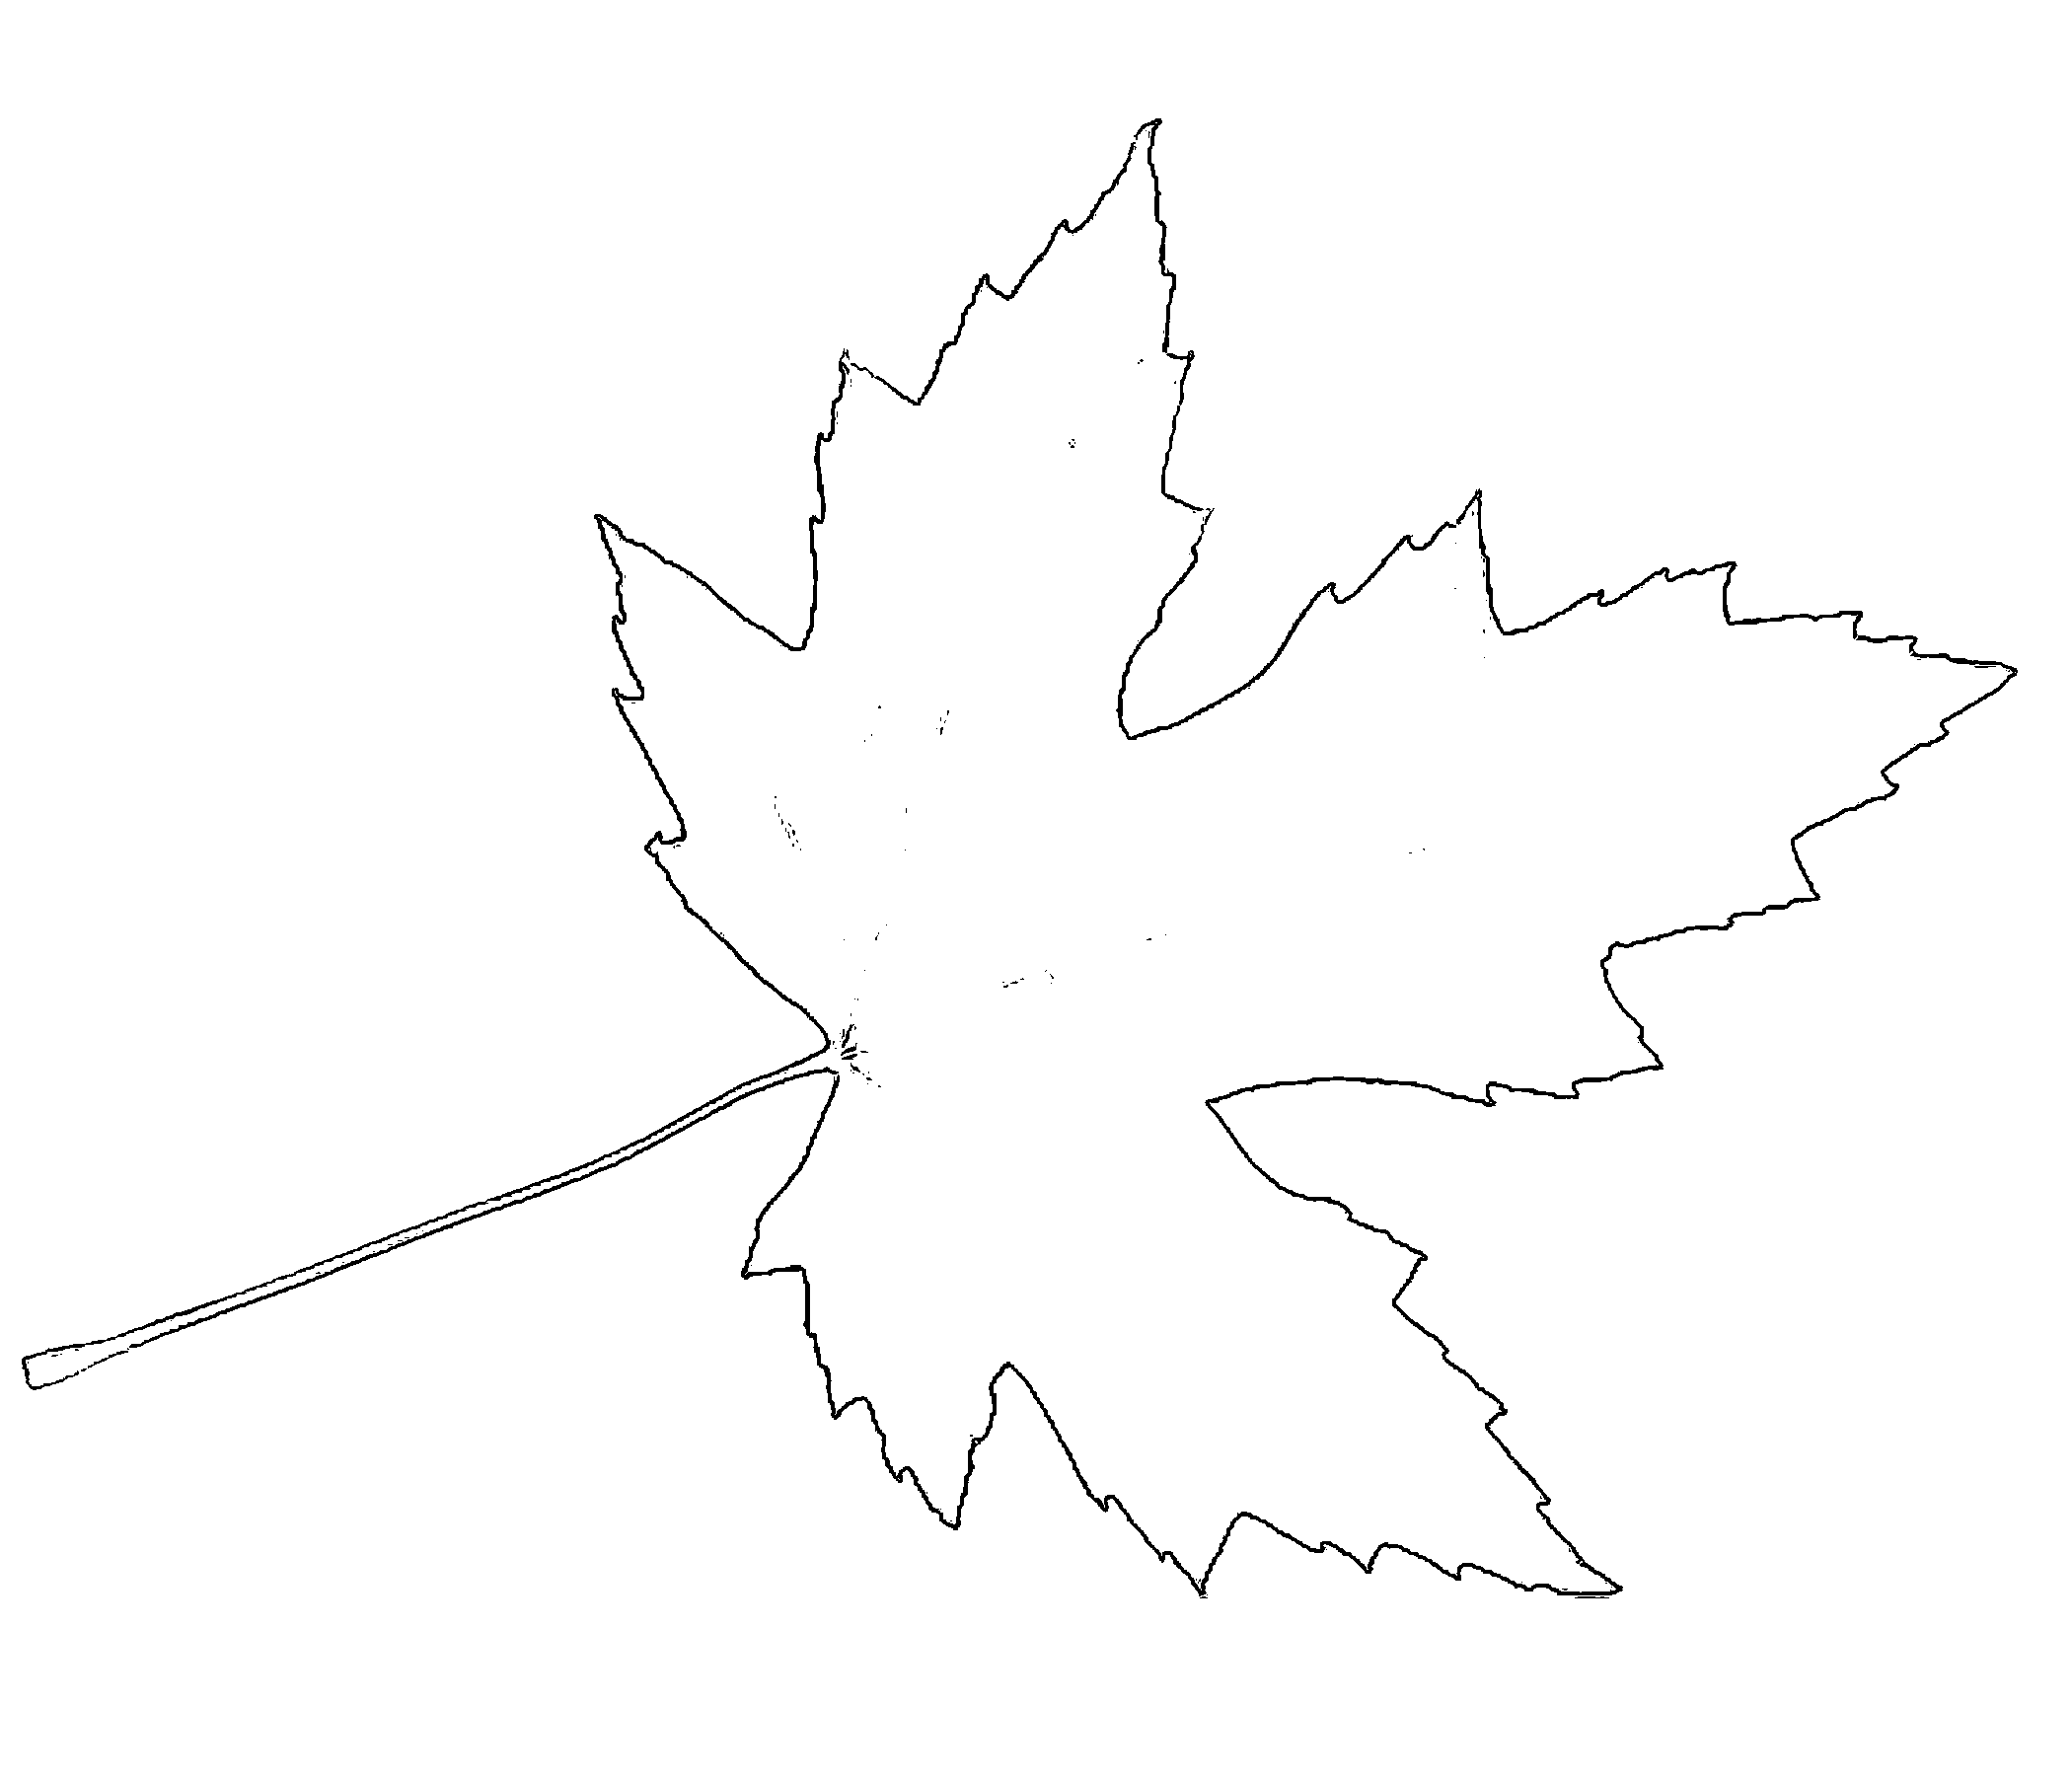
\includegraphics[width=\textwidth]{appendixB/20fallleaf.png}}
  \caption[2100x1800 pixel 20fallleaf]{2100x1800 pixel 20fallleaf - edge detect filtered at threshold level of 20}
  \label{fig:20fallleaf_png}
\end{figure}

\begin{figure}[!b]
  \centering
  \frame{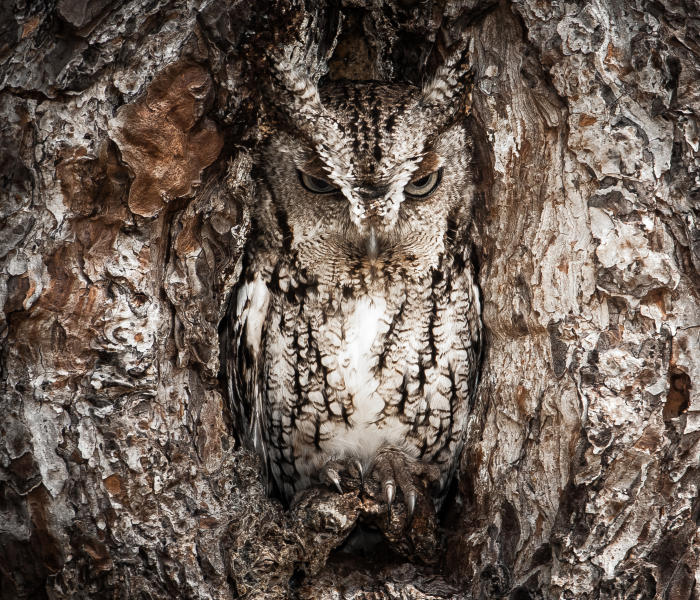
\includegraphics[width=\textwidth]{appendixB/owl_fig.png}}
  \caption[2100x1800 pixel owl]{2100x1800 pixel owl - natural image prior to filtering}
  \label{fig:owl_bmp}
\end{figure}

\begin{figure}[!b]
  \centering
  \frame{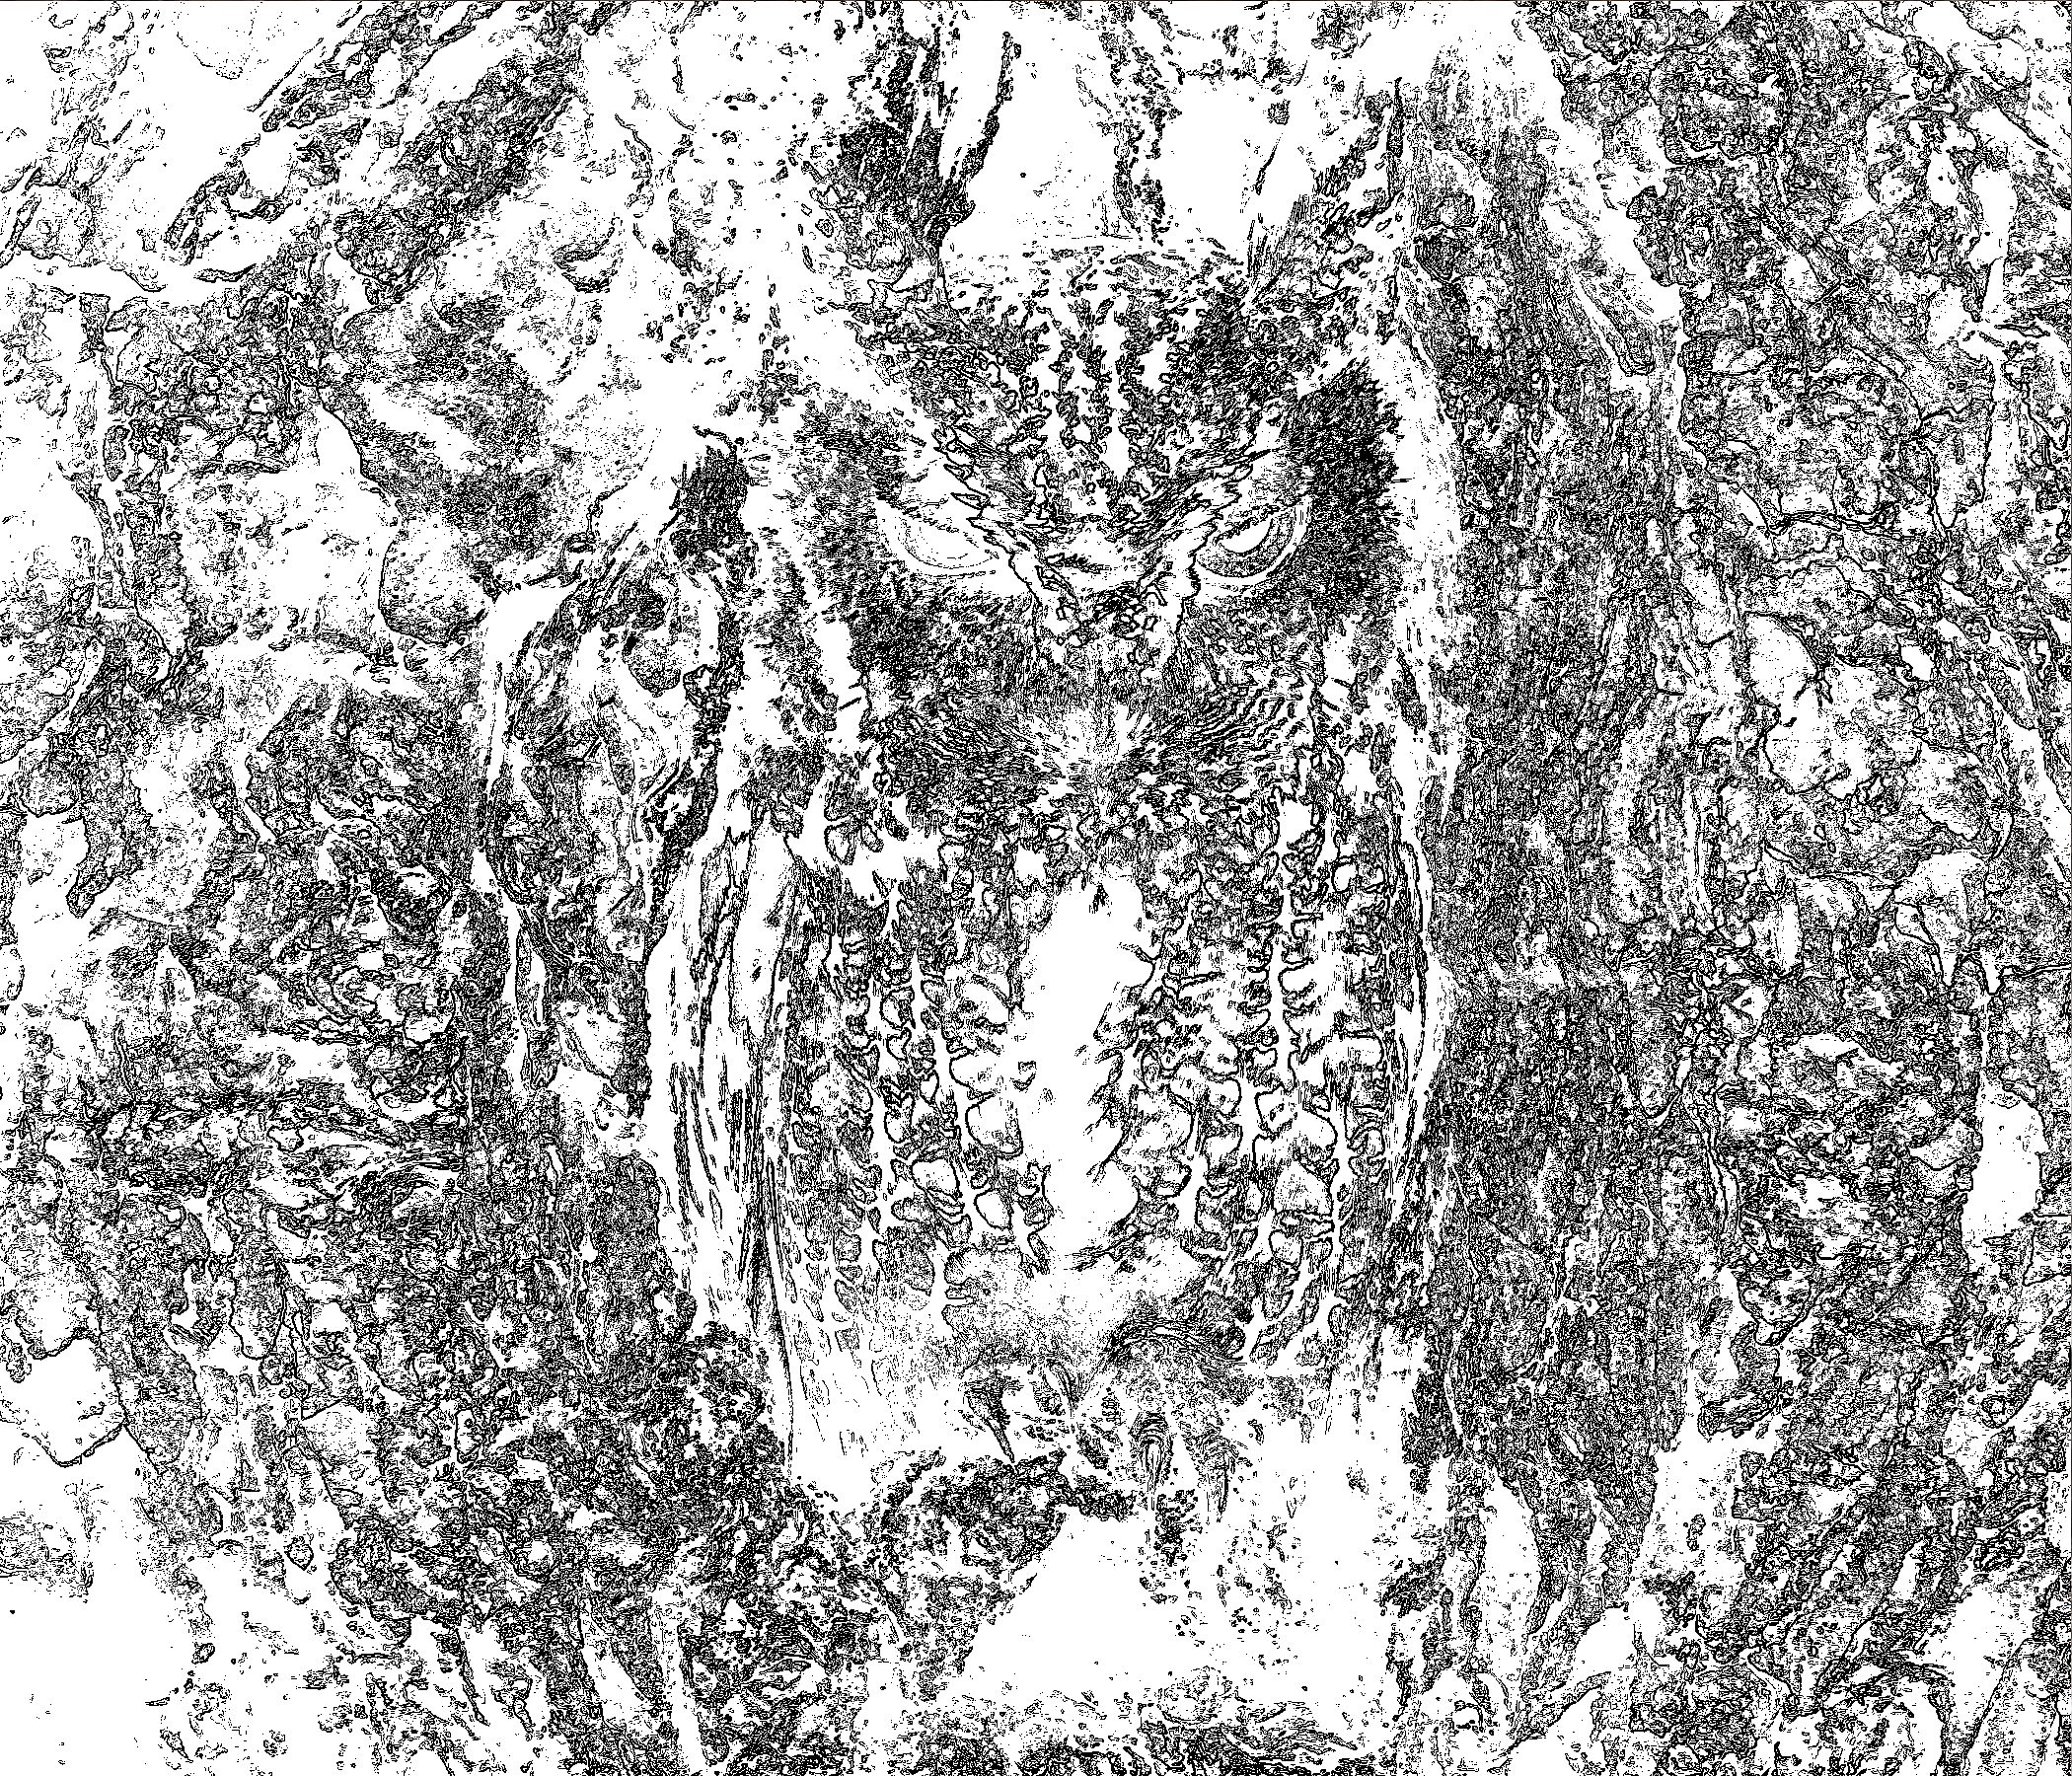
\includegraphics[width=\textwidth]{appendixB/20owl.png}}
  \caption[2100x1800 pixel 20owl]{2100x1800 pixel 20owl - edge detect filtered at threshold level of 20}
  \label{fig:20owl_png}
\end{figure}

\begin{figure}[!b]
  \centering
  \frame{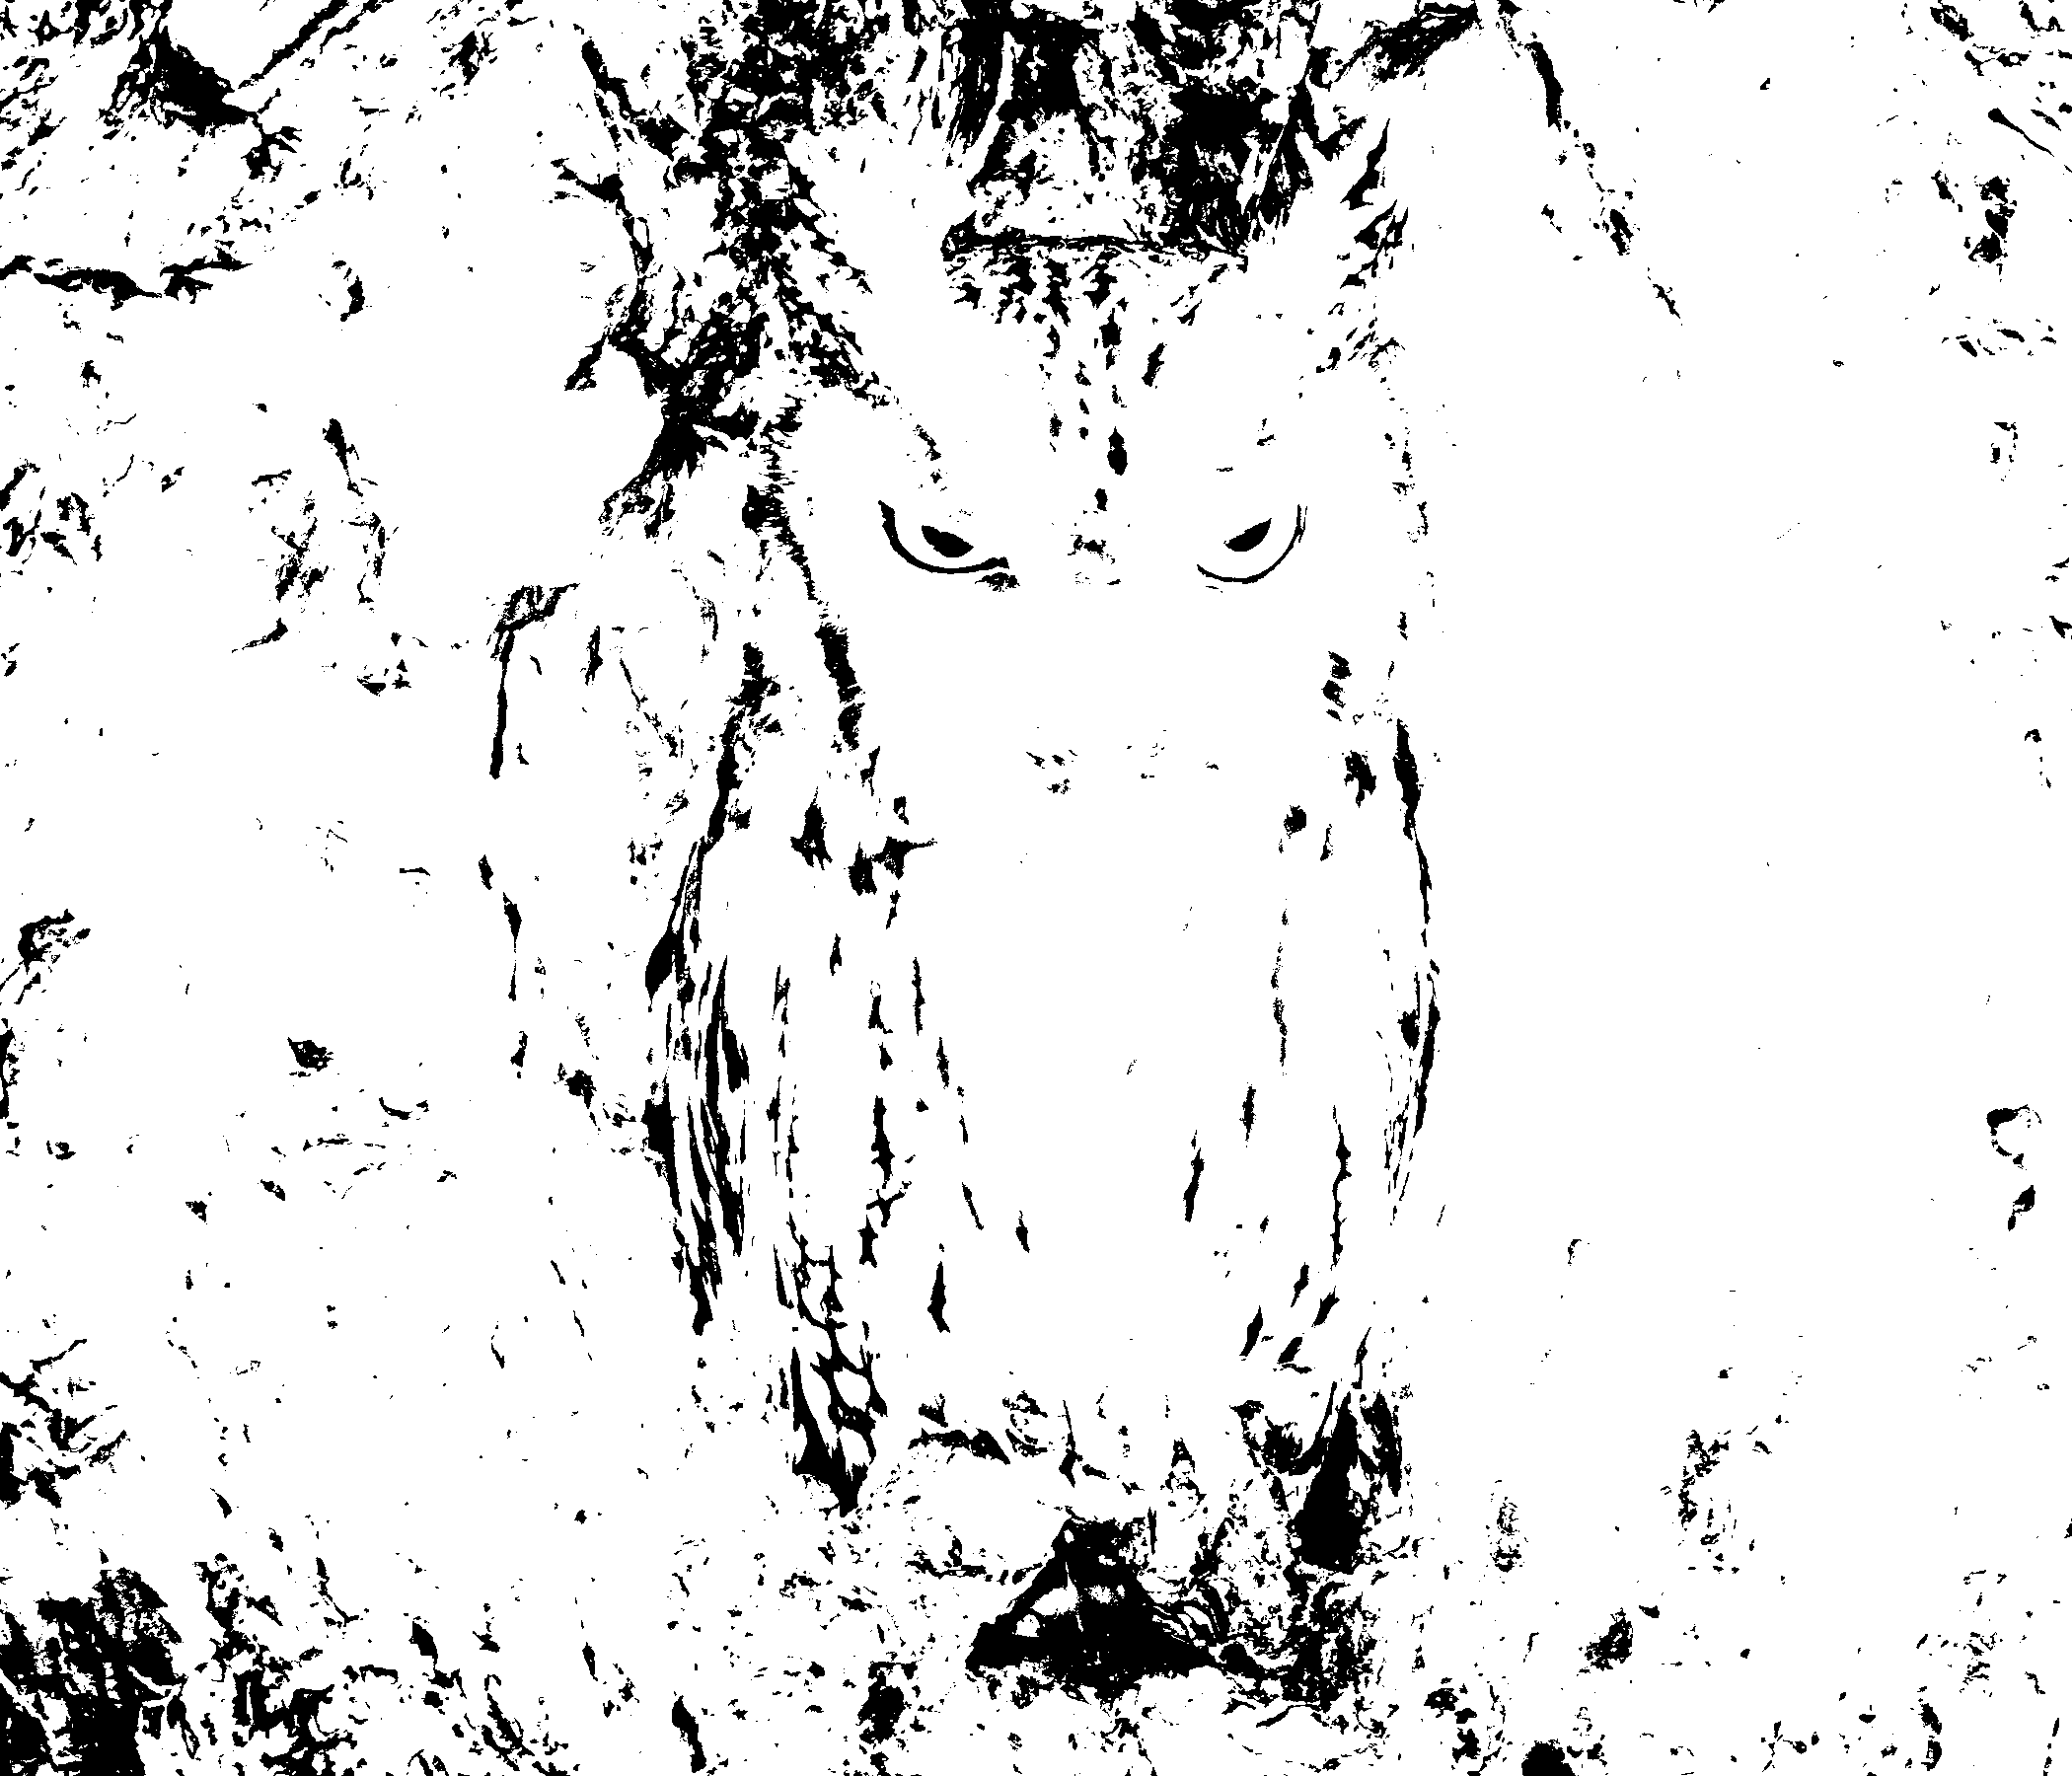
\includegraphics[width=\textwidth]{appendixB/20_thr_owl.png}}
  \caption[2100x1800 pixel 20throwl]{2100x1800 pixel 20throwl - threshold detect filtered at threshold level of 20}
  \label{fig:20thr_owl_png}
\end{figure}

\clearpage

% ================================================================
%
%  A P P E N D I X  C  - Uniform Results
% 
% ================================================================
\addcontentsline{toc}{chapter}{APPENDIX C - UNIFORM NOISE BCA RESULTS}
\begin{center}
\textbf{APPENDIX C}

\textbf{UNIFORM NOISE BCA RESULTS}
\end{center}

% Fig 32
\begin{figure}[!b]
  \centering
  \frame{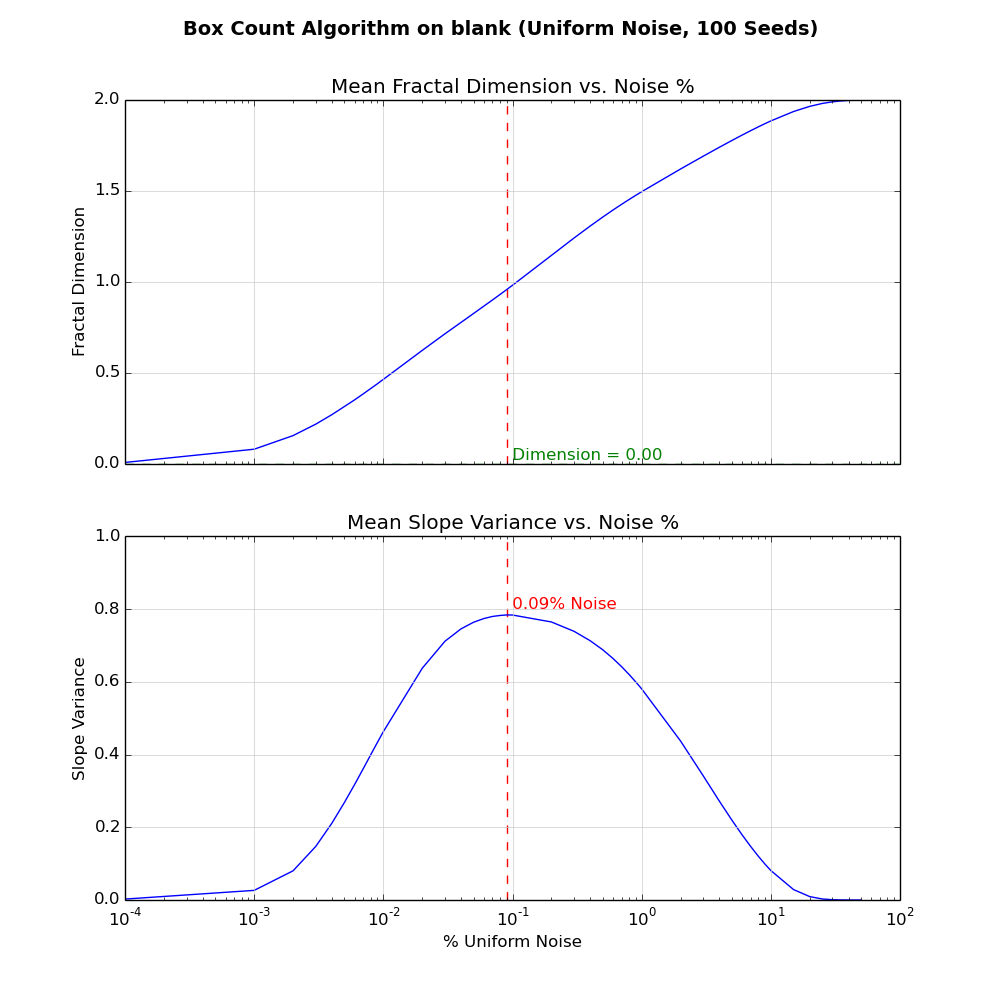
\includegraphics[width=\textwidth]{appendixC/Fig_Uniform_DvSV_blank.png}}
  \caption[Fractal Dimension and Slope Variance vs. Uniform noise for blank.png.]{Fractal Dimension and Slope Variance vs. Uniform noise for blank.png.  Results shown are the average of 100 noise seeds.  Highlighted are initial no-noise dimensional estimate, and Uniform Noise percentages where minimum dimension and maximum slope variance occur.}
  \label{fig:blank_uniform_result}
\end{figure}

\begin{figure}[!b]
  \centering
  \frame{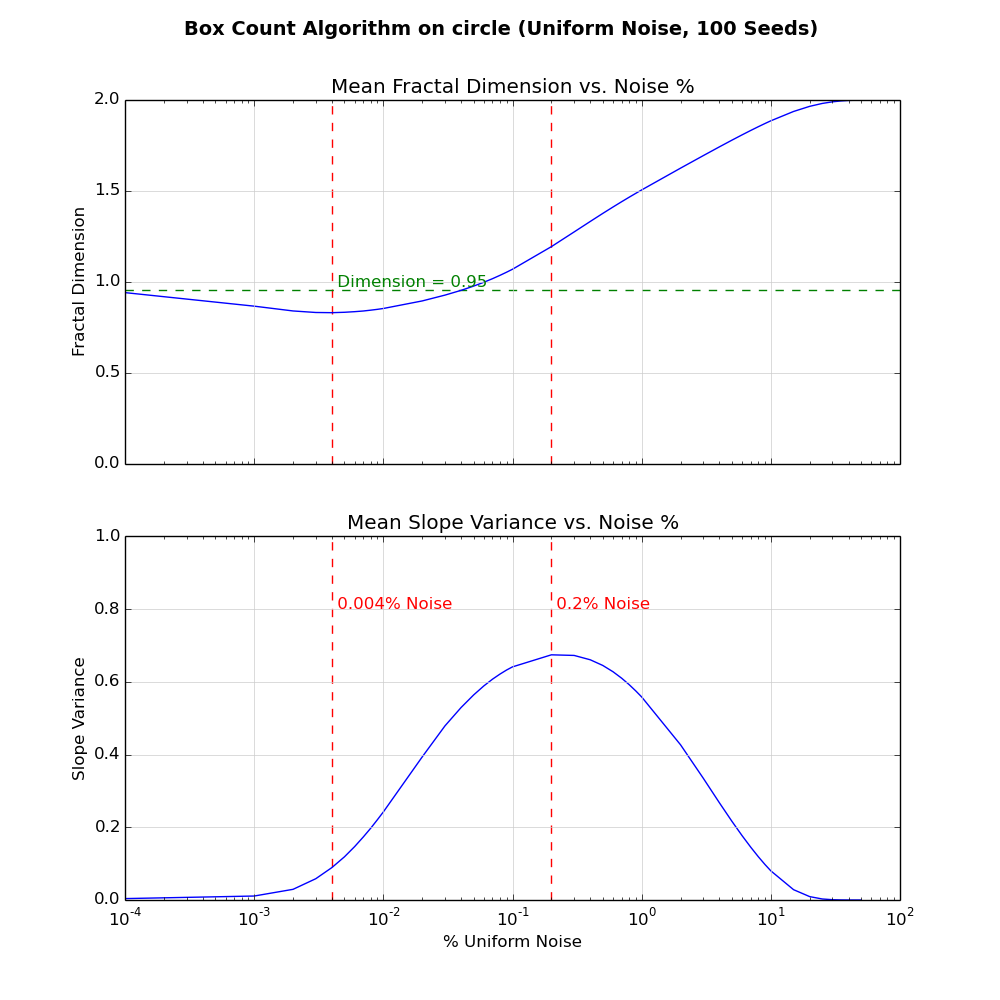
\includegraphics[width=\textwidth]{appendixC/Fig_Uniform_DvSV_circle.png}}
  \caption[Fractal Dimension and Slope Variance vs. Uniform noise for circle.png.]{Fractal Dimension and Slope Variance vs. Uniform noise for circle.png.  Results shown are the average of 100 noise seeds.  Highlighted are initial no-noise dimensional estimate, and Uniform Noise percentages where minimum dimension and maximum slope variance occur.}
  \label{fig:circle_uniform_result}
\end{figure}

\begin{figure}[!b]
  \centering
  \frame{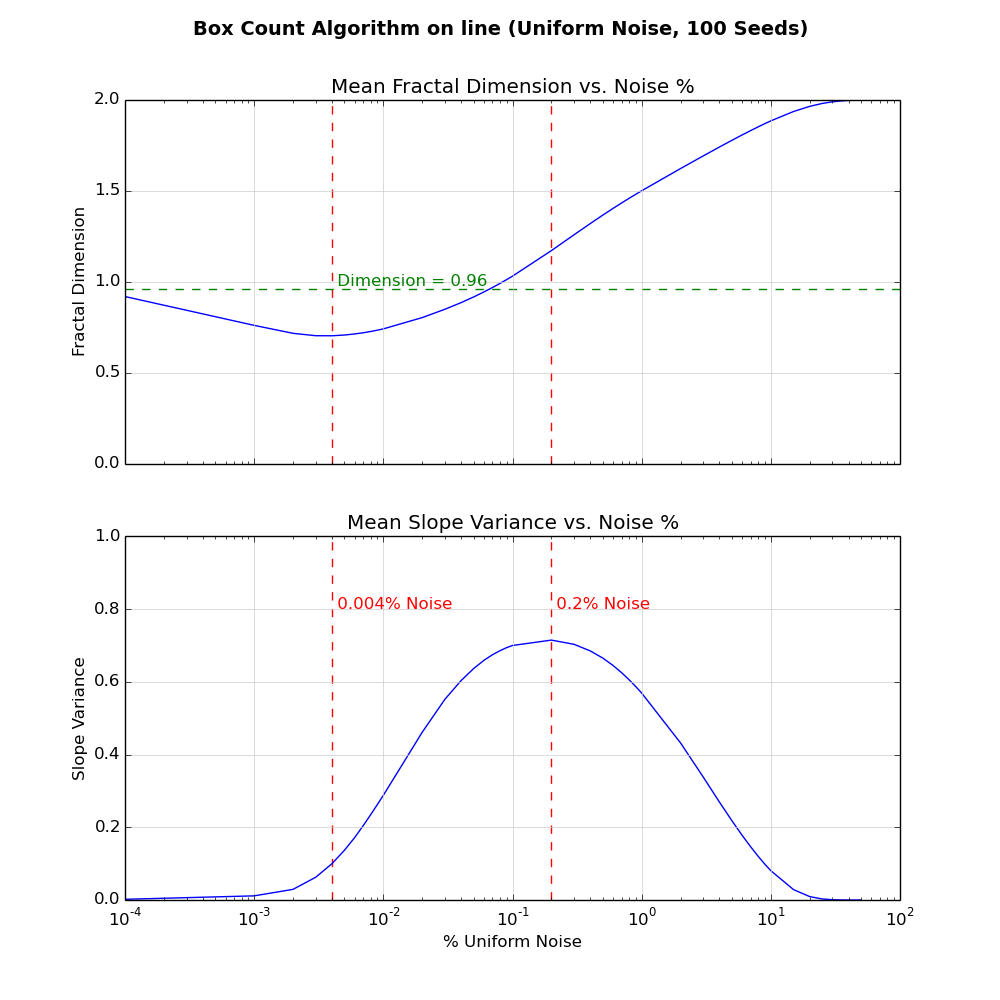
\includegraphics[width=\textwidth]{appendixC/Fig_Uniform_DvSV_line.png}}
  \caption[Fractal Dimension and Slope Variance vs. Uniform noise for line.png.]{Fractal Dimension and Slope Variance vs. Uniform noise for line.png.  Results shown are the average of 100 noise seeds.  Highlighted are initial no-noise dimensional estimate, and Uniform Noise percentages where minimum dimension and maximum slope variance occur.}
  \label{fig:line_uniform_result}
\end{figure}

\begin{figure}[!b]
  \centering
  \frame{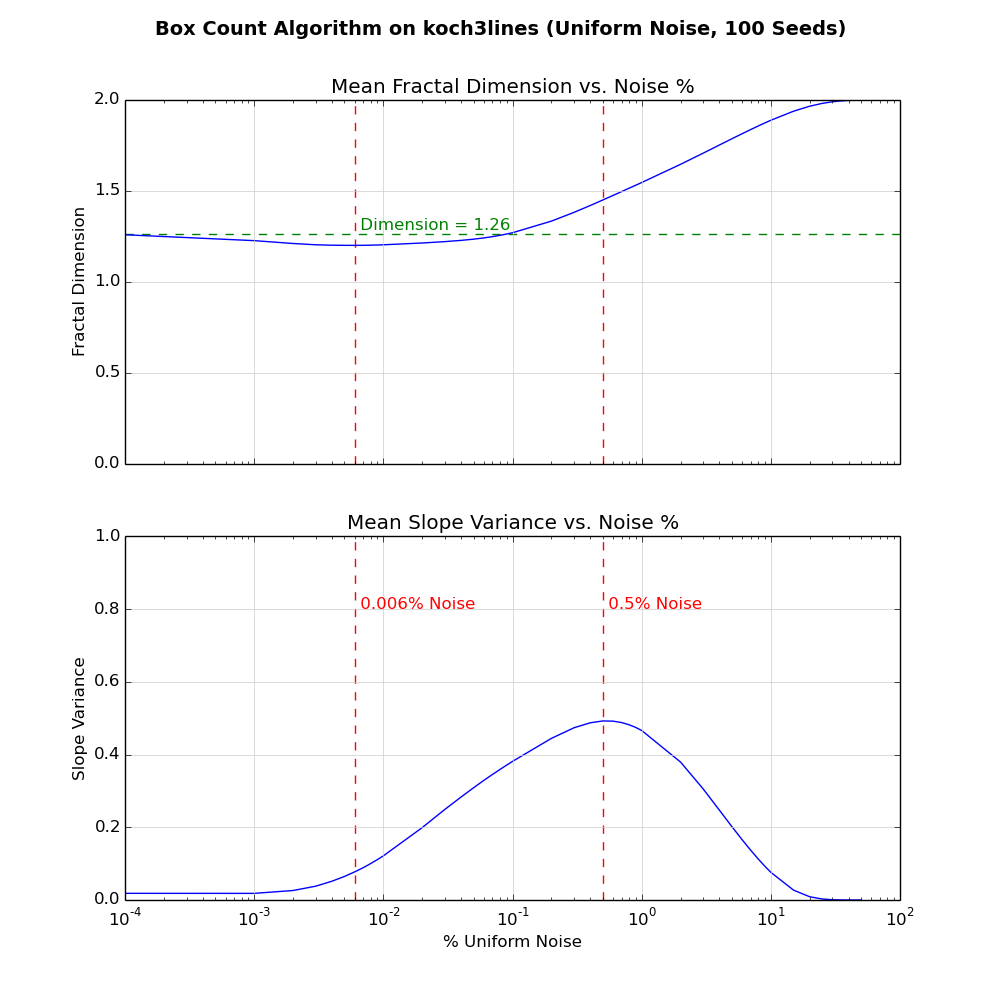
\includegraphics[width=\textwidth]{appendixC/Fig_Uniform_DvSV_koch3lines.png}}
  \caption[Fractal Dimension and Slope Variance vs. Uniform noise for koch3lines]{Fractal Dimension and Slope Variance vs. Uniform noise for koch3lines.png.  Results shown are the average of 100 noise seeds.  Highlighted are initial no-noise dimensional estimate, and Uniform Noise percentages where minimum dimension and maximum slope variance occur.}
  \label{fig:koch3lines_uniform_result}
\end{figure}

\begin{figure}[!b]
  \centering
  \frame{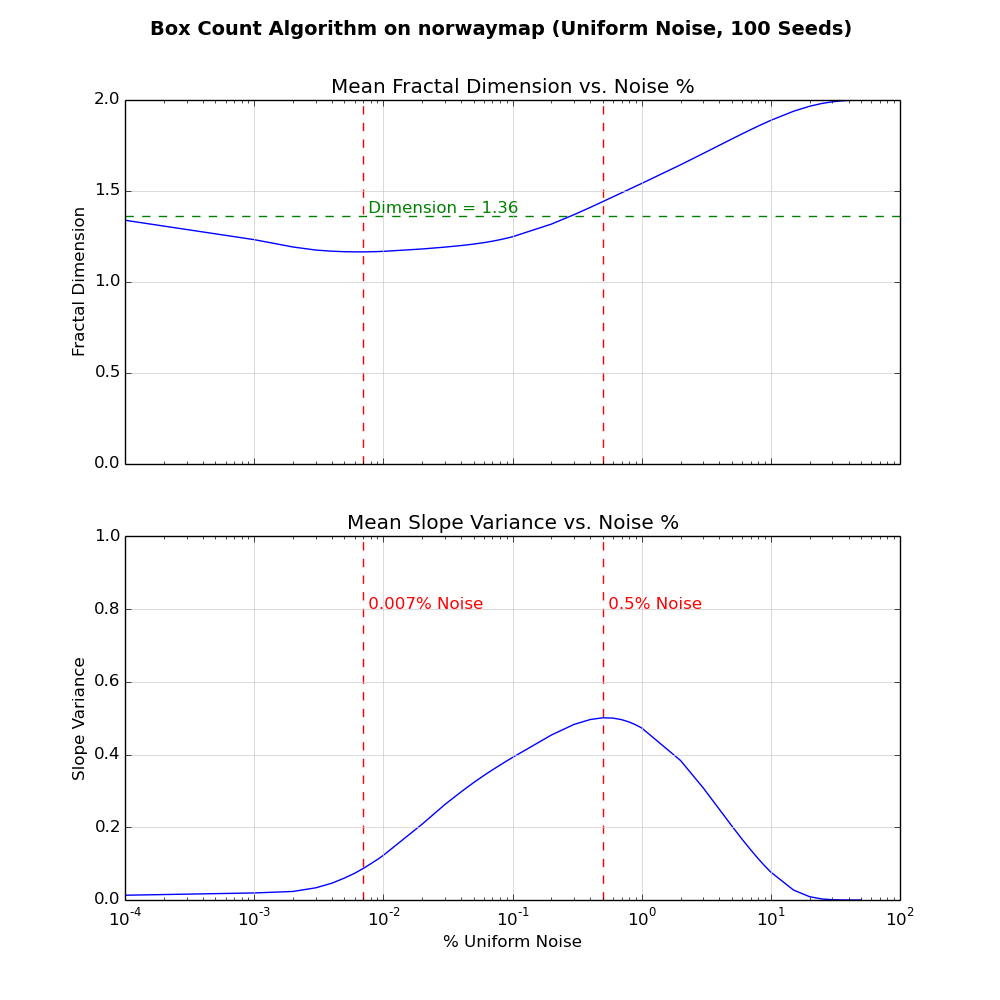
\includegraphics[width=\textwidth]{appendixC/Fig_Uniform_DvSV_norwaymap.png}}
  \caption[Fractal Dimension and Slope Variance vs. Uniform noise for norwaymap.png.]{Fractal Dimension and Slope Variance vs. Uniform noise for norwaymap.png.  Results shown are the average of 100 noise seeds.  Highlighted are initial no-noise dimensional estimate, and Uniform Noise percentages where minimum dimension and maximum slope variance occur.}
  \label{fig:norwaymap_uniform_result}
\end{figure}

\begin{figure}[!b]
  \centering
  \frame{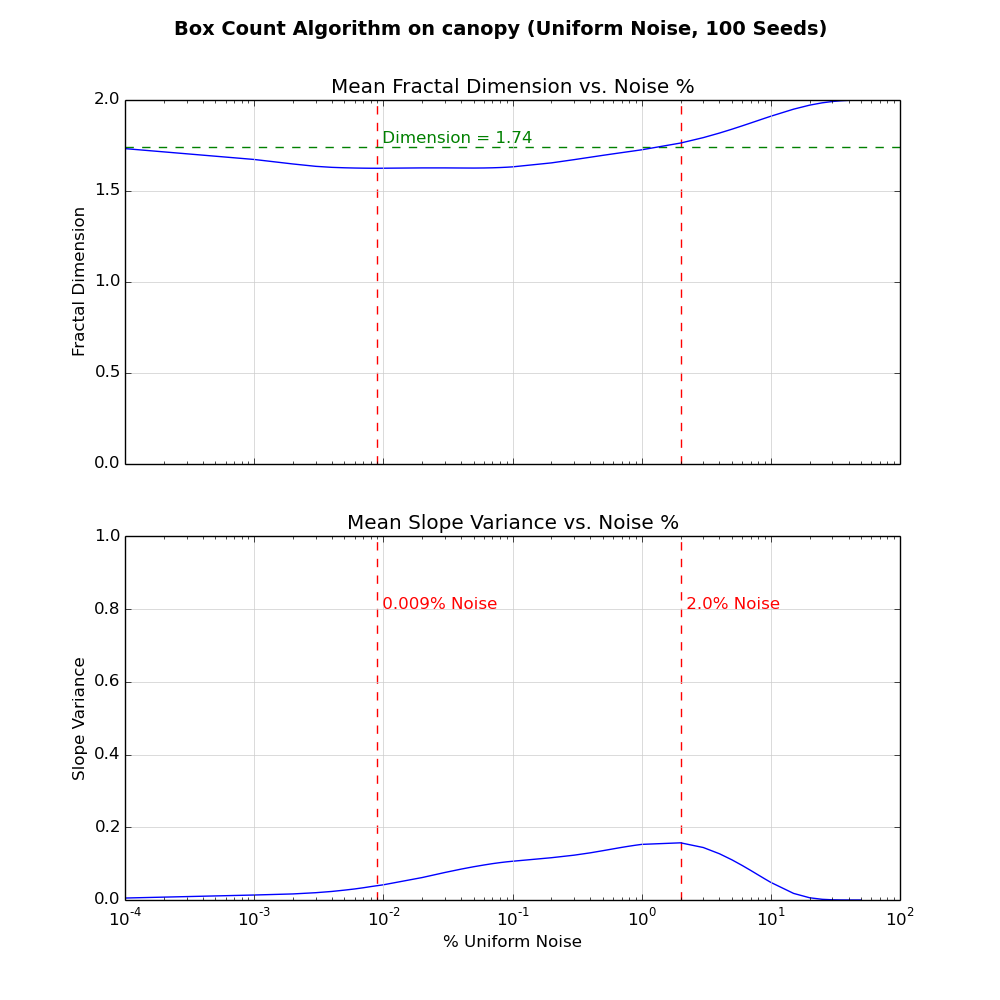
\includegraphics[width=\textwidth]{appendixC/Fig_Uniform_DvSV_canopy.png}}
  \caption[Fractal Dimension and Slope Variance vs. Uniform noise for canopy.png]{Fractal Dimension and Slope Variance vs. Uniform noise for canopy.png.  Results shown are the average of 100 noise seeds.  Highlighted are initial no-noise dimensional estimate, and Uniform Noise percentages where minimum dimension and maximum slope variance occur.}
  \label{fig:canopy_uniform_result}
\end{figure}

\begin{figure}[!b]
  \centering
  \frame{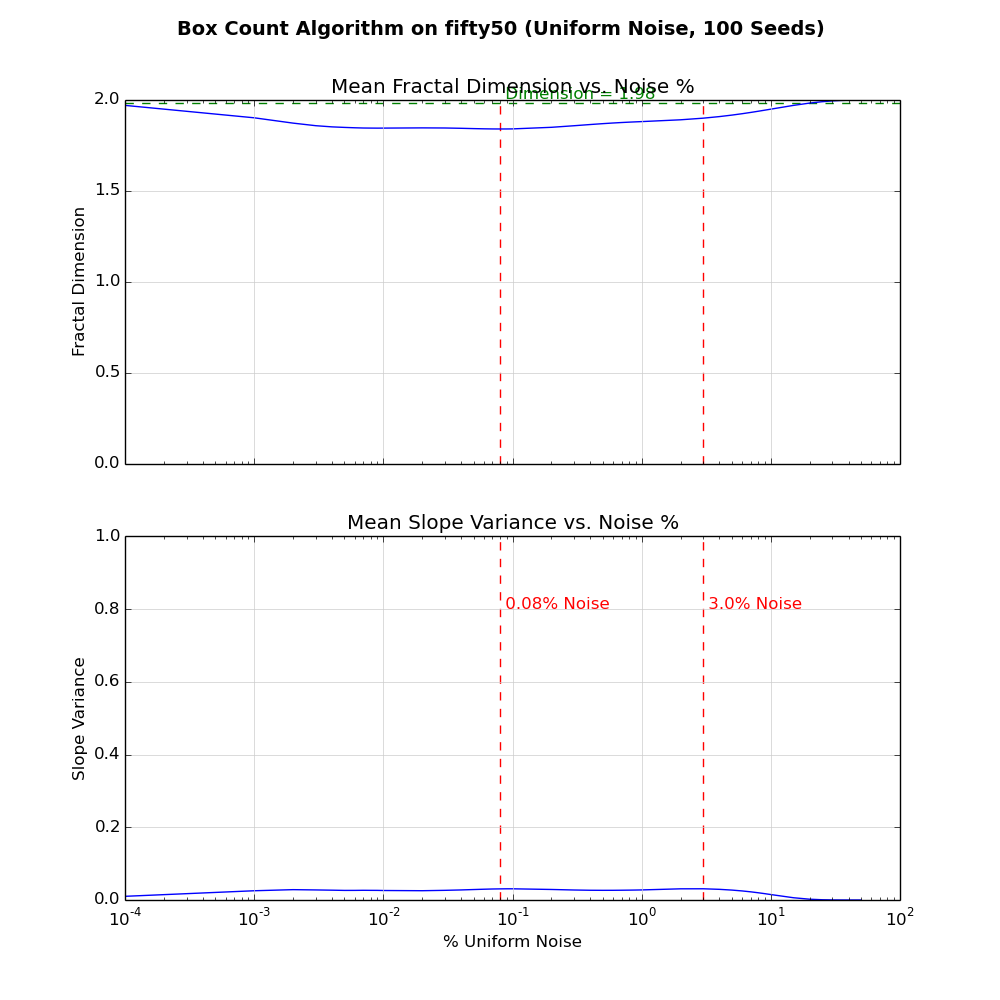
\includegraphics[width=\textwidth]{appendixC/Fig_Uniform_DvSV_fifty50.png}}
  \caption[Fractal Dimension and Slope Variance vs. Uniform noise for fifty50.png.]{Fractal Dimension and Slope Variance vs. Uniform noise for fifty50.png.  Results shown are the average of 100 noise seeds.  Highlighted are initial no-noise dimensional estimate, and Uniform Noise percentages where minimum dimension and maximum slope variance occur.}
  \label{fig:fifty50_uniform_result}
\end{figure}

%Fig 39 
\begin{figure}[!b]
  \centering
  \frame{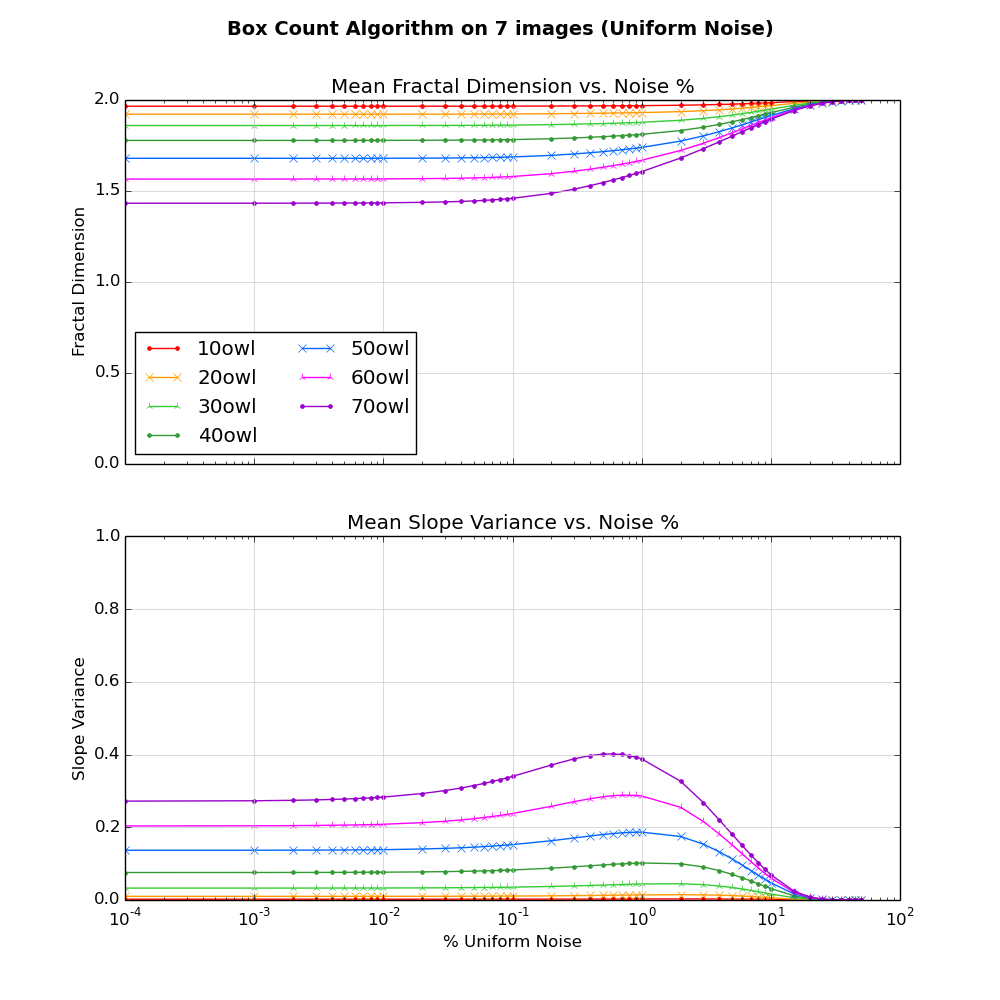
\includegraphics[width=\textwidth]{appendixC/Fig_DvsSV_Uniform_Multiplot_70owl.png}}
  \caption[Fractal Dimension and Slope Variance vs. Uniform noise for the owl edge-detection selected set]{Fractal Dimension and Slope Variance vs. Uniform noise for the owl edge-detection selected set.}
  \label{fig:owl-ed_multi_uniform_result}
\end{figure}

%Fig 40
\begin{figure}[!b]
  \centering
  \frame{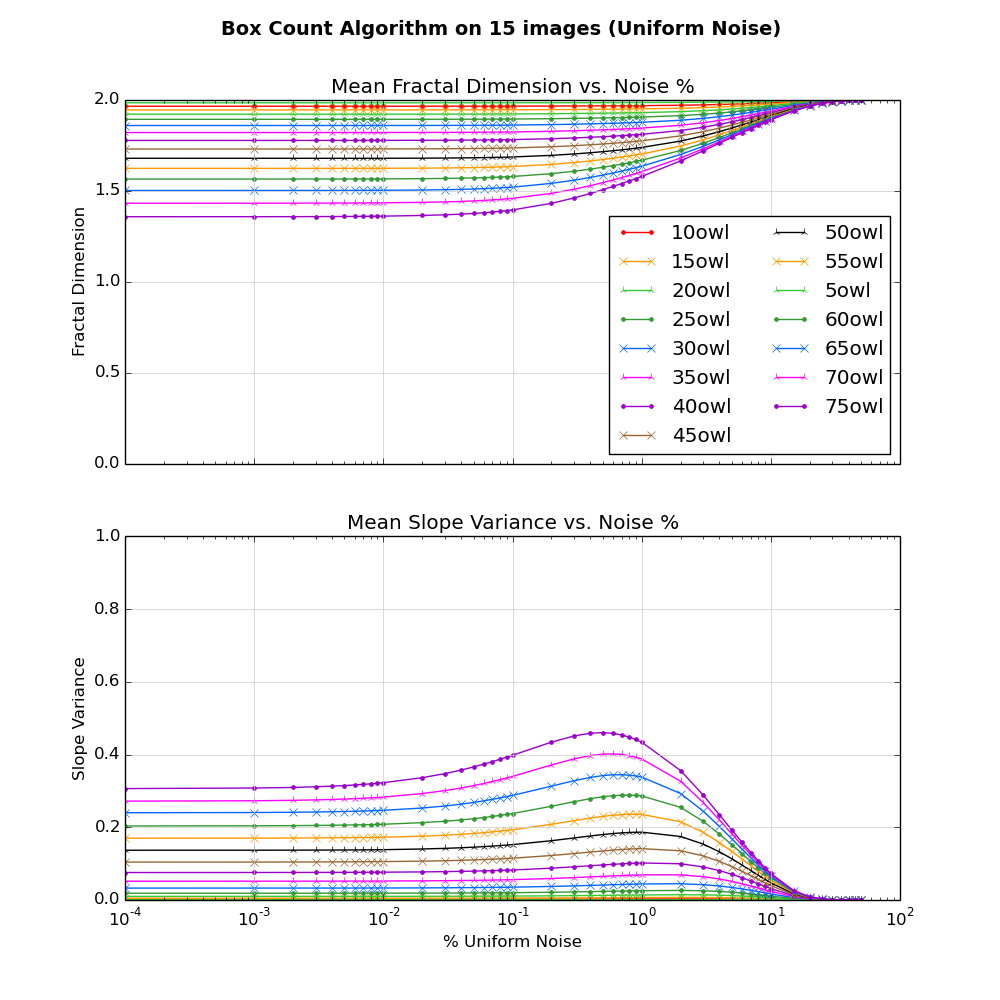
\includegraphics[width=\textwidth]{appendixC/Fig_DvsSV_Uniform_Multiplot_75owl.png}}
  \caption[Fractal Dimension and Slope Variance vs. Uniform noise for the owl edge-detection full set]{Fractal Dimension and Slope Variance vs. Uniform noise for the owl edge-detection full set.}
  \label{fig:owl-ed2_multi_uniform_result}
\end{figure}

\begin{figure}[!b]
  \centering
  \frame{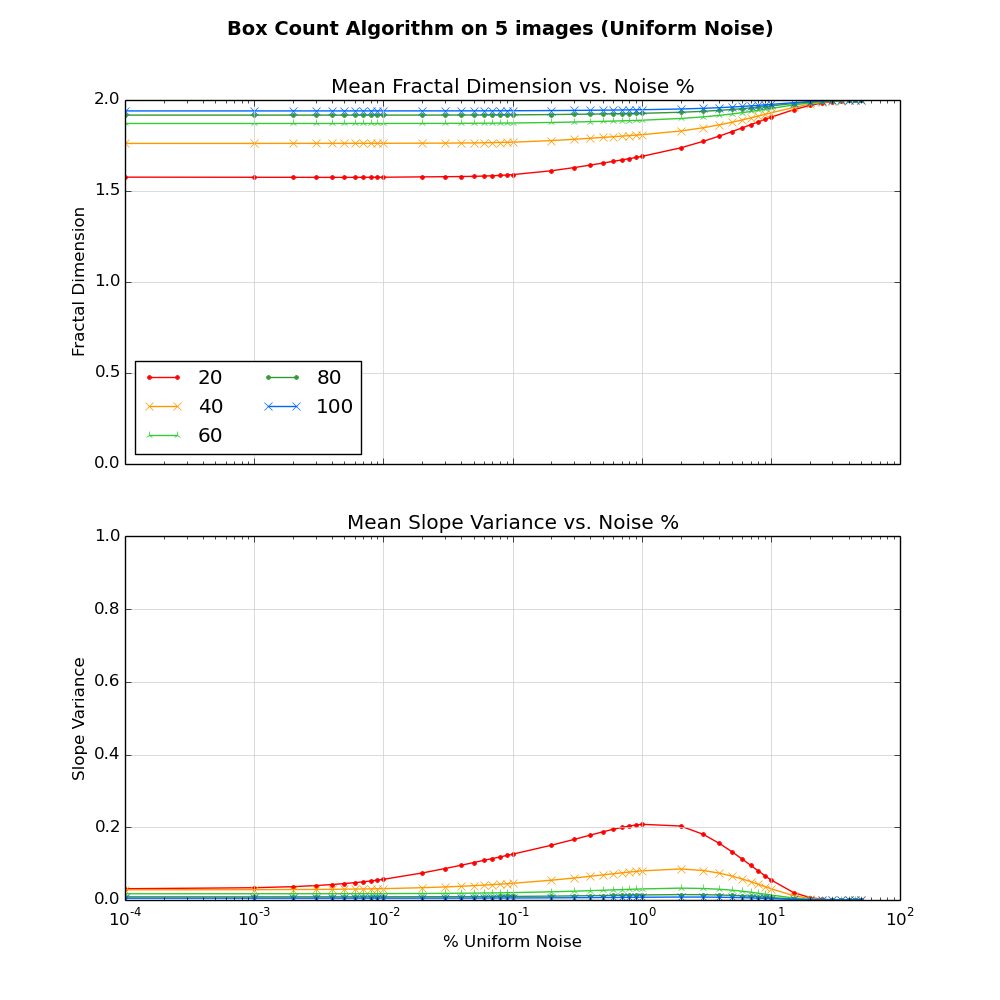
\includegraphics[width=\textwidth]{appendixC/Fig_DvsSV_Uniform_Multiplot_100.png}}
  \caption[Fractal Dimension and Slope Variance vs. Uniform noise for the owl threshold-detection selected set]{Fractal Dimension and Slope Variance vs. Uniform noise for the owl threshold-detection selected set.}
  \label{fig:owl-thresh_multi_uniform_result}
\end{figure}

\clearpage

% ================================================================
%
%  A P P E N D I X  D  - Gaussian Results
% 
% ================================================================
\addcontentsline{toc}{chapter}{APPENDIX D - GAUSSIAN NOISE BCA RESULTS}
\begin{center}
\textbf{APPENDIX D}

\textbf{GAUSSIAN NOISE BCA RESULTS}
\end{center}

%Fig 42
\begin{figure}[!b]
  \centering
  \frame{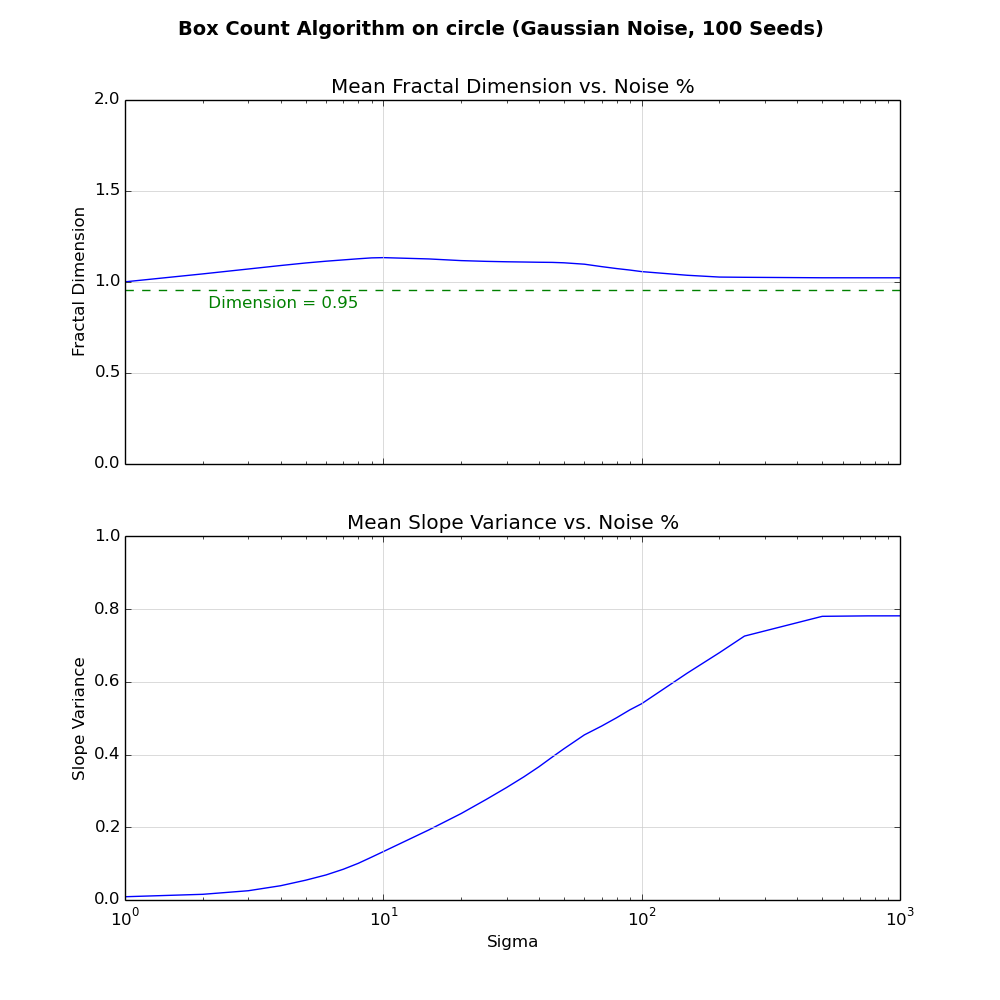
\includegraphics[width=\textwidth]{appendixD/Fig_Gaussian_DvSV_circle.png}}
  \caption[Fractal Dimension and Slope Variance vs. Gaussian noise for circle.png.]{Fractal Dimension and Slope Variance vs. Gaussian noise for circle.png.  Results shown are the average of 100 noise seeds.  Highlighted is initial no-noise dimensional estimate.}
  \label{fig:circle_gaussian_result}
\end{figure}

\begin{figure}[!b]
  \centering
  \frame{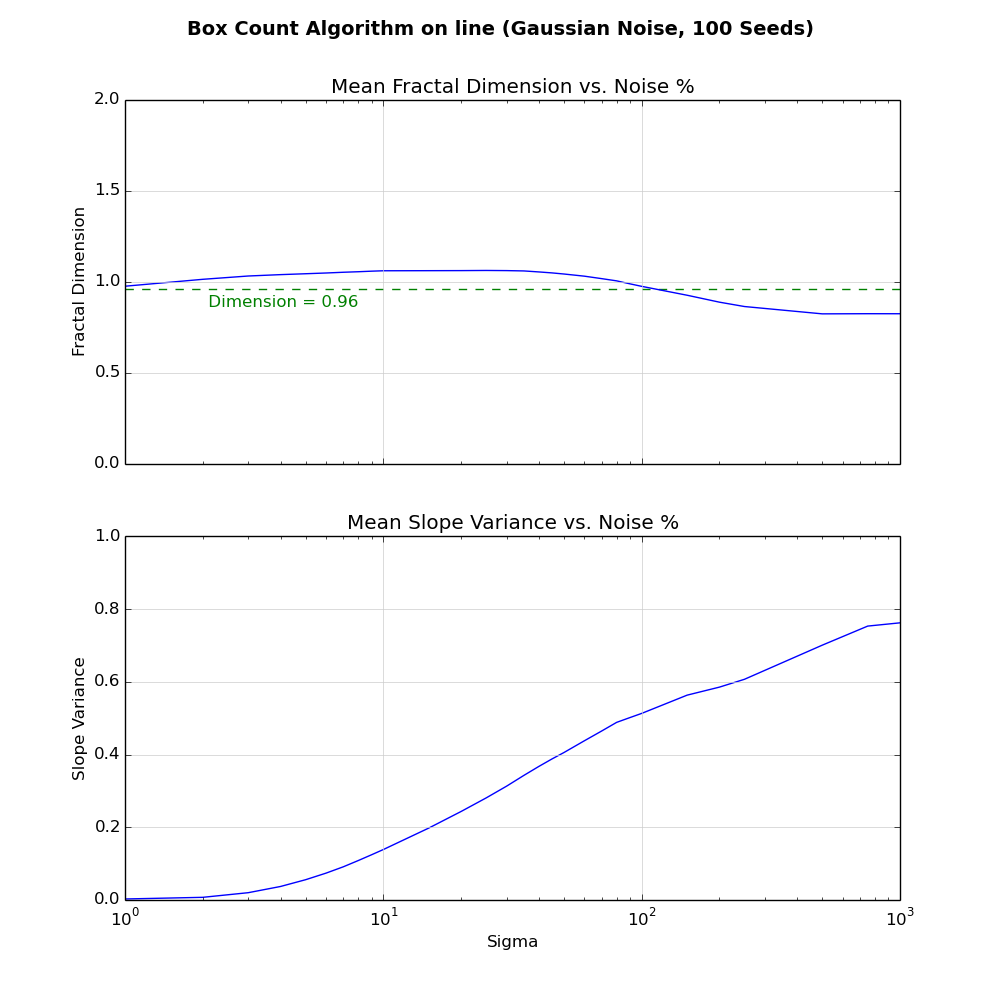
\includegraphics[width=\textwidth]{appendixD/Fig_Gaussian_DvSV_line.png}}
  \caption[Fractal Dimension and Slope Variance vs. Gaussian noise for line.png.]{Fractal Dimension and Slope Variance vs. Gaussian noise for line.png.  Results shown are the average of 100 noise seeds.  Highlighted is initial no-noise dimensional estimate.}
  \label{fig:line_gaussian_result}
\end{figure}

\begin{figure}[!b]
  \centering
  \frame{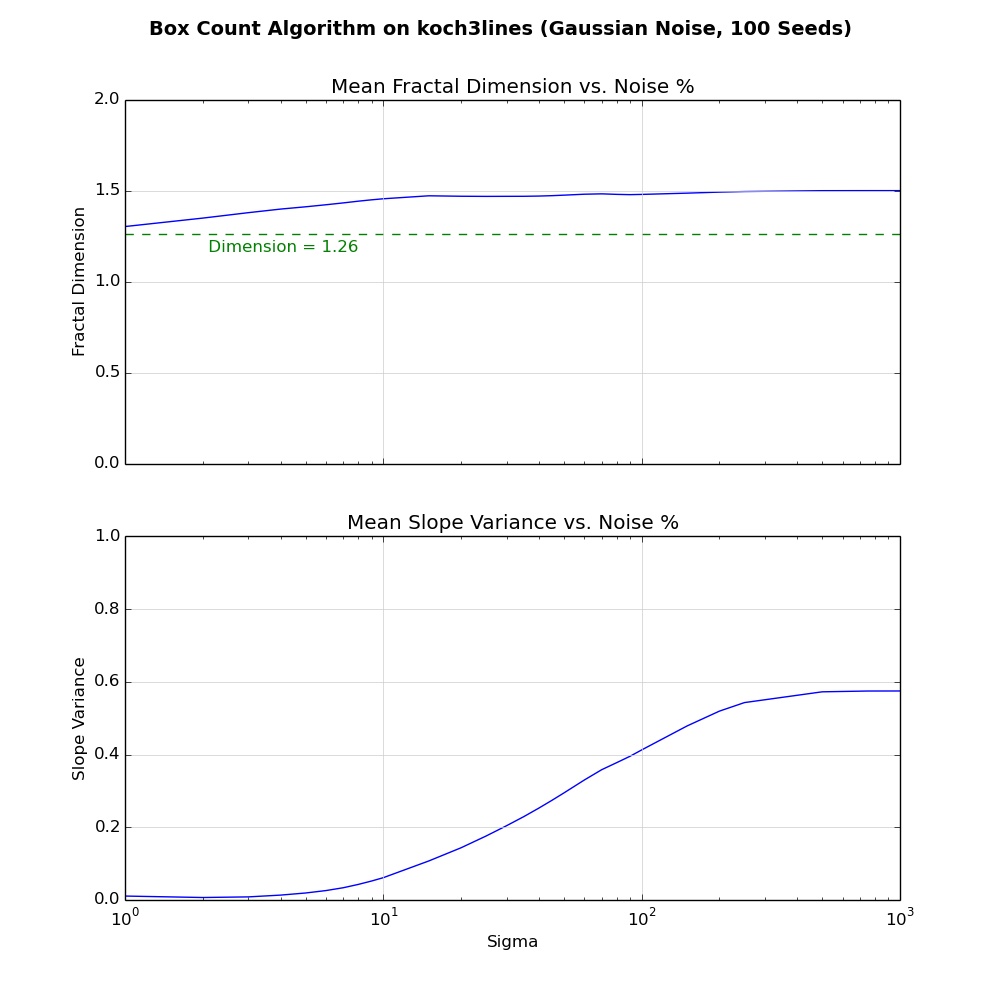
\includegraphics[width=\textwidth]{appendixD/Fig_Gaussian_DvSV_koch3lines.png}}
  \caption[Fractal Dimension and Slope Variance vs. Gaussian noise for koch3lines.png.]{Fractal Dimension and Slope Variance vs. Gaussian noise for koch3lines.png.  Results shown are the average of 100 noise seeds.  Highlighted is initial no-noise dimensional estimate.}
  \label{fig:koch3lines_gaussian_result}
\end{figure}

%Fig 45
\begin{figure}[!b]
  \centering
  \frame{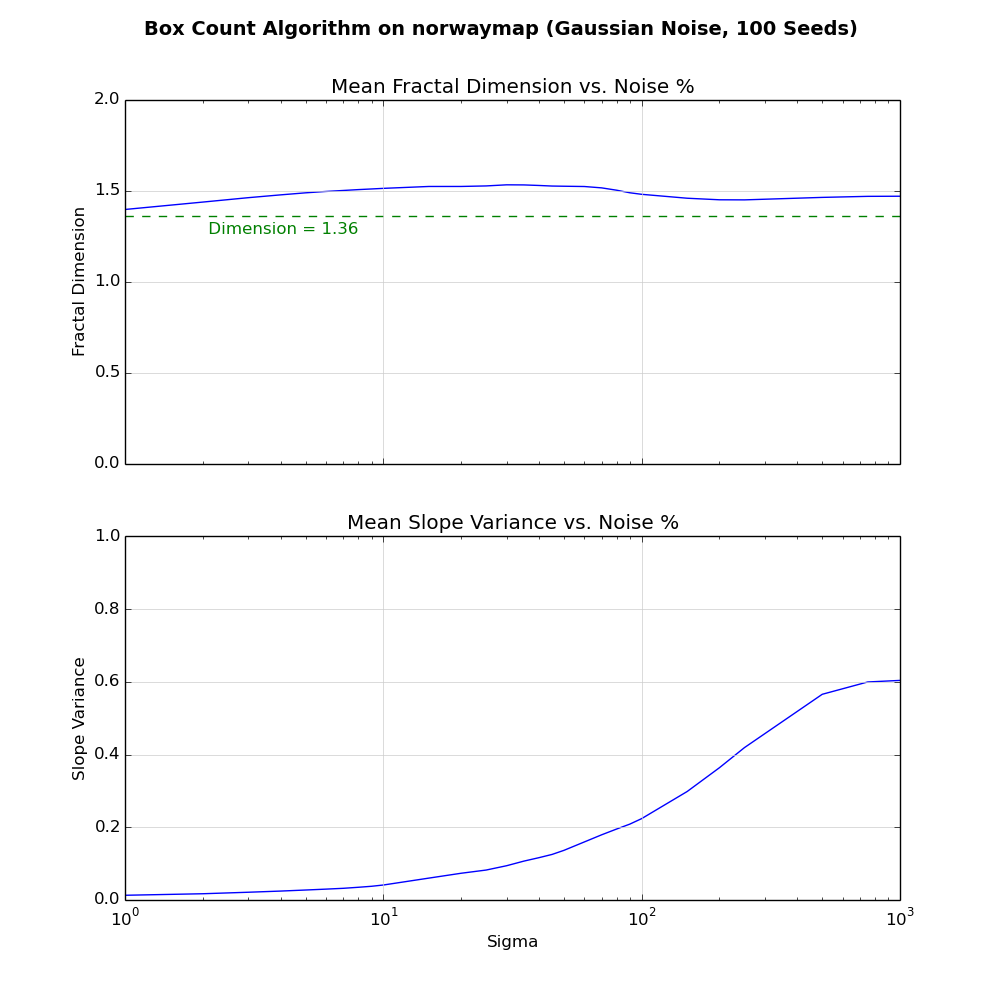
\includegraphics[width=\textwidth]{appendixD/Fig_Gaussian_DvSV_norwaymap.png}}
  \caption[Fractal Dimension and Slope Variance vs. Gaussian noise for norwaymap.png.]{Fractal Dimension and Slope Variance vs. Gaussian noise for norwaymap.png.  Results shown are the average of 100 noise seeds.  Highlighted is initial no-noise dimensional estimate.}
  \label{fig:norwaymap_gaussian_result}
\end{figure}

\begin{figure}[!b]
  \centering
  \frame{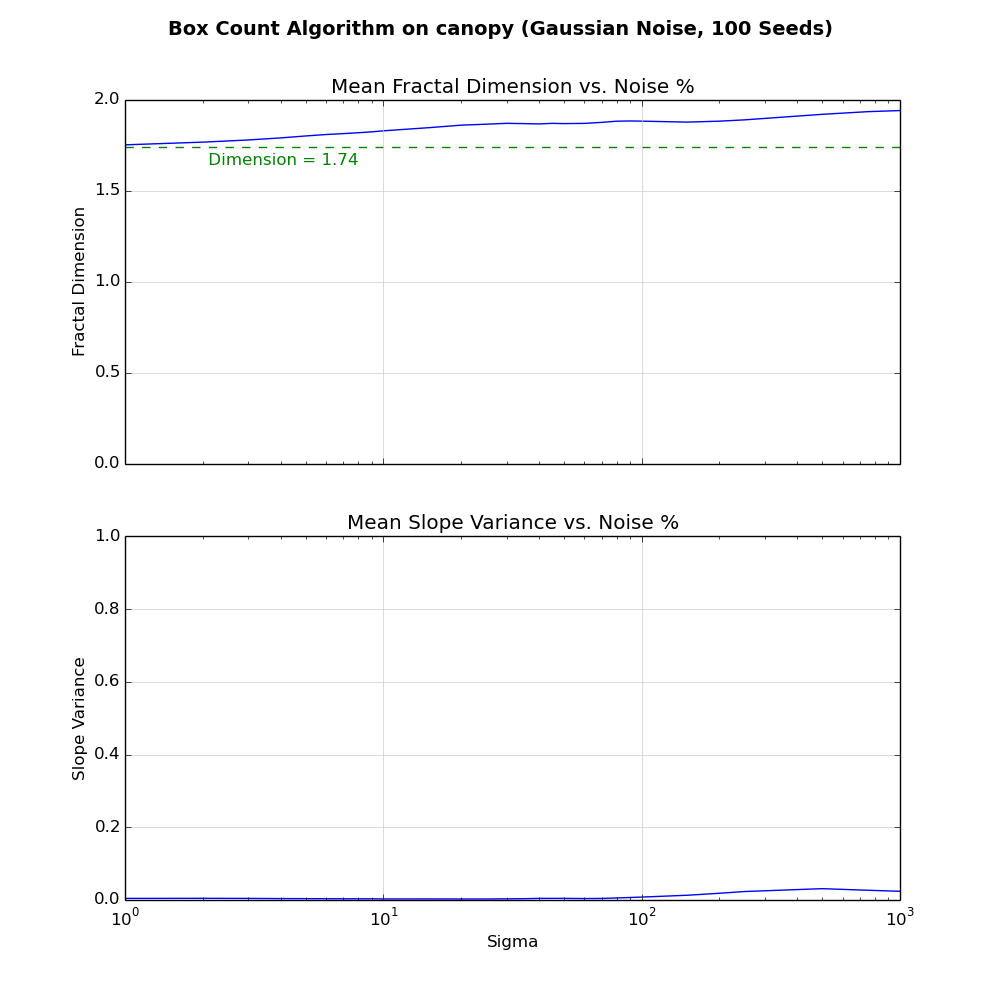
\includegraphics[width=\textwidth]{appendixD/Fig_Gaussian_DvSV_canopy.png}}
  \caption[Fractal Dimension and Slope Variance vs. Gaussian noise for canopy.png.]{Fractal Dimension and Slope Variance vs. Gaussian noise for canopy.png.  Results shown are the average of 100 noise seeds.  Highlighted is initial no-noise dimensional estimate.}
  \label{fig:canopy_gaussian_result}
\end{figure}

\begin{figure}[!b]
  \centering
  \frame{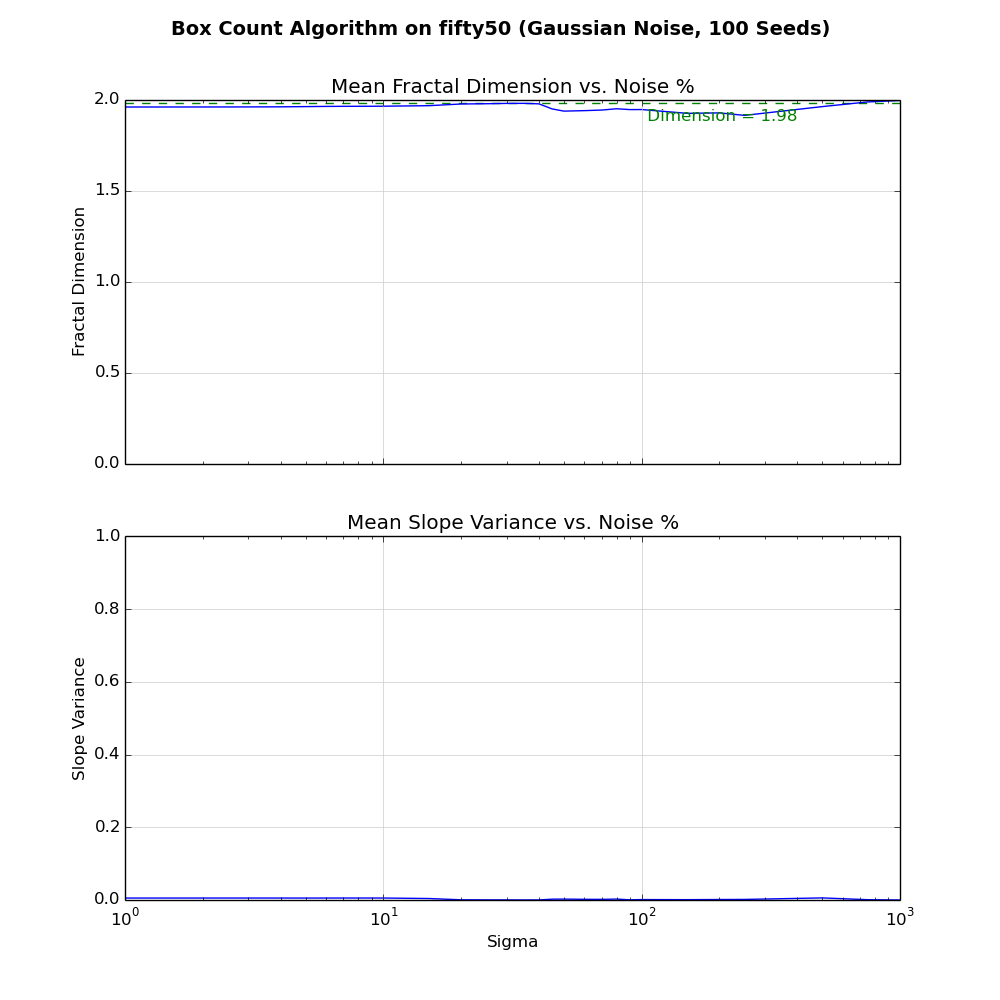
\includegraphics[width=\textwidth]{appendixD/Fig_Gaussian_DvSV_fifty50.png}}
  \caption[Fractal Dimension and Slope Variance vs. Gaussian noise for fifty50.png.]{Fractal Dimension and Slope Variance vs. Gaussian noise for fifty50.png.  Results shown are the average of 100 noise seeds.  Highlighted is initial no-noise dimensional estimate.}
  \label{fig:fifty50_gaussian_result}
\end{figure}

\begin{figure}[!b]
  \centering
  \frame{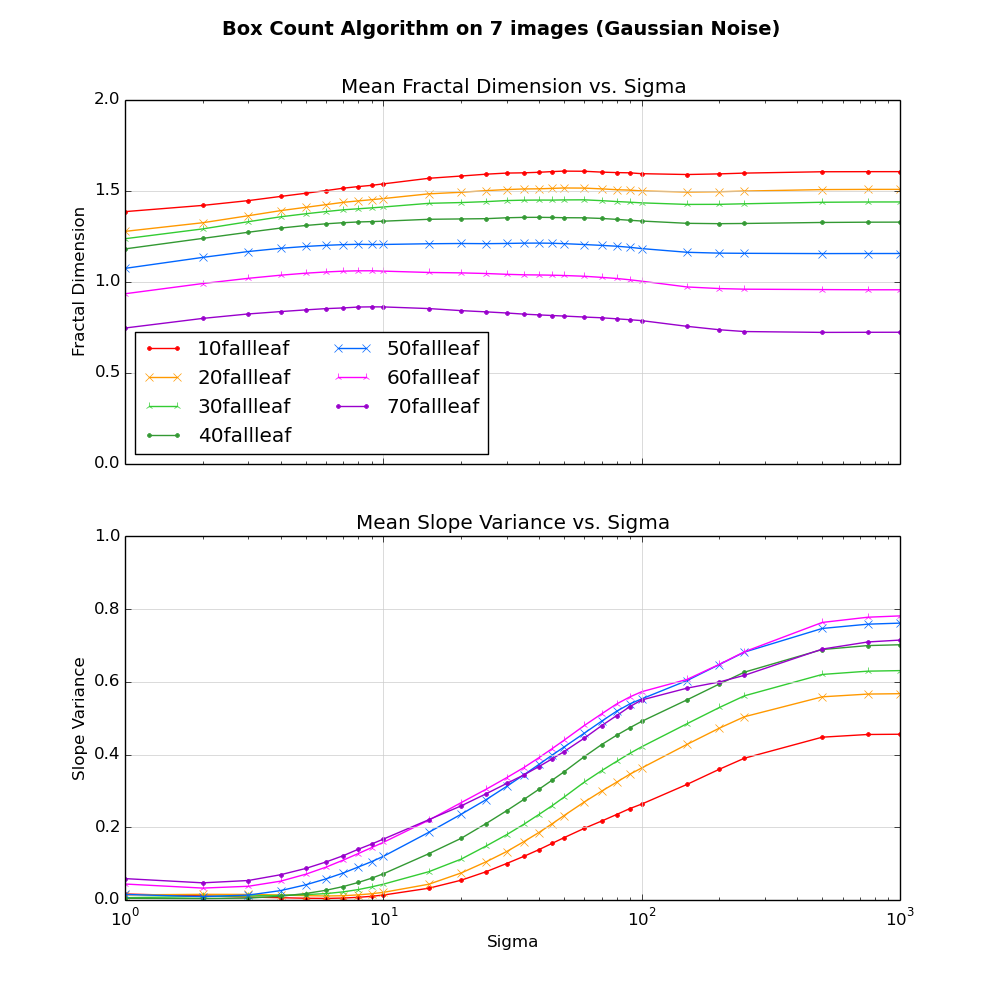
\includegraphics[width=\textwidth]{appendixD/Fig_DvsSV_Gaussian_Multiplot_70fallleaf.png}}
  \caption[Fractal Dimension and Slope Variance vs. Gaussian noise sigma value for leaf edge-detection filtered image set.]{Fractal Dimension and Slope Variance vs. Gaussian noise sigma value for leaf edge-detection filtered image set.  Results shown are the average of 100 noise seeds.}
  \label{fig:fallleaf_gaussian_multi_result}
\end{figure}

\begin{figure}[!b]
  \centering
  \frame{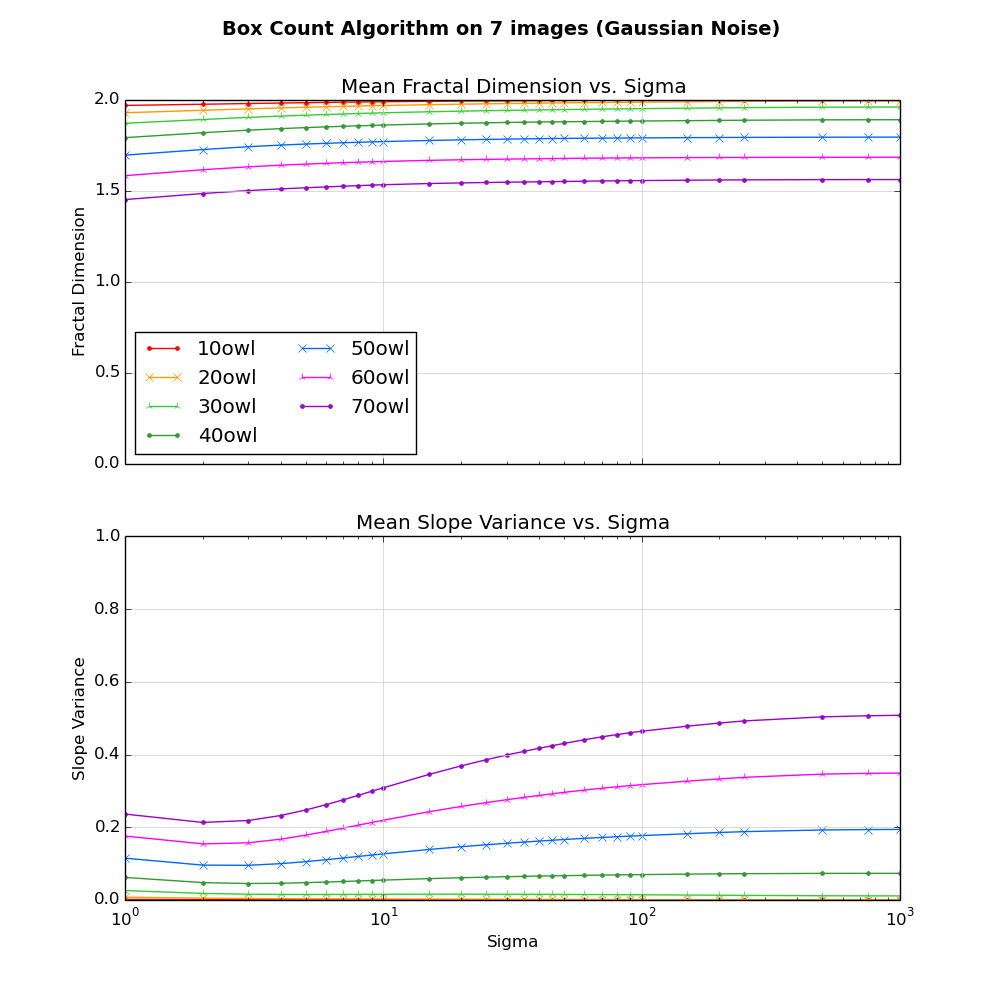
\includegraphics[width=\textwidth]{appendixD/Fig_DvsSV_Gaussian_Multiplot_70owl.png}}
  \caption[Fractal Dimension and Slope Variance vs. Gaussian noise sigma value for owl edge-detection filtered image set.]{Fractal Dimension and Slope Variance vs. Gaussian noise sigma value for owl edge-detection filtered image set.  Results shown are the average of 100 noise seeds.}
  \label{fig:owl-ed_gaussian_multi_result}
\end{figure}

%Fig50
\begin{figure}[!b]
  \centering
  \frame{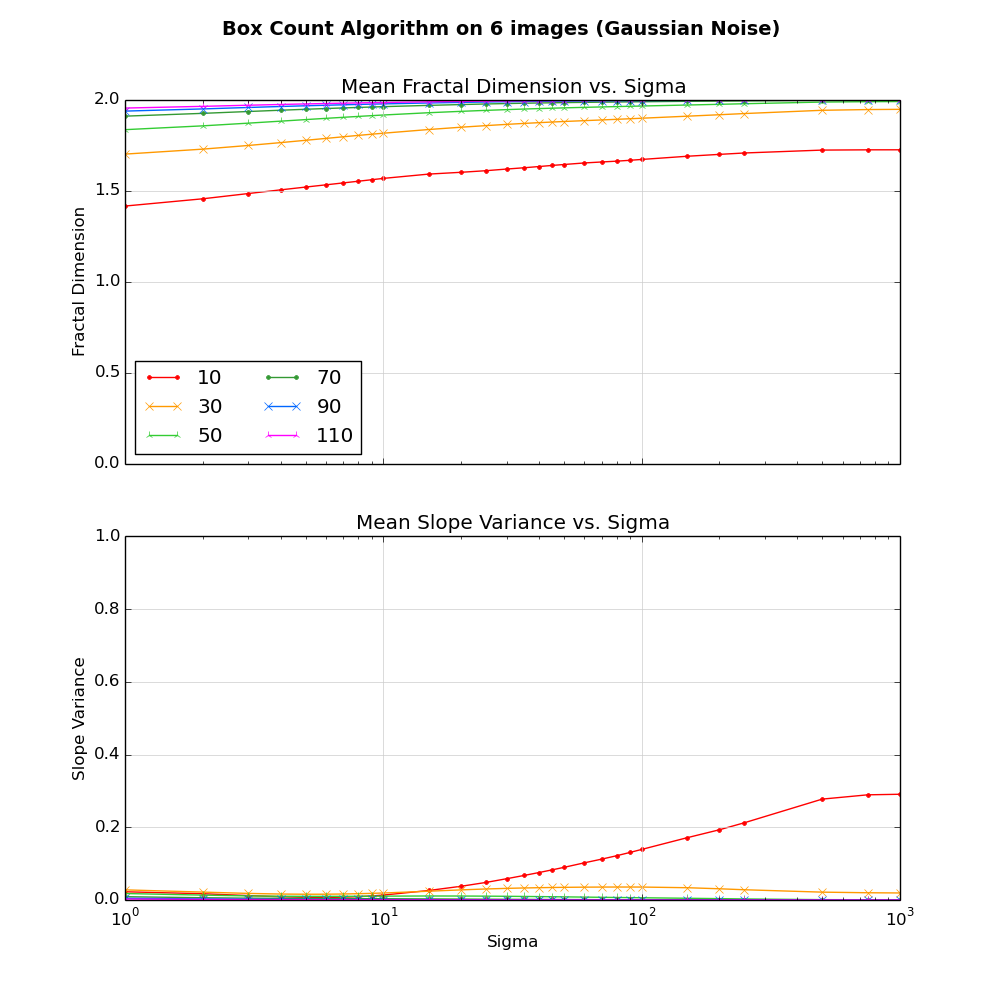
\includegraphics[width=\textwidth]{appendixD/Fig_DvsSV_Gaussian_Multiplot_110.png}}
  \caption[Fractal Dimension and Slope Variance vs. Gaussian noise sigma value for owl threshold filtered image set]{Fractal Dimension and Slope Variance vs. Gaussian noise sigma value for owl threshold filtered image set using threshold filters of 10, 30, 50, 70, 90, and 110.  Results shown are the average of 100 noise seeds.}
  \label{fig:owl-thresh_gaussian_multi_result}
\end{figure}


\clearpage



\end{document}